%************************************************************************
% ms2 Manual (Simon Stephan 2016)
% 
%
%************************************************************************


\documentclass[%
paper=A4,               % Papierformat
twoside=false,          % beidseitiger Druck (Koma-Script)
fontsize=11pt,          % Zeichensatzgroesse (Koma-Script)
headings=normal,        % Ueberschriftengroesse (alternativ big oder small, Koma-Script)
parskip=half+,          % Absatzkennzeichnung durch Zeilenabstand (Koma-Script)
numbers=noenddot,       % letzte Ziffer der Nummerierung ohne nachfolgenden Punkt (Koma-Script)
captions=tableheading,  % caption von Tabellen als Tabellenueberschrift formatieren (Koma-Script)
bibliography=totoc,     % Literaturverzeichnis in Inhaltsverzeichnis (Koma-Script)
listof=totoc,           % Tabellen- und Abbildungsverzeichnis in Inhaltsverzeichnis (Koma-Script)
index=totoc             % Index in Inhaltsverzeichnis (Koma-Script)
]
{scrbook}               % Dokumentklasse (alternativ scrartcl oder scrreprt, Koma-Script) 

% laedt die Bibliographie-Erweiterung biblatex
\usepackage[ %
backend=bibtex,         % Backend für biblatex [biber oder bibtex oder bibtex8]
style=authoryear, % authoryear oder numeric (-comp --> compress-Option)
bibstyle=authoryear,	% beeinflusst das Aussehen des Literaturverzeichnisses/ (reading oder authoryear etc.)
maxbibnames=10,        % max. Anzahl Namen im Literaturverzeichnis 
maxcitenames=1,        % max. Anzahl Namen bei authoryear Zitaten
backref=true,          % Literaturverzeichnis mit Verweis Zitat-Seiten 
%sorting=none,         % Verzeichnis nach Reihenfolge der Zitierung
dashed=false          % kein Strich im Verzeichnis bei Autor-Mehrfachnennung
%entryhead=true,		% für bibstyle "reading"
%entrykey=false			% für bibstyle "reading"
]
{biblatex}
% Anpassung Einzug und Absatzabstand an Dokumentlayout
\setlength{\bibhang}{0em} 
%\setlength{\bibitemsep}{\parskip}
\setlength{\bibitemsep}{0.5cm}
\setlength{\biblabelsep}{1cm}
% Einbindung der bib-Datei

\addbibresource{literatur_Manual.bib}		%fuegt .bib - Datei ein.



\newrobustcmd*{\parentexttrack}[1]{%
	\begingroup
	\blx@blxinit
	\blx@setsfcodes
	\blx@bibopenparen#1\blx@bibcloseparen
	\endgroup}

\AtEveryCite{%
	\let\parentext=\parentexttrack%
	\let\bibopenparen=\bibopenbracket%
	\let\bibcloseparen=\bibclosebracket}

% et al anstatt u.a. in einem Zitat
%\DefineBibliographyStrings{english}{ 
%	andothers = {{et\,al\adddot}},             
%} 



% Dokumenteinstellungen laden
% !TeX root = master_Manual.tex

%************************************************************************
% LaTeX Einstellungen (Simon Stephan 2016)
%
%
%************************************************************************


%************************************************************************
% Dokumenteinstellungen / Laden von Paketen
%
%************************************************************************

%\documentclass[%
%paper=A4,               % Papierformat
%twoside=false,          % beidseitiger Druck (Koma-Script)
%fontsize=11pt,          % Zeichensatzgroesse (Koma-Script)
%headings=normal,        % Ueberschriftengroesse (alternativ big oder small, Koma-Script)
%parskip=half+,          % Absatzkennzeichnung durch Zeilenabstand (Koma-Script)
%numbers=noenddot,       % letzte Ziffer der Nummerierung ohne nachfolgenden Punkt (Koma-Script)
%captions=tableheading,  % caption von Tabellen als Tabellenueberschrift formatieren (Koma-Script)
%bibliography=totoc,     % Literaturverzeichnis in Inhaltsverzeichnis (Koma-Script)
%listof=totoc,           % Tabellen- und Abbildungsverzeichnis in Inhaltsverzeichnis (Koma-Script)
%index=totoc             % Index in Inhaltsverzeichnis (Koma-Script)
%]
%{scrbook}               % Dokumentklasse (alternativ scrartcl oder scrreprt, Koma-Script) 

%Serifenlose Überschriften in KOMA-Script
\setkomafont{disposition}{\normalcolor\bfseries}

% Paket zur manuellen Randeinstellung
\usepackage{geometry}
\geometry{bindingoffset=10mm, left=15mm, right=15mm, top=20mm, bottom=25mm}

% Paket stellt die textblock-Umgebung zur Verfuegung, die frei auf der Seite
% platziert werden kann. Dabei koennen absolute Koordinaten (Papier) verwendet
% werden.
\usepackage[absolute]{textpos}


\usepackage{listings}
\usepackage{epsfig}
\usepackage{epstopdf}


% The bm pack­age de­fines a com­mand \bm which makes its ar­gu­ment bold
\usepackage{bm}


% Paket zur Gestaltung der Kolumnentitel
\usepackage{scrpage2}

% deutsche Trennungsregeln, deutsche Zusatzbefehle
\usepackage[english]{babel}

% Zeichenkodierung
\usepackage[utf8]{inputenc}

% deutsches Fontencoding, T1 Schriften
\usepackage[T1]{fontenc}

% Formatierung von Anführungszeichen --> \enquote Makro
% Option [german=guillemets] für französische Anführungszeichen
\usepackage{csquotes}

% Schriftfamilie ComputerModern Bright (serifenlos)
%\usepackage{cmbright}

% AMS-LaTeX Pakete fuer mathematischen Formelsatz. Die Option fleqn sorgt fuer
% linksbuendige Formeln, welche mit mathindent eingerueckt werden.
\usepackage[fleqn]{amsmath}
\usepackage{amssymb,amsthm}
\mathindent0.9cm

% stellt diverse Sonderzeichen zur Verfuegung z.B. \texteuro
\usepackage{textcomp}

% optischer Randausgleich (verschiedene Buchstaben, Satzzeichen, Bindestriche
% etc. werden leicht in den Seitenrand verschoben); automatische Skalierung von
% Buchstaben zur Verbesserung des Blocksatzes
\usepackage[tracking=true,spacing=true,kerning=true,final]{microtype}

% Silbentrennung wird auch bei linksbuendigem Text angewendet,
% z.B. im Index
\usepackage{ragged2e}

% das setspace package bietet die Moeglichkeit zur Aenderung des Durchschusses
% (Zeilenabstand im Blocksatz)
\usepackage{setspace}

% zusaetzliche Hinweise zur Seite auf der sich ein Verweis befindet
% z.B. mit dem Befehl \vref{label}
\usepackage[english]{varioref}

%% laedt die Bibliographie-Erweiterung biblatex
%\usepackage[ %
%backend=biber,         % Backend für biblatex [biber oder bibtex]
%style=authoryear-comp, % authoryear oder numeric (-comp --> compress-Option)
%maxbibnames=10,        % max. Anzahl Namen im Literaturverzeichnis 
%maxcitenames=1,        % max. Anzahl Namen bei authoryear Zitaten
%backref=true,          % Literaturverzeichnis mit Verweis Zitat-Seiten 
%%sorting=none,         % Verzeichnis nach Reihenfolge der Zitierung
%%dashed=false          % kein Strich im Verzeichnis bei Autor-Mehrfachnennung 
%]
%{biblatex}
%% Anpassung Einzug und Absatzabstand an Dokumentlayout
%\setlength{\bibhang}{0em} 
%\setlength{\bibitemsep}{\parskip}
%% Einbindung der bib-Datei
%\addbibresource{literatur.bib}

% Grafikunterstuetzung fuer LaTeX (Einfuegen von Bildern)
\usepackage{graphicx}

% Anordnung mehrerer Grafiken
\usepackage{subfig}

% Paket zum Drehen von Text, Tabellen, Grafiken etc.; das Paket stellt dafür
% die landscape-Umgebung zur Verfuegung
\usepackage{lscape}

% float-Objekte werden nur innerhalb der aktuellen section verschoben, ohne
% dieses Paket koennen floats auch in die naechste section uebernommen werden
\usepackage[section]{placeins}

% laedt das Grafikpaket tikz sowie einige Bibliotheken dazu
\usepackage{tikz}
\usetikzlibrary{arrows,shapes}


% Paket zum Setzen von Einheiten und zur Formatierung von Zahlen
% Einheiten werden immer "gerade" gesetzt. Zahlenformate, Trennzeichen etc.
% werden anhand der Spracheinstellungen (babel) ausgewaehlt (Manuelle
% Vorgaben sind ebenfalls moeglich --> siehe Paketdoku siunitx). 
% Befehle: \SI{Zahl}{Einheit}, \num{Zahl}
\usepackage[ngerman]{translator}
\usepackage[locale=DE, separate-uncertainty=true]{siunitx}

% Paket zum Erstellen neuer Spaltentypen
% --> Übergabe des Zelleninhaltes an Makros
\usepackage{collcell}

% mhchem Paket zum Setzen chemischer Formeln mit dem \ce Makro. Bei
% Verwendung im Text (ohne Mathe-Umgebung) wird die Schriftart automatisch
% an den umgebenden Text angepasst (Überschriften etc.).
\usepackage[version=3,arrows=pgf]{mhchem}
% Umbiegen des \ce Makros --> Für hyperref-Links wird der Quellcode der
% Formel als Linktext verwendet. Bei Nutzung des Makros in Überschriften 
% erscheinen sonst kryptische Linknamen, da im PDF dafür Sonderzeichen
% nicht erlaubt sind.
\let\oldce\ce
\renewcommand{\ce}[1]{\texorpdfstring{\oldce{#1}}{#1}}
% Neuer Spaltentyp für Tabellen mit \ce Makro
\newcolumntype{C}{>{\collectcell\ce}{l}<{\endcollectcell}}

% fuegt longtable-Umgebung ein (Tabellen mit moeglichem Seitenumbruch)
\usepackage{longtable}

% tabularx-Umgebung ermoeglicht Tabellen mit fester Breitenvorgabe,
% zusaetzlicher Spaltentyp X fuellt Tabelle auf Breitenvorgabe auf
\usepackage{tabularx}

% erweiterte Tabellenbefehle (zur Erstellung wirklich schoener Tabellen
% fuer den Buchdruck)
\usepackage{booktabs}

% erweiterte Moeglichkeiten zur Schriftformatierung in Tabellenspalten
\usepackage{array}

% Paket zum Zusammenfuegen von Tabellenzeilen
\usepackage{multirow}

% Paket zur Indexerstellung,  Indexeintraege mit \index{Name des Eintrages}
\usepackage{makeidx}
\makeindex

% erstellt Anweisungen, die nur fuer pdftex gelten
\usepackage{ifpdf}

% implementiert if Schleifen
\usepackage{ifthen}

% Paket zur automatischen Linkerstellung fuer Inhaltsverzeichnis, Literaturverweise etc.
% [plainpages=false] setzt getrennte Links fuer gleiche Seitenzahlen (z.B. fuer i und 1)
% [pdfpagelabels] geaendertes Anzeigeformat der Seitennummern im AcrobatReader (roemische
% Seitennummern werden angezeigt)
\usepackage[plainpages=false, pdfpagelabels]{hyperref}

% setzt Strafpunkte fuer Schusterjungen und Hurenkinder hoch 
\clubpenalty=10000
\widowpenalty=10000
\displaywidowpenalty=10000


%************************************************************************
% Anpassungen Kolumnentitel und Schriftarten
%
%************************************************************************

% Anpassung der Kolumnentitel, Seitennummerierung oben, Schriftgroessen
\clearscrheadfoot
\ohead{\headmark}
\ofoot[\pagemark]{\pagemark}
\pagestyle{scrheadings}
\addtokomafont{pageheadfoot}{\footnotesize}

% kleinere Schriftgroesse fuer Bildunterschriften/Tabellenueberschriften
\addtokomafont{caption}{\footnotesize}

% Anpassungen fuer das cmbright-package
% demibold (anstatt bold) als Fettschrift verwenden
%\renewcommand{\bfseries}{\fontseries{sb}\selectfont}
%% Befehl \textbx fuer Fette zur Verfuegung stellen 
%\newcommand{\textbx}[1]{{\fontseries{b}\selectfont#1}}
%\newcommand{\bxseries}{\fontseries{b}\selectfont}
% Ueberschriften in LatinModernSans-demicondensed
\newcommand{\headFont}{\fontfamily{lmss}\fontseries{sbc}\selectfont}
\addtokomafont{disposition}{\headFont}
% \mathsf fuer cmbright richtig definieren
% (sonst wird bei \mathsf CM-SansSerif verwendet)
\renewcommand{\mathsf}[1]{\mathrm{#1}}

\def\dcoeff{{\ooalign{\raisebox{.5mm}{\text{--}}\hspace{-1.9mm}}\hbox{\textit{\textbf{D}}}}}


%************************************************************************
% Definition Styles und Farbschemen
%
%************************************************************************

\makeatletter

% Voreinstellungen
\def\@docstyle{report}
\def\@color{white}

% Makro zur Auswahl von Style und Farbschema
\newcommand{\setlayout}[2]{%
  \def\@docstyle{#1}
  \def\@color{#2}
  \@setlayout
}


% Makro zur Umsetzung von Style und Farbschema
\newcommand{\@setlayout}{%
  % Farbschema weiss
  \ifthenelse{\equal{\@color}{white}}{% 
  }
}


%************************************************************************
% Titelseite
%
%************************************************************************

% Variablen fuer Benutzereinstellungen
\def\@faculty{}
\def\@chair{}
\def\@subTitle{}
\def\@titleFoot{}

\newcommand{\faculty}[1]{\def\@faculty{#1}}
\newcommand{\chair}[1]{\def\@chair{, #1}}
\newcommand{\subTitle}[1]{\def\@subTitle{#1}}
\newcommand{\titleFoot}[1]{\def\@titleFoot{#1}}

\renewcommand{\maketitle}{%
  \begin{titlepage}
    \null%
    \begin{textblock*}{297mm}(0mm,0mm)%
    {\setlength{\unitlength}{1mm}%
    \noindent%
    \begin{picture}(0,0)%     

      \ifthenelse{\equal{\@color}{white}}{%  

        \def\@headfontcolor{\color{black}}
        \def\@textfontcolor{\color{black}}
        \def\@logofile{grafiken/logos/Logo_LTD_Text}
      }

      
      % Minipage als Bereich fuer den Seiteninhalt     
      \put(30,-44){\@textfontcolor
        \begin{minipage}[t][140mm][l]{160mm}

            \vfill
            \vfill
            \vfill
            \vskip 2em
            \begin{center}
              {\headFont\Huge\@title}
              \vskip 1em
              \textbf{\Large\@subtitle}
            
            \vskip 1.5em
              \Large\@subTitle
            
            \vskip 3em
            {\large\@date}      
            \vfill
            \phantom{x}
            \end{center}

       \end{minipage} 
      }

      % Infoblock Fusszeile (in fester Schriftgroesse)
      \put(30,-280){\@headfontcolor\fontsize{8pt}{10pt}\selectfont
        \begin{minipage}[t][21mm][l]{160mm}
          {\setlength{\tabcolsep}{1.5em} %groesserer Spaltenabstand
          \@titleFoot
          }
        \end{minipage}
      } 
    \end{picture}
  }
  \end{textblock*}
\end{titlepage}
}


%************************************************************************
% pdf Dokumenteninformationen (Datenübernahme aus Titelangaben)
%
%************************************************************************

\newcommand{\makepdfinfos}{%
  \hypersetup{  
    pdfauthor = {\@author},
    pdftitle = {\@title},
    pdfsubject = {\@subTitle},   
    pdfkeywords = {},
    bookmarksnumbered = {true}, % Lesezeichen im pdf mit Nummerierung
    pdfpagemode = {UseOutlines}, % UseOutlines, UseThumbs, None
    pdfstartview = {FitH}, % FitH, FitV oder XYZ null null 0.9
    pdffitwindow = {true}, % Fenstergröße anpassen
  }
}



\makeatother

%%% Local Variables: 
%%% mode: latex
%%% TeX-master: "master"
%%% coding: utf-8
%%% End:



% Layout des Dokumentes festlegen
% Style [report/thesis] und Farbschema [white/blue/bluewhite]  
\setlayout{report}{white}


%************************************************************************
% Dokumenteninformationen 
%
%************************************************************************

\faculty{Fakultät Maschinenbau und Verfahrenstechnik}
\chair{Professur für Thermodynamik -- Technische Universität Kaiserslautern}


\title{Manual \textit{ms}2}
\subtitle{A Molecular Simulation Tool for Thermodynamic Properties}
\date{Kaiserslautern, März 2016}




% Dokumentinfos ins pdf übernehmen
\makepdfinfos


\begin{document}


%************************************************************************
% Vorspann
%
%************************************************************************

% Zeilenabstand einzeilig
\singlespacing
\frontmatter

% Titelseite erzeugen
\maketitle

% Einfügen des Inhaltsverzeichnisses
\tableofcontents

%************************************************************************
% Hauptteil
%
%************************************************************************

\singlespacing
\mainmatter

% Einfügen der einzelnen Kapitel



\chapter{Introduction}
\label{sec:Introduction}



\section{Program summary}
\label{sec:Program Summary}
% Simon


\textit{ms}2 has been successfully used in the Industrial Fluid Properties Simulation Challenge \parencite{fluidproperties}. It is a molecular simulation program that aims at the calculation of thermodynamic properties that are needed for applications in the chemical industry, without requiring expert knowledge by the user. It was developed for rigid molecular models with a focus on condensed phases, covering mixtures containing an arbitrary number of small molecular species.

The simulation program \textit{ms}2 is optimized for a fast execution on a broad range of computer architectures, spanning from single processor PCs over PC clusters and vector computers to high end parallel machines. It is a standalone Fortran90 code that does not require any libraries and does not have any other software prerequisites. \textit{ms}2 is provided as a source code and it only needs to be compiled. The structure of \textit{ms}2 is modular and object-oriented, except at the very core of energy and force calculations, where some structural compromises were made to achieve a better performance.

\textit{ms}2 is aimed at homogeneous bulk systems in equilibrium and contains a molecular dynamics (MD) and Monte Carlo (MC) sampling. For vapour-liquid equilibrium (VLE) calculations, the coexisting phases are simulated independently and sequentially. Thus, it is usually sufficient to sample molecular systems containing on the order of $10^{3}$  molecules to obtain statistically reliable results \parencite{lyubartsev}. Applying standard cut-off radii, the intermolecular interactions are evaluated roughly up to the maximal distance, which is given by the edge length of the cubic simulation volume. Therefore, spatial decomposition schemes for parallelization are not rewarding. Instead, Plimpton's method \parencite{plimpton} was implemented for parallel execution of MD, which scales reasonably well up to 16 or 32 processors, depending on the particular architecture. For MC, an optimal parallelization scheme was introduced, taking advantage of the stochastic nature of such simulations. The computing resources are splitted into single runs each on one node, sampling the phase space independently. Both parallelization methods allow for short response times\footnote{Under "response time" we understand the real time difference between submission and termination of a simulation run.}. A typical molecular simulation of a VLE state point takes roughly six hours on a current workstation. The main expenses for determining thermodynamic data in silico are installation and maintenance of computing equipment and/or computing time, which is presently below US$\$$ 0.35/CPU-hour \parencite{economist}.

The simulation program \textit{ms}2 presented here was developed in a long-standing and ongoing cooperation of engineers and computer scientists. With the current version 3.0 of \textit{ms}2, it is intended to facilitate the transfer of a state of the art and user-friendly molecular modeling and simulation package to academic institutions and the chemical industry. The release package consists of the simulation program \textit{ms}2 itself and auxiliary feature tools for setup and analysis of simulation runs, including a simple 3D visualization tool to monitor the molecular trajectories. Furthermore, accurate force field models for more than 100 small molecules are provided.

%In section 2 of this manual, the installation of \textit{ms}2 is described on different platforms. Section 3 introduces the implemented molecular simulation techniques. In sections 4 and 5, \textit{ms}2 and the implemented thermodynamic properties are outlined. Section 6 gives details on executing \textit{ms}2, while section 7 provides some examples to demonstrate the use of the simulation program. Section 8 presents runtime tests and section 9 describes the auxiliary feature tools. Section 10 of this manual comments on adaptations of the software. In section 11 the error messages are addressed.






\section{Citation information \& license}
\label{sec:Citation information}
% Simon

\textit{ms}2 is a noncommercial software, which was published in Computer Physics Communications. The most current manuscript as the preceding ones along with their Supplementary Materials can be downloaded from the \textit{ms}2 home page (\href{http://www.ms-2.de}{\textit{http://www.ms-2.de}}). It is free of charge for scientific research and can be obtained after registration. Users need to acknowledge the use of \textit{ms}2 by citing the following publication:
\begin{itemize}
	\item[ ] S. Deublein, B. Eckl, J. Stoll, S. Lishchuk, G. Guevara-Carrion, C.W. Glass, T. Merker, M. Bernreuther, H. Hasse, J. Vrabec
	\item[ ] Computer Physics Communication \textbf{182} (2011) 2350
	\item[ ] doi:10.1016/j.cpc.2011.04.026
\end{itemize}
%The paper along with its Supplementary Material can be downloaded from the \textit{ms}2 home page. 
%Users need an user account that can also be requested on the above mentioned website. Any use of the software shall only be for purposes of research and academic teaching. There is no license or registration fee. Use in connection with a business purpose is not permitted. Transferring the Software to third parties is not allowed. The Laboratory of Engineering Thermodynamics (LTD), as the supplier of \textit{ms}2, provides the Software without any guarantee obligation or any warranty as to its features and gives no guarantee that the Software is free from faults.

%In order to register as an \textit{ms}2 user, it is necessary to enter into a contract with the University of Kaiserslautern and the LTD. In the context of this contract the user shall be entitled to adapt, modify and copy the software \textit{ms}2. The user is encouraged but not obliged to inform LTD about contributions and results, in particular adaptations of the software and new programs, arising in connection with the software. 


The \textit{NonCommercial 3.0} (CC by-NC 3.0) licence applies for \textit{ms}2. The full licence is available under (\href{https://creativecommons.org/licenses/by-nc/3.0/legalcode}{creative commons}. You may not use the material for commercial purposes. You must give appropriate credit, provide a link to the license, and indicate if changes were made. You may do so in any reasonable manner, but not in any way that suggests the licensor endorses you or your use. You are free to share a copy and redistribute the material in any medium or format and adapt, transform, and build upon the material. 





\section{Support, development \& maintenance}
\label{sec:Support, Development maintenance}
% Simon

Supply the version and compiling details with a support request.

The newest version of the \textit{ms}2 molecular simulation package is available at the \textit{ms}2 homepage:
\begin{itemize}
	\item[ ] \href{http://www.ms-2.de}{\textit{http://www.ms-2.de} }
\end{itemize}
The source code of \textit{ms}2 can be downloaded there as a tarball. 

The following email address is the general contact point:
\begin{itemize}
	\item[ ] \textit{contact@ms-2.de}
\end{itemize}
\textit{ms}2 users are encouraged to report bugs to the aforementioned email address.






\chapter{Installation}
\label{sec:Installation}



\section{Downloading the source code}
\label{sec:Downloading the source Code}
% Simon
The \textit{ms}2 distribution is available on the webpage: \href{http://www.ms-2.de/download}{http://www.ms-2.de/download}. Users must either be a natural person or an academic institution represented by a natural person. The \textit{ms}2 distribution consists of four major parts: the source code, java tools for pre- and postprocessing, force field models from the \href{http://thermovm.mv.uni-kl.de/moleculeDB/}{\textit{Molecular Models of the Boltzmann-Zuse Society}} database as input files for \textit{ms}2 and some example input files for the calculation of different properties. The installation and use of the \textit{ms}2 program is explained in detail in section \ref{sec:Runningms2}, \ref{sec:Keywords} to \ref{sec:Methods}. The application of the java tools is shown in section \ref{sec:Tools}. A detailed list of the force fields that comes with the \textit{ms}2 distribution is in section \ref{sec:Potential Models in the ms2-distribution}. 
%The examples are explained in section xx of this manual. 



% Verisionen -> Zugang zu älteren Versionen?!
% 
% Zugang zum Code: Kommerziell und akademische Zwecke?!
% user account anlagen..





\section{Building \textit{ms}2}
\label{sec:Compiling ms2}
\textit{ms}2 is tested on Linux and Windows platforms, a short explanation how to install the \textit{ms}2 on these two systems is given in the following.

% Hier noch ein paar Allgemeine Sätze/ wie toll es auf Großrechnern läuft 

\subsection{Building \textit{ms}2 on Linux platforms}

% kann das makefile.mult aus dem trunk raus?! Oder sollte es hier zusätzlich erwähnt werden?!


The compilation can be carried out using the provided ``Makefile'' found in the ``src'' directory (e.g.\ with \href{http://www.gnu.org/software/make/}{GNU make}) and the compiler-related \texttt{*.mk}-files in the \texttt{makefiles}-subdirectory. The ``Makefile'' and the ``\texttt{*.mk}''-file should be adopted to the local system requirements as described below. Alternatively (or additionally) variables can be set through the make command line options as compiler flags. An overview of all options can be found in table \ref{tab:makefiledef}.\\
When compiling \textit{ms}2, a variety of settings can be specified according to the users needs and optimise the performance. The following strings are recognized in the makefile: \texttt{TARGET}, \texttt{RELEASE}, \texttt{MPI}, \texttt{OMP}, \texttt{TRANS}, \texttt{HBOND}, \texttt{OSMOP}, \texttt{SP} and \texttt{PROG}. After settings these variable according to the users hardware and computational need, typing \texttt{make} in the command line from the ``src'' directory compiles \textit{ms}2 and creates and executable in the current directory.

%There's also an obsolete ``Makefile.mult'' containing compiler options that have been used in the past (for systems, which might be already out of service today).

\textbf{Settings in the \texttt{Makefile}}\\
First of all a compiler has to be chosen. Through the definition of the \texttt{COMPILER} variable, the corresponding file with suffix ``.mk'' in the ``makefiles'' subdirectory will be included during the execution of \texttt{make}. These files contain specific settings for compilers and/or systems that \textit{ms}2 is suitable for.\\
\begin{itemize}
	\item Version:\\
	\texttt{TARGET~=~RELEASE} or \texttt{DEBUG}\\
	The \texttt{DEBUG} version is manly used by developers. Default is \texttt{RELEASE}.
	\item FORTRAN Compiler:\\
	\texttt{COMPILER~=~INTEL}, \texttt{GNU} or \texttt{PGI}\\
	The entry \texttt{GNU} found in the given Makefile corresponds to ``makefiles/GNU.mk'', which contains settings for the widely used \href{http://www.gnu.org/software/gcc/}{GNU compiler}. There are other predefined settings available, like ``INTEL'' for the \href{https://software.intel.com/en-us/intel-compilers}{INTEL compiler}. The default value is \texttt{GNU}, since that compiler is freeware. 
%	(@Martin: hier auch die Cray und Ace compiler aufnehmen?)   Auch etwas zu pgi schreiben?
	\item Parallelisation protocol:\\
	\texttt{MPI~=~1} or \texttt{0} or \\
	\texttt{OMP~=~1} or \texttt{0}\\
	These parameters have to be set to invoke the implemented parallelisation schemes. 
\end{itemize}
The make command produces one executable file of \textit{ms}2. To optimise the execution speed of the program for each application, the user should set the Feature Compiler Flags \texttt{TRANS}, \texttt{HBOND}, \texttt{OSMOP} and \texttt{SP} according the Simulation dependencies -- especially if the user wants to run large numbers of simulations with one executable. We suggest only to set a \texttt{Compiler Variable = 1} if you want to use this certain feature, otherwise they will slow down your simulation speed.
\begin{itemize}
	\item Transport properties:\\
	\texttt{TRANS~=~1} or \texttt{0}\\
	To produce an executable that samples transport properties (like diffusion and conductivity)  \texttt{TRANS~=~1} has to be set. A value of \texttt{0} means that the routines for the calculation of transport properties are not compiled. The default value is \texttt{0}, since the program execution for the sampling of the default properties is faster in that case.
	\item Hydrogen-bonding evaluation:\\
	\texttt{HBOND~=~1} or \texttt{0}\\
	If you want to have a look at the H-Bonds in your system, turn this on (set variable \texttt{1}). % See chapter \ref{sec:H-Bonding} for more information. 
	It enables you to specify a geometric criterion for H-bonds in your input files. \textit{ms}2 plots then the pursuant H-bonding statistics. A Value of \texttt{0} means, that the routines for the calculation of H-bonds are not to be compiled. The default value is \texttt{0}, since the program execution for the sampling of the default properties is faster in that case.
	\item Osmotic pressure:\\
	\texttt{OSMPO~=~2}, \texttt{1} or \texttt{0}\\
	This flag enables the osmotic pressure method% described in section \ref{sec:OsmoticPressure}
	. The value \texttt{2} enables the pressure profile along the density profile and osmotic pressure results. %was macht der Value 1?!?!?
	 A Value of \texttt{0} means, that the routines for use of the osmotic pressure method are not to be compiled. The default value is \texttt{0}.
	 \item Single precision:\\
	 \texttt{SP~=~1} or \texttt{0}\\
	 To speed up your simulation you can choose single precision (set value \texttt{1}) instead of the default double precision  (set value \texttt{0}). Users are advised to use \texttt{SP~=~1} with care.
	 \item Name of the executable file:\\
	 \texttt{PROG~=~String}\\
	 The user can set the value to adapt the name of the executable file that is produced by the make command. According to the values of \texttt{TRANS}, \texttt{HBOND}, \texttt{OSMOP}, \texttt{SP}, \texttt{COMPILER} and \texttt{TARGET} the executable will have an addition in its name respectively.
\end{itemize}

% Beispiel Tabelle machen?!?!

% ARCH = 1, 2 or 3
%@Martin: Da bin ich überfragt, was die Unterschiede angeht und raten auf Grund des source codes ist auch blöd.
% FORTRAN = 90 (@Martin: gibt es da andere möglichkeiten? Wird im source code, wenn dann nur als 90 definiert, aber nie verwendet.)
%Compiler flags

\renewcommand{\arraystretch}{1.2}
\begin{table}[h!]
	\centering
	\begin{tabular}{llll}
		\toprule
		Variable & Description & Values & Description \\
		\midrule
		&                           &  &  \\
		
		\multicolumn{4}{l}{{Compiler settings:}}\\
		\midrule
		\texttt{COMPILER} & Compiler presets          & \texttt{GNU}   & \href{http://www.gnu.org/software/gcc/}{GNU compiler} \\
		&                           & \texttt{INTEL} & \href{https://software.intel.com/en-us/intel-compilers}{INTEL compiler} \\
		&                           & \texttt{PGI} & PGI compiler \\
		&                           & {\tiny see makefiles subdirectory} \\
		
		\texttt{TARGET}   & see above                 & \texttt{RELEASE} & for production simulations \\
		&                           & \texttt{DEBUG} & for code developing   \\
		
		\multicolumn{4}{l}{{Parallelization setting:}}\\
		\midrule
		\texttt{MPI}      & \href{http://mpi-forum.org/}{MPI} & \texttt{0} & off \\
		&                                   & \texttt{1} & on \\
		&                           &  &  \\
		
		\texttt{OMP}      & \href{http://openmp.org/}{OpenMP} & \texttt{0} & off \\
		&                                   & \texttt{1} & on \\
		
		\multicolumn{4}{l}{{Features to be accessible:}}\\
		\midrule
		\texttt{SP}       & Single Precision          & \texttt{0} & off \\
		&                           & \texttt{1} & on \\
		&                           &  &  \\
		
		\texttt{TRANS}    &        Transport          & \texttt{0} & off \\
		&                           & \texttt{1} & on \\
		&                           &  &  \\
		
		\texttt{OSMOP}    &         Osmotic pressure  & \texttt{0} & off \\
		&                           & \texttt{1} & on \\
		&                           &  &  \\
		
		\texttt{HBOND}    &     H-Bonding statistics  & \texttt{0} & on \\
		&                           & \texttt{1} & on \\
		&                           &  &  \\
		
		\texttt{PROG}    &     Name of executable  & String & can be set by user \\
		\bottomrule
	\end{tabular}
	\caption{Makefile definitions}
	\label{tab:makefiledef}
\end{table}
% was ist mit PGI in Tabelle?!
\renewcommand{\arraystretch}{1}

\pagebreak


\textbf{Compiler-related \texttt{*.mk} files}\\
For each supported compiler, the subdirectory \texttt{makefiles} in \texttt{src} contains one \texttt{*.mk} file, e\,g. \texttt{INTEL.mk}. The first three lines define the used FORTRAN90 comilers. In rare system depending cases, the optimisation degree (the integer after the -O for the \texttt{F90FLAGS\_RELEASE} has to be decreased to 2 or 1). It is suggested to use the slightly faster \texttt{mpiifort}-Compiler instead of the \texttt{mpiF90} in case you are using the \texttt{INTEL.mk}.

\textbf{make command line options}\\
Instead of changing the Makefile, the definitions can also be set directly in the command line, that will overwrite the settings in the makefile. For example:\\

%\begin{lstlisting}
\texttt{make TARGET=RELEASE COMPILER=GNU}


%\end{lstlisting}
%These settings will overwrite the ones in the Makefile.

\paragraph{Compiler Flags}


Depending on compiler and preprocessor variables set in the makefile, the following compiler flags are used in the compilation/build process:
\begin{itemize}
	\item[] OMPFlags: -mp/openmp/fopenmp
	\item[] CPPFlags: -DARCH=2 –DFORTRAN=90 (replaces compiler flags for ARCH and FORTRAN)
	\item[] Releaseflags: -O3 -vec/qopt-report=3/5
	\item[] Debugflags: -O0 -vec/qopt-report=0 -g
	\item[] GNU: -ffree-line-length-none -mtune=generic
	\item[] INTEL: -fpp –r8
	\item[] PGI: -C
\end{itemize}
If the user is unsure what compiler flags to set, it is suggested to leave the make file blank.
% gab es nicht einen Flag um den Namen der executable zu definieren?!



	

% Hier ein Beispiel mit Erläuterung einbauen!!!!



\subsection{Building on Windows}
\textit{ms}2 can also be executed on windows systems. The source code has to be downloaded and compiled in a similar way as for Linux platforms. It is suggested to use a Linux-like shell, for example \href{https://www.cygwin.com}{\textit{cygwin}}. It provides a terminal window that runs a handsome Linux shell and comes with the \textit{GNU gfortran} compiler\footnote{during the installation of cygwin, all the FORTRAN depending packages have to be tagged.}. This is very useful, since \textit{ms}2 is a command line-based program whose utilisation is in our experience best in combination with the standard Linux commands, such as \texttt{sed}, \texttt{awk}, \texttt{grep}, \texttt{find} etc.. Additionally, the preparation of input files and analysis of the output files of \textit{ms}2 can be done by shell scripts. The installation of \textit{ms}2 in \textit{cygwin} follows the installation instructions on Linux platforms discussed above. Of course, \textit{ms}2 can also be compiled using standard windows tools.






\chapter{Running \textit{ms}2}
\label{sec:Runningms2}
% Simon

\textit{ms}2 was designed to be an easily applicable simulation program. Therefore, the input files are restricted to one file for the definition of simulation scenario and one file for each of the molecular species that are used in the simulation. The output files contain structured information on the simulation. All calculated thermodynamic properties are summarized in one output file, which is straightforwardly readable and self-explaining. For a more detailed evaluation of the simulation, the instantaneous and running averages of the most important thermodynamic properties are written to other files. In total, the current status of the simulation and many more details are written to six files and can be accessed during execution. The structure of the input files as well as the output files is shown in Figure~\ref{fig:File-structure}.
\begin{figure}[h]
	\centering
	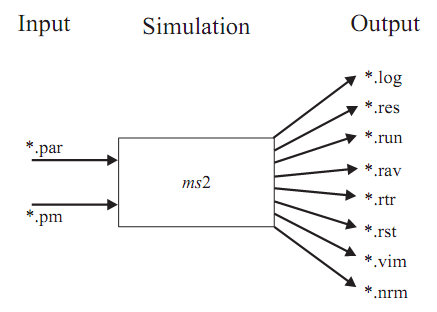
\includegraphics[width=0.55\columnwidth]{fig_structure.png}
	\caption{File structure needed and generated by \textit{ms}2.}
	\label{fig:File-structure}
\end{figure}




%
%
%\section{Running \textit{ms}2 on Windows or Linux}
%\label{sec:Running ms2 on Windows or Linux}
%% Simon
%
%\textbf{Restart a Simulation with \texttt{*.rst} file}
%


%
%\section{Running \textit{ms}2 in serial or parallel mode}
%\label{sec:Running ms2 in serial or parallel mode}
%% Simon


%
%
%\section{Flowchart}
%\label{sec:Flowchart}
%%Simon
%



\section{Input structure}
\label{sec:Input structure}
%Simon

\textit{ms}2 expects two input files: the \texttt{$^{*}$\hspace{-3pt}.par} and the \texttt{$^{*}$\hspace{-3pt}.pm} file. The \texttt{$^{*}$\hspace{-3pt}.par} file specifies the simulation \underline{par}ameters and the \texttt{.pm} file the molecular \underline{p}otential \underline{m}odel. The \texttt{$^{*}$\hspace{-3pt}.par} file is the main file steering the actual simulation. It contains all input variables for the simulation process, such as simulation type, ensemble, number of equilibration and production steps, time step length etc. Also the potential models need to be declared here. Each \texttt{$^{*}$\hspace{-3pt}.pm} file specifies exactly one chemical substance. To calculate mixtures, several \texttt{$^{*}$\hspace{-3pt}.pm} files have to be specified in the \texttt{$^{*}$\hspace{-3pt}.par} file.

Each line in both input file types sets one parameter, is empty or contains a comment. The comment symbol $\#$ and everything after it up to the end of the line is ignored by \textit{ms}2 in the same way as empty lines are. It is suggested to use only blanks instead of tabs, since the latter may cause trouble using input files generated on other platforms. 

A line setting a parameter in either \texttt{$^{*}$\hspace{-3pt}.par} or \texttt{$^{*}$\hspace{-3pt}.pm} file always consists of a keyword \texttt{XXX}, the \texttt{=} symbol and the parameter value YYY, e.\,g. \\
\texttt{NVTSteps  =  100000}\\
Leading spaces, trailing spaces and spaces surrounding = symbol are ignored. Parameter values can be strings in some case or numeric values. Parameter names and values that \textit{ms}2 expects for the parameter file and potential model files are described in sections \ref{sec:Keywords}. All parameters must be present in the input files in the certain order. The program reads the input file sequentially. % stimmt das noch? -> Martin B. fragen
Unidentified parameters are ignored. Missing or misplaced parameters lead to the termination of the program with the corresponding error message.


\subsection{Parameter file}
\label{sec:par - file}
% Simon

Below is an exemplary  \texttt{$^{*}$\hspace{-3pt}.par} file for a MD simulation of pure oxygen in the $NVT$ ensemble.  \texttt{$^{*}$\hspace{-3pt}.par} files are organised in three sections: the first section sets the general simulation parameters, such as timestep, MD or MC, unit systems etc. (lines 3 to 20 in the oxygen example), the second section sets the thermodynamic quantities to define the ensemble, such as temperature, density, number of components etc. (lines 21 to 26). The third section contains the potential models that shall be simulated and indicate their mole fraction (lines 28 to 31). The value for the keyword \texttt{PotModel} needs to be set according to the name of the potential model file that shall be used, including the tailing \texttt{$^{*}$\hspace{-3pt}.pm}. Each \texttt{$^{*}$\hspace{-3pt}.par} file ends with the cutoff that shall be applied throughout the simulation.\\
This example runs a MD simulation of pure oxygen at a constant temperature of 40\,K with an equilibration of 100.000 timesteps and a production period of 1.000.000 timesteps. The simulation contains 1372 molecules and uses a cutoff distance of 15\,\AA.

\vspace{0.7cm}
\begin{Verbatim}[frame=single,framesep=6.5mm,label=\fbox{*.par file for O$_2$ simulation},numbers=left,numbersep=-10pt,xrightmargin=5cm]
# ms2 parameter file 

Units         =       SI
LengthUnit    =       1.0
EnergyUnit    =     100.0
MassUnit      =      10.0
Simulation    =       MD
Integrator    =       Gear
TimeStep      =       0.001
Ensemble      =       NVT
MCORSteps     =       0
NVTSteps      =  100000
RunSteps      = 1000000
ResultFreq    =    1000
ErrorsFreq    =    5000
VisualFreq    =       0
CutoffMode    =       COM
LongRange     =       ReactionField
NEnsembles    =       1

# Ensemble 1
Temperature   =      60.0
Density       =      40.664
NParticles    =    1372
NComponents   =       1

# substances
PotModel      =       O2.pm
MoleFract     =       1.0
ChemPotMethod =       none

Cutoff        =      15.00
\end{Verbatim}
%Epsilon       =       1.0E10
\vspace{0.7cm}

Table~\ref{tab_KeywordsParFile} lists all input parameters and options to be specified in the \texttt{$^{*}$\hspace{-3pt}.par} file in section \ref{sec:Keywords}. The implemented methods behind these keywords are documented in section \ref{sec:Methods}. Creating a \texttt{$^{*}$\hspace{-3pt}.par} file is facilitated by the \textit{ms}2 feature program \textit{ms2}\textit{par}. Its use is described in detail in section \ref{sec:ms2par}.

% auf was muss verwiesen werden:
%- multiensemble 
%- res2gepar
%- 


\subsection{Potential model file}
\label{sec:pm - file}
% Simon

A \texttt{$^{*}$\hspace{-3pt}.pm} file contains the molecular model, also called force field, for a given substance. It contains the relative positions and parameters of all interaction sites. The potential model file for methanol is shown below. Methanol was modeled by two LJ sites and three point charges \parencite{Schnabel2007_A}. 

All positions and distances in the \texttt{$^{*}$\hspace{-3pt}.pm} file are given in \AA, the Lennard-Jones interaction parameters $\sigma$ and $\epsilon / k_{\text{B}}$ are given in \AA~and K, respectively, while the mass is given in atomic units (u$ = 1.6605\,\times 10^{-27}$ kg). The magnitudes of the charges are specified in electronic charges (e$ = 1.602 \times 10^{-19}$ C), while dipole moments and quadrupole moments are given in Debye ($\text{D} = 3.33564 \times 10^{-30}$ Cm) and Buckingham ($\text{B} = 3.33564 \times 10^{-40} \text{Cm}^{2}$), respectively. The orientations of the dipole and quadrupole are represented by spherical coordinates, where the azimuthal angle $\phi$ specifies the angle to the positive $x$ axis and the polar angle $\theta$ defines the angle to the positive $z$ axis. Both angles are specified in degrees. Molecular models can be orientated arbitrarily in the \texttt{$^{*}$\hspace{-3pt}.pm} file. All site positions are automatically transformed into a principal axes coordinate system at the beginning of each simulation run by \textit{ms}2. The normalized site positions are written to a \texttt{$^{*}$\hspace{-3pt}.nrm} output file for each component.


\vspace{0.7cm}
\begin{Verbatim}[frame=single,framesep=6.5mm,label=\fbox{*.pm file for methanol},numbers=left,numbersep=-10pt,xrightmargin=5cm]
# ms2 potential model file 

NSiteTypes  =  2

SiteType    =  LJ126
NSites      =  2

# CH3
x           =  7.660331e-01
y           =  1.338147e-02
z           =  0.0
sigma       =  3.7543
epsilon     =  120.592
mass        =  15.035

# O
x           =  -6.564695e-01
y           =  -6.389332e-02
z           =  0.0
sigma       =  3.030
epsilon     =  87.879
mass        =  15.999

SiteType    =  Charge
NSites      =  3

# H[e(1)]
x           =  -1.004989e+00
y           =  8.145993e-01
z           =  0.0
charge      =  +0.43128
mass        =  1.008

# e(2)
x           =  -6.564695e-01
y           =  -6.389332e-02
z           =  0.0
charge      =  -0.67874
mass        =  0.0

# e(1)
x           =  7.660331e-01
y           =  1.338147e-02
z           =  0.0
charge      =  +0.24746
mass        =  0.0

NRotAxes   =  auto
\end{Verbatim}
\vspace{0.7cm}


All input parameters and options to be specified in the \texttt{$^{*}$\hspace{-3pt}.pm} file are given in table \ref{tab:pmFile_keywords}. A \texttt{$^{*}$\hspace{-3pt}.pm} file has a specific structure, which is described in the following. The parameter \texttt{NSiteTypes} gives the number of different potential types (not the number of sites). Different potential types are 12-6 Lennard-Jones sites, point charges, point dipoles and point quadrupoles. Then the descriptions for each potential type follow sequentially. Each of them contains the number of sites of corresponding type \texttt{NSites}, followed by the definition of each individual site. Each site requires $x$, $y$ and $z$ coordinates and the mass in addition to its interaction parameters, depending on the site type. Lennard-Jones sites require one size and one energy parameter, point charges only the magnitude of the charge, while point dipoles and point quadrupoles require magnitude and orientation. At the end of a \texttt{$^{*}$\hspace{-3pt}.pm} file, the parameter \texttt{NRotAxes} is specified. Parameters \texttt{InertMomX}, \texttt{InertMomY} and \texttt{InertMomZ} are read if the moments of inertia are to be specified manually, set according to the \texttt{NRotAxes} value.



\renewcommand{\arraystretch}{1.2}
\begin{landscape}
	
	\small
	\setlength\tabcolsep{8pt}
	\begin{longtable}{llll}%[htbp]
		\toprule
		\onehalfspacing \textbf{keyword} & \textbf{value} & \textbf{explanation} & \textbf{recommended value} \\
		\bottomrule
		\endhead
		\midrule
		\multicolumn{4}{r}{\textit{Continued on next page}}
		\endfoot
		\bottomrule
		\caption{Parameters and options specified in a \texttt{$^{*}$\hspace{-3pt}.pm} file.} \\
		\endlastfoot
		&&&\\
%		\multicolumn{4}{l}{\textbf{Simulation specific}}\\
%		\midrule
	 \texttt{NSiteTypes} & \textit{int} & number of site types to appear in \texttt{$^{*}$\hspace{-3pt}.pm} file &  \\
	 \hline
	\texttt{SiteType} & \texttt{LJ126} & type of interaction site & must be specified \\
	& \texttt{Charge} & & \\
	& \texttt{Dipole} & & \\
	& \texttt{Quadrupole} & & \\
	\hline
	\texttt{NSites} & \textit{int} & number of sites for the corresponding interaction site type &  must be specified \\
	\hline
	\texttt{x} & \textit{double} & spatial coordinate of a site in \AA & must be specified for each site \\
	\texttt{y} & \textit{double} & spatial coordinate of a site in \AA & must be specified for each site \\
	\texttt{z} & \textit{double} & spatial coordinate of a site in \AA & must be specified for each site \\
	\hline
	\texttt{theta} & \textit{double} & angle $\theta$ between the dipole or quadrupole and the positive $z$ axis in degree & must be specified for dipole or quadrupole site\\                      
	\texttt{phi} & \textit{double} & angle $\phi$ between the dipole or quadrupole and the positive $x$ axis in degree & must be specified for dipole or quadrupole site\\
	\hline
	\texttt{sigma} & \textit{double} & Lennard-Jones radius $\sigma$ in \AA & must be specified for Lennard-Jones site \\
	\texttt{epsilon} & \textit{double} & Lennard-Jones energy $\varepsilon/k_{\text{B}}$ in K & must be specified for Lennard-Jones site\\
	\hline
	\texttt{charge} & \textit{double} & magnitude of point charge site & must be specified for charge site \\
	\texttt{dipole} & \textit{double} & dipole moment for dipole site & must be specified for dipolar site \\
	\texttt{quadrupole} & \textit{double} & quadrupole moment for quadrupole site & must be specified for quadrupolar site \\
	\hline
	\texttt{mass} & \textit{double} & mass in atomic units & must be specified for each site \\
	\hline
	\texttt{shielding} &\textit{double} & shielding radius in \AA~for MC steps & can be specified to get better convergence in MC run\\
	\hline
	\texttt{NRotAxes} & \texttt{auto} & number of rotation axes of the molecule & \texttt{auto}\\
	& \texttt{0} & & \\
	& \texttt{2} & & \\
	& \texttt{3}& & \\
	\hline
	\texttt{TotalMass} &\textit{double} & mass of molecule in atomic units & optional \\
	\hline
	\texttt{InertMomX} &\textit{double}& component of inertia moment in atomic mass unit multiplied by \AA$^{2}$ & if \texttt{NRotAxes} is 2 or 3\\
	\texttt{InertMomY} &\textit{double} & component of inertia moment in atomic mass unit multiplied by \AA$^{2}$ & if \texttt{NRotAxes} is 2 or 3\\
	\texttt{InertMomZ} &\textit{double} & component of inertia moment in atomic mass unit multiplied by \AA$^{2}$ & if \texttt{NRotAxes} is 3\\

		\label{tab:pmFile_keywords}
	\end{longtable}
\end{landscape}
\renewcommand{\arraystretch}{1}






%\section{Initial Conditions}
%\label{sec:Initial Conditions}
%% Simon


\section{Output structure}
\label{sec:Output structure}
% Simon

% Aufteilung in Standard und Optional (rtr, vim, rdf, thi) 

% Name of output files: by default the string of the input files * ending. Name can be manually ajusted.

% Tatjana:
%Restart geht jetzt mit "-r", also
%
%*/ms2  -r  ***.par
%
%Bei früheren Versionen konnte man mit dem rst file starten, geht jetzt aber glaube ich nicht mehr.
%*/ms2   ***.rst
%
%Wie lange noch gerechnet werden soll, legt entweder die Schrittzahl fest, oder du kannst auch die Walltime im par file festlegen.

% Simon:
%die Abwärtskompalitibiltät scheint nicht zu funktionieren?! die rst Veriante funktioniert nicht mehr.. -> ev. als Fußnote?!

\textit{ms}2 yields different output files depending on the specifications made in the \texttt{$^{*}$\hspace{-3pt}.par} file:
\begin{itemize}
	\item \texttt{$^{*}$\hspace{-3pt}.log} file - stores a complete summary of all execution steps taken by \textit{ms}2.
	\item \texttt{$^{*}$\hspace{-3pt}.res} file - contains the results of the simulation in an aggregated form. The data are written to file in reduced quantities as well as in SI units, along with the statistical uncertainties of the calculated properties. The *.res file is created during simulation and updated every specified number of time steps or loops. 
	\item \texttt{$^{*}$\hspace{-3pt}.run} file - contains the calculated properties of the simulation for a specified time step or loop interval. The file is in tabular form, where the data are given in reduced units. The file is subsequently updated according to the user specification, which is set in the *.par file.
	\item \texttt{$^{*}$\hspace{-3pt}.rav} file - contains the block averages of the calculated properties. The file is in tabular form, where the data are given in reduced units. The file is updated according to the user specification, which is set in the *.par file. 
	\item \texttt{$^{*}$\hspace{-3pt}.rst} file - is the restart file of the simulation. It contains all molecular positions, velocities, orientations, forces, torques and block averages for the thermodynamic properties. It is written once at the end of a simulation or immediately after having received a termination signal of the operating system. The *.rst file allows for a stepwise execution of the simulation, necessary e.g. in case of an early interruption of the simulation, time limits on a queuing system or unexpected halts.
	\item \texttt{$^{*}$\hspace{-3pt}.vim} file - is the trajectory visualization file. It contains the positions and orientations of all molecules in an aggregated ASCII format. The configurations are written to file after a user-specified interval of time steps or loops. The *.vim file is readable by the visualization tool \textit{ms}2\textit{molecules}, which is also part of the simulation package.
	\item \texttt{$^{*}$\hspace{-3pt}.nrm} file - stores the normalized coordinates of a potential model after a principal axes transformation.
	\item \texttt{$^{*}$\hspace{-3pt}.rtr} file - stores the final value of the autocorrelation functions and their integrals. The number of output lines is equal to Corrlength divided by StepsCorrfun. The number of output lines has to be defined in the *.par file.
%	\item \texttt{$^{*}$\hspace{-3pt}.rdf} file - 
%	\item \texttt{$^{*}$\hspace{-3pt}.thi} file - 
\end{itemize}

%The next section provides some output files to illustrate the structure of them.

%\subsection{log - file}
%\label{sec:log - file}
%
%
%
%\subsection{res - file}
%\label{sec:res - file}
%
%
%\subsection{rav - file}
%\label{sec:rav - file}
%
%
%
%\subsection{rst - file}
%\label{sec:rst - file}
%
%
%
%\subsection{vim - file}
%\label{sec:vim - file}
%
%
%
%\subsection{nrm - file}
%\label{sec:nrm - file}
%
%
%
%\subsection{rdf - file}
%\label{sec:rdf - file}
%
%
%\subsection{thi - file}
%\label{sec:thi -file}




%\section{Command line options}
%\label{sec:Command line options}
% Simon

% in ms2_global ab Zeile 1131

% give name for Output Data, different from default: put string behind the *par file in the command line to run a job. 




\chapter{Keywords for parameter (.par) files}
\label{sec:Keywords}

% aus "ms2_global" Liste der "identifiers" als Grundlage verwenden.

% auch aus dem alten Manual lange liste mit keywords checken.

%\section{Keywords listed by category}
%\label{sec:Keywords listed by category}

Table \ref{tab_KeywordsParFile} gives an overview over the keywords (first row) that can be specified in the \texttt{$^{*}$\hspace{-3pt}.par} file and its expected values (second row). The third row gives a short explanation of the keyword, while the fourth row gives some recommendations. 




%\section{Keywords listed alphabetical}
%\label{sec:Keywords listed alphabetical}




\begin{landscape}
	
	\small
	\setlength\tabcolsep{8pt}
	\begin{longtable}{llll}%[htbp]
		\toprule
		\onehalfspacing \textbf{keyword} & \textbf{value} & \textbf{explanation} &  \textbf{recommended value} \\
		\bottomrule
		\endhead
%		\bottomrule
		\midrule
		\multicolumn{4}{r}{\textit{Continued on next page}}
		\endfoot
		\bottomrule
		\caption{Parameters and options specified in the~*.par~file.} \\
		
		\endlastfoot
		&&&\\

		\multicolumn{4}{l}{{Simulation specific:}}\\
		\midrule
		
		\texttt{WallTime}    & &  &     \texttt{1420}\\
		\texttt{TimeLimit}   & & &       \texttt{120}\\
		\midrule
		\texttt{Units}                      &  \texttt{SI}       & physical properties in the *.par file are given in SI units        & \texttt{SI}  \\
		\onehalfspacing            &  \texttt{reduced}  & physical properties in the *.par file are given in &\\
		&	& reduced units with respect to the reference values of length~$\sigma_{\mathrm ref}$,&\\ & & energy~$\epsilon_{\mathrm ref}$ and mass~$m_{\mathrm ref}$    &     \\
		\midrule
		\texttt{LengthUnit}                 &           & reference length $\sigma_{\mathrm ref}$ in \AA                      & \texttt{3.0} \\
		\texttt{EnergyUnit}                 &           & reference energy $\epsilon_{\mathrm ref} / k_{\mathrm B}$ in K      & \texttt{100.0} \\
		\onehalfspacing \texttt{MassUnit}   &           & reference mass $m_{\mathrm ref}$ in atomic units $u=1.6605 \times 10^{-27}$~kg & 100.0 \\
		\midrule
		\texttt{Simulation}                 & \texttt{MD}        & molecular dynamics simulation                             &    \\
		\onehalfspacing            & \texttt{MC}        & Monte-Carlo simulation                                    &    \\
		\midrule
		\texttt{Integrator}                 & \texttt{Gear}      & gear predictor-corrector integrator (MD only)             & \texttt{Gear} \\
		& \texttt{Leapfrog}  & Leapfrog integrator (MD only)                             &      \\
		\onehalfspacing TimeStep   &           & time step of one MD step in fs (MD only)                  & $\sim$1 \\
		\midrule
		\onehalfspacing \texttt{Acceptance} &           & acceptance rate for MC moves (MC only)                    & \texttt{0.5} \\
		\midrule
		\texttt{Ensemble}                   & \texttt{NVT}       & canonical ensemble                                        &     \\
		& \texttt{NVE}       & micro-canonical ensemble                                  &     \\
		& \texttt{NPT}       & isobaric-isothermal ensemble                              &     \\
		\onehalfspacing            & GE        & Grand equilibrium method (pseudo-$\mu VT$)&     \\
		& \texttt{NpH}  	& isoenthalpic–isobaric ensemble & \\
		\hline
		\texttt{MCORSteps}                  &           & MC relaxation loops for pre-equilibration                 & \texttt{100} \\
		\texttt{NVTSteps}                   &           & number of equilibration time steps (MD) or loops (MC) in the $NVT$ ensemble             & \texttt{20000} \\
		\texttt{NPTSteps}                   &           & number of equilibration time steps (MD) or loops (MC) in the $NpT$ ensemble (optional)  & \texttt{50000} \\
		\onehalfspacing \texttt{RunSteps}   &           & number of production time steps (MD) or loops (MC)        & \texttt{300000} \\
		\midrule
		\texttt{ResultFreq}                 &           & size of block averages in time steps or loops             & \texttt{100} \\
		\texttt{ErrorFreq}                  &           & frequency of writing the~*.res~file in time steps or loops    & \texttt{5000} \\
		\texttt{VisualFreq} &           & frequency of saving trajectories in the~*.vim~file& \texttt{5000} \\
		\onehalfspacing \texttt{RDFFreq} & & & \texttt{1000} \\
		\midrule
		\texttt{CutoffMode}                 & \texttt{COM}       & center of mass cut-off                                    & \texttt{COM} \\
		\onehalfspacing            & \texttt{Site}      & site-site cut-off                                         & \\
%		\midrule
		\texttt{NEnsemble}  &           & number of ensembles in the simulation                     & 1 \\
		\onehalfspacing \texttt{mpiEnsembleGroups} & & &1\\
		\midrule
		\texttt{CorrfunMode}                & yes       & calculation of autocorrelation functions enabled          &  \\
		\onehalfspacing            & no        & calculation of autocorrelation functions disabled         &  \\
		
		
		
		\midrule
		
		
		\texttt{Temperature}                &           & specified temperature                                     &   \\
		\texttt{Pressure}                   &           & specified pressure                                        &   \\
		\texttt{Density}                    &           & specified density                                         &   \\
		\texttt{PistonMass}                 &           & piston mass for simulations at constant pressure          &   \\
		\onehalfspacing \texttt{NParticles} &           & total number of molecules                                 & \texttt{864 - 4000} \\
		\midrule
		\texttt{NumShells} & & number of shells for the calculation of RDF &  300\\
		\texttt{OptPressure} & & &  \\
		\texttt{CommonEqui}  & & &   \\
		\texttt{NComponents} & & &   \\
%		\midrule
		
		\texttt{Liqdensity}                 &           & simulation result density                                 &  \\
		\texttt{VarLiqDensity}              &           & statistical uncertainty of density      &  \\
		\texttt{LiqEnthaly}                 &           & simulation result residual enthalpy                       &  \\
		\texttt{VarLiqEnthaly}              &           & statistical uncertainty of residual enthalpy              &  \\
		\texttt{LiqBetaT}                   &           & simulation result isothermal compressibility              &  \\
		\texttt{VarLiqBetaT}                &           & statistical uncertainty of isothermal compressibility     &  \\
		\texttt{LiqdHdP}                    &           & simulation result ($dh^{\mathrm{ }}/dp$)$_T$               &  \\
		\onehalfspacing \texttt{VardHdP}    &           & statistical uncertainty of ($dh^{\mathrm{}}/dp$)$_T$  &  \\
		\midrule
		\onehalfspacing \texttt{NComponents} &           & number of components  &   \\
		\midrule
		\texttt{Corrlength}                 &           & length of the autocorrelation in time steps               &   \\
		\texttt{SpanCorrFun}                &           & time steps separating subsequent autocorrelation functions&   \\
		\texttt{ViewCorrFun}                &           & output frequency of the full autocorrelation functions into the *.rtr~file      &   \\
		\onehalfspacing \texttt{ResultFreqCF} &          & output frequency of transport properties into the *.res~file          &   \\
		\midrule
		\texttt{PotModel}                   &           & potential model~*.pm~file of a component                   &   \\
		\texttt{MolarFract}                  &           & molar fraction of a component                             &   \\
		\texttt{ChemPotMethod}              & \texttt{none}      & no calculation of the chemical potential for this component   &  \\
		& \texttt{Widom}     & calculation of the chemical potential for this component using Widoms's test molecule method & \\
		& \texttt{ThermoInt}   & calculation of the chemical potential for this component using thermodynamic integration  & \\
		\texttt{NTest}                      &           & number of test molecules for Widom's test molecule method & \texttt{2000} \\
		\texttt{WeightFactors}              & \texttt{Guess}     & for gradual insertion: use user defined initial values for the weight   & Guess \\
		&&factors with optimization of these factors during simulation &\\
		\onehalfspacing            & \texttt{OptSet}    & for gradual insertion: values for the weight factors without adjustment during simulation                                  &       \\
		\midrule
		\texttt{eta} & & binary size interaction parameter $\eta$ -- combination rule & \texttt{1}\\
		\texttt{xi} & & binary energy interaction parameter $\xi$ -- combination rule & \texttt{1}\\
		\midrule
		\texttt{NHBondCriteria} & & & \texttt{2}\\
		\midrule
		\texttt{Cutoff}                     &           & cut-off radius for center of mass cut-off                 &       \\
		\texttt{CutoffLJ}                   &           & cut-off radius for LJ interactions (site-site cut-off)    &       \\
		\texttt{CutoffDD}                   &           & cut-off radius for dipole-dipole interactions (site-site cut-off)         &       \\
		\texttt{CutoffDQ}                   &           & cut-off radius for dipole-quadrupole interactions (site-site cut-off)     &       \\
		\onehalfspacing CutoffQQ   &           & cut-off radius for quadrupole-quadrupole interactions (site-site cut-off) &       \\
		\midrule
		\onehalfspacing \texttt{Epsilon}    &           & reaction field parameter         & \texttt{1.0E+10}
		% 
		\label{tab_KeywordsParFile}
	\end{longtable}
\end{landscape}

% links in der Tabelle zu den jeweiligen sections setzen, in denen der Teil erklärt wird. Dort dann nochmal im speziellen auf die Anwendung der Methode in Bezug auf die Keywords eingehen.

% noch in die Tabelle schreiben, welche Werte int oder double sind

% keywords aufteilen und chategorisieren.


%\section{parsing rules}
%\label{sec:parsing rules}




% Simulationsteil und Ensemble Teil trennen


\chapter{Methods}
\label{sec:Methods}



\section{Basic simulation techniques}
\label{sec:Basic simulation techniques}
% Simon

The basic molecular simulation techniques employed in \textit{ms}2 are well described in the literature \parencite{Allen, Frenkel, Rappaport} and are thus not repeated here. All non-standard methods that are implemented in \textit{ms}2 are introduced in section 5. The following paragraph briefly describes the most significant assumptions and
techniques employed in \textit{ms}2.

Simulations with \textit{ms}2 are performed in a quasi-infinite Cartesian space, using periodic boundary conditions \cite{born} and the minimum image convention \cite{metropolis}. The molecular interactions are considered to be pairwise additive, like in most other simulation packages. Including three- and many-body interactions leads to an increase in
computational effort while the benefits are questionable. As usual, the computational effort in \textit{ms}2 is reduced
by the introduction of a cut-off radius, up to which the intermolecular interactions are explicitly evaluated. The
contributions of interactions with molecules beyond the cut-off radius are accounted for by correction schemes.
For the electrostatic models, the reaction field method is included, while for the dispersive and repulsive interactions, a homogeneous fluid beyond the cut-off radius is assumed. The long range contributions are added to all
thermodynamic data that are calculated in \textit{ms}2.

Many thermodynamic properties calculated with \textit{ms}2 are residual quantities, indicated by the superscript "res".
To compare them to data that are measured on the macroscopic level, the solely temperature dependent contributions of the ideal gas have to be added. These ideal properties are accessible e.g. by quantum chemical methods
and can often be found in data bases \cite{rowley}.


The simulation program \textit{ms}2 internally uses reduced quantities for its calculations. All quantities are reduced by
a reference length $\sigma_{\text{R}}$, a reference energy $\epsilon_{\text{R}}$ and a reference mass $m_{\text{R}}$, respectively. These reference values are input variables and may, in principle, be chosen arbitrarily. However, it is recommended to use a reference length $\sigma_{\text{R}}$ in the order of 3 \AA, a reference energy $\epsilon_{\text{R}}/ k_{\text{B}}$ in the order of 100 K and a reference mass $m_{\text{R}}$ in the order of 50 atomic units. The reduction scheme for the most important physical quantities is listed in table~\ref{tab:ReductionScheme}. From these properties, the reduced form of all other quantities can be derived. An exception in the
reduction scheme is the chemical potential, which is normalized in \textit{ms}2 by $k_{\text{B}}T$ instead of $\epsilon_{\text{R}}$.
{\renewcommand{\arraystretch}{1.5}
	\begin{table}[h]
		\centering
		\caption{Important physical quantities in their reduced form. Note that $\epsilon_{0}$ indicates the permittivity of the vacuum $\epsilon_{0}=8.854187\times 10^{-12} \text{A}^{2}\text{s}^{4}\text{kg}^{-1}\text{m}^{-3}$.}
		\begin{tabular} [h] {ll@{=}l} 
			\hline \hline
			length & $l^{*}$ & $\frac{l}{\sigma_{\text{R}}}$ \\
			energy & $u^{*}$ & $\frac{u}{\epsilon_{\text{R}}}$ \\
			mass & $m^{*}$ & $\frac{m}{m_{\text{R}}}$\\ 
			time & $t^{*}$ & $\frac{t}{\sigma_{\text{R}}}\sqrt{\frac{\epsilon_{\text{R}}}{m_{\text{R}}}}$ \\
			piston mass & $Q^{*}_{\text{p}}$ & $\frac{Q_{\text{p}}\sigma_{\text{R}}^{4}}{m_{\text{R}}}$ \\
			temperature & $T^{*}$ & $\frac{Tk_{\text{B}}}{\epsilon_{\text{R}}}$ \\
			pressure & $p^{*}$ & $\frac{p\sigma_{\text{R}}^{3}}{\epsilon_{\text{R}}}$ \\
			density & $\rho^{*}$ & $\rho\sigma_{\text{R}}^{3}N_{\text{A}}$ \\                       
			volume & $V^{*}$ & $\frac{V}{\sigma_{\text{R}}^{3}}$ \\
			chemical potential & $\tilde{\mu}$ & $\frac{\mu}{k_{\text{B}}T}$ \\
			point charge & $q^{*}$ & $\frac{1}{\sqrt{4 \pi \epsilon_{0}}}\frac{q}{\sqrt{\epsilon_{\text{R}}\sigma_{\text{R}}}}$ \\
			dipole moment & $\mu^{*}$ & $\frac{1}{\sqrt{4 \pi \epsilon_{0}}}\frac{\mu}{\sqrt{\epsilon_{\text{R}}\sigma_{\text{R}}^{3}}}$ \\
			quadrupole moment & $Q^{*}$ & $\frac{1}{\sqrt{4 \pi \epsilon_{0}}}\frac{Q}{\sqrt{\epsilon_{\text{R}}\sigma_{\text{R}}^{5}}}$ \\
			diffusion coefficient & $D^{*}$ & $\frac{D}{\sigma\sqrt{m_{\text{R}}/ \epsilon_{\text{R}}}}$ \\
			viscosity & $\eta^{*}$ & $\frac{\eta \sigma_{\text{R}}^{2}}{\sqrt{m_{\text{R}} \epsilon_{\text{R}}}}$ \\
			thermal conductivity & $\lambda^{*}$ & $\frac{\lambda \sigma_{\text{R}}^{2}}{k_{\text{B}}\sqrt{m_{\text{R}} / \epsilon_{\text{R}}}}$ \\
			\hline \hline
			\addlinespace
		\end{tabular}   
		\label{tab:ReductionScheme}
	\end{table}
}


\section{Molecular Dynamics}
\label{sec:Molecular Dynamics}
% Simon 

Molecular dynamics (MD) meant to simulate the physical movements of particles (atoms, molecules, colloidal particles) of a given system. The path of the particles they follow through space as a function of time is determined from the forces acting between particles by numerically solving the Newton's equations of motion. These forces are described by atomistic force fields. Besides offering insight into molecular motion and providing direct structural information on an atomic scale MD allows to calculate macroscopic thermodynamic properties directly derived from the acting forces. In other words: we are able to obtain macroscopic properties from microscopic information. As MD follows the time evolution of the system, the outcome of a simulation is practically the time dependency of the calculated properties.




\subsection{Implemented Thermostat and Barostat}
\label{sec:Implemented Thermostat and Barostat}
% Simon 

In \textit{ms}2, two integrators are implemented to solve Newton's equations of motion during MD simulation: Leapfrog
and Gear predictor-corrector. These integrators are well known and described in literature \cite{allen}. The leapfrog
integrator is a second order integrator that requires little computational effort, while being robust for many applications. The error of the method scales quadratically with the length of the chosen time step. The Gear
predictor-corrector integrator is implemented with fifth order and is more accurate for small time steps compared to the Leapfrog integration \cite{allen}. The computational demand for both integration schemes is similar as
implemented in \textit{ms}2. The Gear integration, though being of higher order, is only 0.3\% slower than the Leapfrog
algorithm for the total calculation of one MD time step with a molecular model composed of three LJ sites,
having three rotational degrees of freedom. The thermostat incorporated in \textit{ms}2 is velocity scaling. Here, the velocities are scaled such that the actual kinetic energy matches the specified temperature. The scaling is applied equally over all molecular degrees of freedom. The pressure is kept constant using Andersen's barostat in MD, and random volume changes evaluated according to Metropolis acceptance criterion in MC, respectively.



\subsection{Integrators}
\label{sec:Integrators}
% Simon 




\section{Monte Carlo}
\label{sec:Monte Carlo}

The Monte Carlo (MC) method is the application of statistical mechanics to describe molecular systems. Problems that can be simulated with MC can also be modeled by the MD method. The difference is that the MC approach relies on statistics rather than trying to reproduce the trajectory of particles in real time. For MD the solution of Newton's equations of motion is the trajectory of every particle in the system, the trajectories can be interpreted as a sequence of states (configurations). The main idea behind MC is to create a set of configurations with Markov chain property such that this chain contains only relevant and physically meaningful configurations. In the standard MC simulation procedure, configurations of a given ensemble are generated in a stochastic way by performing trial (either temporary or permanent) changes in the system and then accepting them with an appropriate probability.


\subsection{Translation and rotation}
\label{sec:Moves}

For MC, independent on the choice of ensemble, the generation of trial configurations always includes at least molecular translational and rotational motions. Each new configuration generated by these moves is either rejected or accepted depending on the evaluation of its energy using a specific acceptance criterion. For an MC simulation, that has only molecular translational and rotational motions, one simulation step in $ms$2 is defined as \textit{the total number of molecular degrees of freedom in the system divided by 3} number of either translational or rotational attempts with randomly selected particles. In other words, during one step $N$ randomly selected molecules are both translated and rotated assuming the number of degrees of freedom for each molecules is 6, where $N$ is the number of molecules in the system.

\subsection{Resize}
\label{sec:Resize}

In an MC simulation, where the volume of the system does not remain constant, the creation of trial configurations also includes, next to molecular translational and rotational motions, the regular adjustment of the simulation volume. This is done by rescaling every intermolecular distance such that the relative distances between molecules along with their spatial orientations remain unchanged. In $ms$2, during one simulation step exactly one volume change attempt is made.

\section{Simulation Setup}
\label{sec:Simulation Setup}
% Simon 

\section{Interaction types}
\label{sec:Interaction types}

\subsection{Dispersive and Repulsive Interactions}
\label{sec:Dispersive and Repulsive Interaction}
% Minh 

In \textit{ms}2, the dispersive and repulsive interactions between molecules are reduced to pairwise interactions $u^{\text{LJ}}_{ij}$ of the different molecule sites $i$ and $j$, which are modeled by the 12-6-LJ potential \cite{lennard}
\begin{equation}
u^{\text{LJ}}_{ij}=4 \epsilon \left(\left(\frac{\sigma}{r_{ij}}\right)^{12}-\left(\frac{\sigma}{r_{ij}}\right)^{6}\right) \;.
\label{eq:DispersiveAndRepulsiveInteractions}
\end{equation}
Here, the site-site distance between two interacting LJ sites $i$ and $j$ is denoted by $r_{ij}$, while $\sigma$ and $\epsilon$ are the LJ size and energy parameters, respectively. The LJ potential is widely used and allows for a fast computation of these basic interactions. It has only two parameters, which facilitates the parameterization of molecular models.



\subsection{Electrostatic Interactions}
\label{sec:Electrostatic Interaction}
% Minh

\textit{ms}2 considers electrostatic interactions between electro-neutral molecules. Three different electrostatic site type
models are available: point charge, point dipole and linear point quadrupole. The two higher order electrostatic
interaction sites integrate characteristic arrangements of several single partial charges on a molecule. The simulative advantage of higher order polarities is faster execution and a better description of the electrostatic potential
of the molecule for a given number of electrostatic sites \cite{stone}. Combining two partial charges to one point dipole
reduces the computational effort with \textit{ms}2 by about 30\%, combining three point charges to one point quadrupole
reduces the computational demand by even 60\%. An additional advantage is the simplification of the molecular
model, which reduces the number of molecular model parameters. In the following, the implemented electrostatic interactions between sites of the same type and between unlike site types are briefly described.
\newline \newline
\textbf{Point charge.} Point charges are first order electrostatic interaction sites. The electrostatic interaction between
two point charges $q_{i}$ and $q_{j}$ is given by Coulomb's law \cite{allen}
\begin{equation}
u^{qq}_{ij}\left(r_{ij}, q_{i}, q_{j}\right)=\frac{1}{4 \pi \epsilon_{0}}\frac{q_{i}q_{j}}{r_{ij}} \;.
\label{eq:PointCharge}
\end{equation}
This interaction decays with the inverse of $r_{ij}$ and is therefore significant up to very large distances. For computational efficiency, the Coulombic contributions to the potential energy are explicitly evaluated up to a specified
cut-off radius $r_{\text{c}}$. The long range interactions with charges beyond $r_{\text{c}}$ are corrected for by the reaction field
method. Its application to point charges is discussed below.
\newline \newline
\textbf{Point dipole.} A point dipole describes the electrostatic field of two point charges with equal magnitude, but
opposite sign at a mutual distance $a \rightarrow 0$. Its moment $\mu$ is defined by $\mu=qa$. The electrostatic interaction
between two point dipoles with the moments $\mu_{i}$ and $\mu_{j}$ at a distance $r_{ij}$ is given by \cite{allen, gray}
\begin{equation}
u^{DD}_{ij}\left(r_{ij}, \theta_{i}, \theta_{j}, \phi_{ij}, \mu_{i}, \mu_{j}\right)=\frac{1}{4 \pi \epsilon_{0}}\frac{\mu_{i}\mu_{j}}{r_{ij}^{3}}\left(\sin \theta_{i} \sin \theta_{j} \cos \phi_{ij}-2 \cos \theta_{i} \cos \theta_{j}\right) \;,
\label{eq:PointDipole}
\end{equation}
with $\theta_{i}$ being the angle between the dipole direction and the distance vector of the two interacting dipoles and
$\phi_{ij}$ being the azimuthal angle of the two dipole directions, cf. Figure~\ref{fig:Schematic-of-the-angles}. In \textit{ms}2, the interaction between two dipoles is explicitly evaluated up to the specified cut-off radius $r_{\text{c}}$. The long range contributions are considered in \textit{ms}2 by the reaction field method \cite{allen}.
\begin{figure}[t]
	\centering
	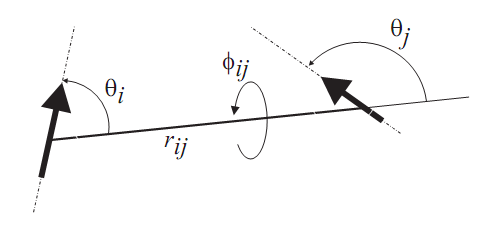
\includegraphics[width=0.55\columnwidth]{fig_Schematic-of-the-angles.png}
	\caption{Schematic of the angles between two point dipoles $i$ and $j$ indicated by the arrows, which are situated
		on different molecules at a distance $r_{ij}$.}
	\label{fig:Schematic-of-the-angles}
\end{figure}
\newline \newline
\textbf{Linear point quadrupole.} A linear point quadrupole describes the electrostatic field induced either by two
collinear point dipoles with the same moment, but opposite orientation at a distance $a \rightarrow 0$, or by at least
three collinear point charges with alternating sign $\left(q, -2q, q\right)$. The resulting quadrupole moment $Q$ is defined by $Q=2aq$. The electrostatic interaction between two linear point quadrupoles with the moments $Q_{i}$ and $Q_{j}$ at a
distance $r_{ij}$ is given by \cite{gray, hirschfelder}
\begin{eqnarray}
u^{QQ}_{ij}\left(r_{ij}, \theta_{i}, \theta_{j}, \phi_{ij}, Q_{i}, Q_{j}\right) & = & \frac{1}{4 \pi \epsilon_{0}}\frac{3}{4} \frac{Q_{i}Q_{j}}{r^{5}_{ij}} \nonumber \\ 
& & [1-5 (\left(\cos \theta_{i}\right)^2 + \left(\cos \theta_{j}\right)^{2}) - 15\left(\cos \theta_{i}\right)^{2}\left(\cos \theta_{j}\right)^{2}+ \nonumber \\ 
& & 2\left(\sin \theta_{i} \sin \theta_{j} \cos \phi_{ij} - 4 \cos \theta_{i} \cos \theta_{j}\right)^{2}] \;,
\end{eqnarray}
where the angles $\theta_{i}$, $\theta_{j}$ and $\phi_{ij}$ indicate the relative angular orientation of the two point quadrupoles, as discussed above. Note that no long range correction is necessary for this interaction type if the fluid is isotropic.
\newline \newline
\textbf{Point dipole interactions.} The interaction between a point dipole with moment $\mu_{i}$ and a point charge $q_{j}$ at a distance $r_{ij}$ is given by \cite{hirschfelder, lorrain}
\begin{equation}
u^{Dq}_{ij}\left(r_{ij}, \theta_{i}, \mu_{i}, q_{j}\right)=-\frac{1}{4\pi \epsilon_{0}} \frac{\mu_{i} q_{j}}{r^{2}_{ij}} \cos \theta_{i} \;.
\label{eq:PointDipoleInteractions}
\end{equation}
Here, $\theta_{i}$ is the angle between the distance vector of the point charge and the orientation vector of the point dipole, as illustrated in Figure~\ref{fig:Schematic-of-the-angles}.
\newline \newline
\textbf{Point quadrupole interactions.} The interaction potential of a linear point quadrupole $Q_{i}$ with a point charge $q_{j}$ at a distance $r_{ij}$ is given by \cite{allen, gray}
\begin{equation}
u^{Qq}_{ij}\left(r_{ij},\theta_{i},Q_{i},q_{j}\right)=\frac{1}{4\pi \epsilon_{0}} \frac{Q_{i}q_{j}}{4 r^{3}_{ij}}\left(3\cos^{2}\theta_{i}-1\right) \;,
\label{eq:PointQuadrupoleInteractionsPointCharge}
\end{equation}
where $\theta_{i}$ is the angle between the distance vector of the point charge and the orientation vector of the point
quadrupole, as illustrated in Figure~\ref{fig:Schematic-of-the-angles}.

The interaction between a linear point quadrupole with moment $Q_{i}$ and a point dipole with moment $\mu_{j}$ is given
by \cite{gray, hirschfelder}
\begin{eqnarray}
u^{Q\mu}_{ij}\left(r_{ij},\theta_{i},\theta_{j},\phi_{ij},Q_{i},\mu_{j}\right) & = & \frac{1}{4\pi\epsilon_{0}}\frac{3}{2}\frac{Q_{i}\mu_{j}}{r^{4}_{ij}}\left(\cos \theta_{i}-\cos \theta_{j}\right) \nonumber \\
& & \left(1+3\cos \theta_{i} \cos \theta_{j}-2\cos \phi_{ij} \sin \theta_{i} \sin \theta_{j}\right) \;,
\label{eq:PointQuadrupoleInteractionsPointDipole}
\end{eqnarray}
where the angles $\theta_{i}$, $\theta_{j}$ and $\phi_{ij}$ indicate the relative angular orientation of the point dipole $j$ and the point quadrupole $i$, as shown in Figure~\ref{fig:Schematic-of-the-angles}.
\newline \newline



\subsection{Intramolecular Interactions}
\label{sec:Intramolecular Interactions}
% Michael


\subsection{Mixing rules}
\label{sec:Mixing rules}
% Simon


For pure components, the interactions between two different LJ sites are described by the Lorentz-Berthelot
combination rules \cite{berthelot, lorentz}. For mixtures, the combination rules are extended to the modified Lorentz-Berthelot
rules, which include two additional parameters $\eta$ and $\xi$ to describe the interactions between LJ sites of unlike
molecules \cite{fischer}
\begin{eqnarray}
\sigma_{ij} &=& \eta\frac{\sigma_{i}+\sigma_{j}}{2} \;, \\
\epsilon_{ij} &=& \xi\sqrt{\epsilon_{i}\epsilon_{j}} \;.
\end{eqnarray}
The two parameters scale all LJ interactions between molecules of different components equally. Arbitrary
modifications of the combination rules are possible. \textit{ms}2 allows the specification of $\eta$ and $\xi$ for every molecule pair independently and thus the free parameterization of the combination rules.


\section{Cutoff \& long range correction}
\label{sec:Cutoff long range correction}
% 


\subsection{Reaction Field}
\label{sec:Reaction Field}
% 

\textbf{Reaction field method.} The truncation of interactions between first and second order electrostatic sites leads to
errors that need to be corrected. The reaction field method \cite{frenkel, nymand} is implemented in \textit{ms}2 for this task, being widely used and well accepted \cite{steinhauser, vanderSpoel}. Its advantages are accuracy and stability, while requiring little computational effort compared to other techniques like Ewald summation \cite{ewald}. However, it is limited to electro-neutral
systems, thus \textit{ms}2 is currently restricted to electro-neutral molecules. The basic assumption of the reaction field
method implemented in \textit{ms}2 is that the system is sufficiently large so that tinfoil boundary conditions $\left(\epsilon_{s} \rightarrow \infty\right)$
are applicable without a loss of accuracy. This is the case for $N\geq 500$ \cite{lisal, garzon, lisal1, jedlovszky}.

All dipoles within the cut-off radius $r_{\text{c}}$ polarize the fluid surrounding the cut-off sphere,
which is modeled as a dielectric continuum with a relative permittivity $\epsilon_{s}$. The polarization gives rise to a
homogeneous electric field within the cut-off radius, called the reaction field $\textbf{\textit{E}}^{\text{RF}}_{i}$ of magnitude
\begin{equation}
\textbf{\textit{E}}^{\text{RF}}_{i}=\frac{1}{4\pi \epsilon_{0}} \frac{2\left(\epsilon_{s}-1\right)}{2\epsilon_{s}+1} \frac{1}{r^{3}_{\text{c}}} \sum^{m}_{b=1} \sum_{j=1 \atop r_{ij}<r_{\text{c}}}^{N_{b}} \boldsymbol \mu_{b,j} \;.
\label{eq:ReactionFieldMethod}
\end{equation}
Note that all $m$ dipoles with moment $\boldsymbol \mu$ on all $N_{b}$ molecules within the cut-off sphere have to be summed up.
The reaction field acting outside of the cut-off sphere interacts with a dipole $\boldsymbol \mu_{i}$ at the center of the cut-off sphere by \cite{allen, boettcher}
\begin{equation}
u_{i}^{\mu \text{RF}}=- \frac{1}{2} \boldsymbol \mu_{i} \textbf{\textit{E}}_{i}^{\text{RF}} \;,
\label{eq:ReactionFieldMethodContribution}
\end{equation}
where $u_{i}^{\mu \text{RF}}$ is its contribution to the potential energy. Eq.~\eqref{eq:ReactionFieldMethodContribution} makes use of the assumption that the system is sufficiently large.

The reaction field method can also be applied to correct for sets of point charges, as long as they add up to a total
charge of zero. Therefore, a point charge distribution is reduced to a dipole vector $\boldsymbol \mu^{q}$ according to
\begin{equation}
\boldsymbol \mu^{q}=\sum^{n}_{i=1} \boldsymbol r_{i} q_{i} \;,
\label{eq:ReactionFieldMethodPointCharges}
\end{equation}
where $n$ denotes the total number of point charges and $\boldsymbol r_{i}$ the position vector of charge $q_{i}$. The resulting dipole $\boldsymbol \mu^{q}$ is transferred into the correction term according to Eqs.~\eqref{eq:ReactionFieldMethod} and~\eqref{eq:ReactionFieldMethodContribution}.


\subsection{Ewald summation}
\label{sec:Ewald summation}
% 

Ewald summation~\cite{allen1987, frenkel2003} was implemented for the calculation of electrostatic interactions between point charges. It extends the applicability of $ms$2 to thermodynamic properties of e.g. ions in solutions. In Ewald summation, the electrostatic interactions according to Coulomb's law are divided into two contributions: short-range and long-range. The short-range term includes all charge-charge interactions at distances smaller than the cut-off radius. The remaining contribution is calculated in Fourier space and only the final value is transformed back into real space. This allows for an efficient calculation of the long-range interactions between the charges. The algorithm is well described in literature. Currently, some of the new features, the calculation of Massieu potential derivatives and Hybrid MPI \& OpenMP Parallelization for MD, are not available together with Ewald summation.

% in ms2par ist auch "Rodgers" auswählbar!?!?

\section{Computing physical properties}
\label{sec:PhysProps}

\subsection{Ensembles Overview}
\label{sec:Ensembles}

An ensembles is the set of all theoretically possible configurations (states) under some specific macroscopic conditions. For example, the canonical ensemble ($NVT$) is the set of all configurations that fulfills the condition of having the same temperature $T$, volume $V$ and number of particles $N$, whereas the isobaric-isothermal ensemble ($NpT$) represents a system at constant temperature $T$, pressure $p$, and number of particles $N$. Independent on the specific macroscopic conditions, an MC simulation always involve the creation of a trial configuration according to some probability $\alpha_{ij}$, where $i$ refers to the previous state of the system, while $j$ refers to the new one generated with $\alpha_{ij}$ probability from $i$. Another probability, $a_{ij}$, determines that the newly generated state $j$ is actually accepted as a proper configuration of the specific ensemble or not. Thus, the transition probability between state $i$ and $j$ is $\pi_{ij}=\alpha_{ij} a_{ij}$. The transition probability for state $i$ depends only on the previous state $j$. This property is called the Markov chain property; the sequence of configurations created by this way is defined as the Markov chain. It can be shown that if a Markov chain satisfies the condition $P_i \pi_{ij}=P_j \pi_{ji}$ (for every state $i$ and $j$) of \textit{microscopic reversibility} then the probability of every configuration in the Markov chain will converge to the arbitrarily chosen set of probabilities $\textbf{P}=[P_1,P_2,...,P_i,...]$ as the length of the chain increases. Once \textbf{P} is specified, the microscopic reversibility condition $P_i \pi_{ij}=P_j \pi_{ji}$ can be solved and has potentially more than one solution for $a_{ij}$. A solution for $a_{ij}$ is called the acceptance criterion of the ensemble. The generation of the next potential configuration is done such a way that $\alpha$ is symmetric, i.e. $\alpha_{ij}=\alpha_{ji}$. This way $\alpha_{ij}$ and $\alpha_{ji}$ cancel each other in the equation. It is sensible to specify $\textbf{P}=[P_1,P_2,...,P_i,...]$ as the set of actual probability of occurrence of the configurations $1,2,...,i,...$ in the ensemble.\\
With the exception of the $NVE$ ensemble, not every theoretically possible configuration of an ensemble has the same probability of occurrence. In fact, only a small subset of configurations is truly relevant even though the set of all theoretically possible configurations of an ensemble is extremely large. Although, the analytical form of $P_i$ is known for an ensemble, its numerical value is not. Therefore, the way of calculating a macroscopic property $A$ as an \textit{ensemble average} using the standard statistical formula for the expected value $<A>=\sum A_i P_i$ (for every possible $i$), where $A_i$ is the value of property $A$ for configuration $i$, is not feasible. However, it can be shown that if configurations are selected randomly (\textit{Monte Carlo sampling}) and selected according to their actual probability of occurrence $P_i$ at the same time (\textit{importance sampling}) then the expected value can be calculated as $<A>=\sum A_i/n$ (assuming the number of sampled configurations $n$ is large enough). A Markov chain satisfying the microscopic reversibility criterion $P_i \pi_{ij}=P_j \pi_{ji}$ fulfills exactly this condition, because it selects $n$ configurations according to their actual probability of occurrence $P_i$.
 
Following type of simulations are currently supported by \textit{ms}2:
\begin{itemize}
	\item canonical ensemble ($NVT$) MC (corresponds to MD with thermostat)
	\item micro-canonical ensemble ($NVE$) MC (corresponds to MD)
	\item isobaric-isothermal ensemble ($NpT$) MC (corresponds to MD with thermostat and barostat)
	\item grand equilibrium method (pseudo-$\mu VT$) MC (MC only)
\end{itemize}

For the micro-canonical ensemble, the MC acceptance criterion for molecular translation and rotation is 
\begin{equation}
\mathrm{min}\left(1, \frac{(E-U_j)^{(F-2)/2} \mathrm{\theta(E-U_j)}}{(E-U_i)^{(F-2)/2} \mathrm{\theta(E-U_i)}} \right) ,
\label{eq:acccritNVE}
\end{equation}
where $E$ is the total \textit{hamiltonian} of the system that is a sum of the total kinetic $K$ and potential energy $U$ of the system, $F$ is the sum of the individual molecular degrees of freedom in the system, and $\theta$ is the unit step function \cite{Lus98}.
The MC acceptance criterion for the canonical ensemble for molecular translation and rotation is 
\begin{equation}
\mathrm{min}\left(1, \mathrm{exp}(-\beta(U_j-U_i)) \right),
\label{eq:acccritNVT}
\end{equation}
where $\beta$ is the inverse temperature.\\

For the $NpT$ ensemble, the MC acceptance criterion for molecular translation and rotation as well as volume change is
\begin{equation}
\text{min}\left(1, \text{exp}( -\beta(U_j-U_i+p(V_j-V_i))+N\text{ln}(V_j/V_i) )  \right).
\label{eq:acccritNVT}
\end{equation}

\subsection{Statistical uncertainties}
\label{sec:Statun}

The simulation program \textit{ms}2 calculates the thermodynamic properties from the trajectories (MD) or Markov Chains (MC) on the fly. The results are written to file with a specified frequency during the course of the simulation. The statistical uncertainties of all results are estimated using the block averaging method according to Flyvbjerg and Petersen \cite{flyvberg} and the error propagation law.

\subsection{Static properties from Helmholtz free energy derivatives (NVT, NVE)}
\label{sec:PropHelm}

Standard textbook approaches in the molecular simulation literature indicate specific statistical mechanical ensembles for particular thermodynamic properties. E.g., properties originating from differentiation with respect to temperature at constant pressure, such as the isothermal compressibility, are most likely considered to be candidates for the $NpT$ ensemble, while for a property such as the isochoric heat capacity, the $NVT$ ensemble is considered to be a natural choice. It is true that certain properties have simpler statistical analogs in certain ensembles and may be difficult to derive in other ensembles. Fundamentally, however, the above mentioned philosophy misleading. In principle, any thermodynamic property is accessible in any ensembles. The formalism proposed by Lustig ~\cite{Lus11, Lus12} allows for the calculation of an arbitrary number of derivatives
\begin{align} 
A^\mathrm{r}_{nm}=(1/T)^n \rho^m \frac{\partial^{n+m}f^\text{r}(T,\rho)/(RT)}{\partial(1/T)^n \partial \rho^m}
\label{eq:helmholtzderiv}
\end{align}
for $n>0$ or $m>0$ in the $NVT$ and $NVE$ ensembles, with the molar residual Helmholtz energy $f$, the temperature $T$, the density $\rho$, the molar gas constant $R$. It can be shown that the total $f/(RT)$ can be additively separated into an ideal $f^\text{o}/(RT)$ and a residual part$f^\text{r}/(RT)$. The ideal part by definition corresponds to the value of $f/(RT)$ when no intermolecular interactions are at work \cite{SpanBook}. $f^\text{o}/(RT)$ consist of an exclusively temperature and an exclusively density dependent part. The former has a trivial density dependence $\ln(\rho/\rho_\text{ref})$, whereas the latter has a non-trivial temperature dependence.\\
The approach is based on the fact that the fundamental equation of state contains the complete thermodynamic information about a system, which can be expressed in terms of various thermodynamic potentials~\cite{MunsterBook}, e.g. internal energy $E(N,V,S)$, enthalpy $H(N,p,S)$, Helmholtz free energy $F(N,V,T)$ or Gibbs free energy $G(N,p,T)$, with number of particles $N$, volume $V$, pressure $p$, temperature $T$ and entropy $S$. These representations are equivalent in the sense that any other thermodynamic property is essentially a combination of derivatives of the chosen form with respect to its independent variables. The form $f/(RT)(N,V,1/T)$, known as the Massieu potential, is preferable due to practical reasons. Namely, neither its independent variables nor its derivatives with respect these variables involve entropic properties. Moreover, some of its derivatives are directly related to measurable properties.\\
Since $f$ is a thermodynamic potential, any other static thermodynamic property is a combination of its partial derivatives. The molar internal energy $u$, pressure $p$, molar enthalpy $h$, molar Gibbs energy $g$, and molar isochoric heat capacity $c_v$ are simple functions
\begin{align}
\frac{u}{RT}=A^\text{o}_{10}(T)+A^\text{r}_{10},
\label{eq:internalen}
\end{align}
\begin{align}
\frac{p}{\rho RT}=1+A^\text{r}_{01},
\label{eq:pressure}
\end{align}
\begin{align}
\frac{1}{RT}\left(\frac{\partial p}{\partial \rho}\right)_T=1+2A^\text{r}_{01}+A^\text{r}_{02},
\label{eq:dpdrho}
\end{align}
\begin{align}
\frac{1}{\rho{R}}\left(\frac{\partial p}{\partial T}\right)_\rho=1+A^\text{r}_{01}-A^\text{r}_{11},
\label{eq:dpdt}
\end{align}
\begin{align}
\frac{h}{RT}=1+A^\text{r}_{01}+A^\text{o}_{10}(T)+A^\text{r}_{10},
\label{eq:enthalpy}
\end{align}
\begin{align}
\frac{g}{RT}=1+A^\text{r}_{01}+A^\text{o}_{00}+A^\text{r}_{00},
\label{eq:gibbs}
\end{align}
\begin{align}
\frac{c_v}{R}=-A^\text{o}_{20}(T)-A^\text{r}_{20},
\label{eq:cv}
\end{align}
while molar isobaric heat capacity $c_p$, and speed of sound $w$ are non-linear combinations of derivatives
\begin{align}
\frac{c_p}{R}=-A^\text{o}_{20}(T)-A^\text{r}_{20}+\frac{(1+A^\text{r}_{01}-A^\text{r}_{11})^2}{1+2A^\text{r}_{01}+A^\text{r}_{02}},
\label{eq:cp}
\end{align}
\begin{align}
\frac{Mw^2}{RT}=1+2A^\text{r}_{01}+A^\text{r}_{02}-\frac{(1+A^\text{r}_{01}-A^\text{r}_{11})^2}{A^\text{o}_{20}(T)+A^\text{r}_{20}},
\label{eq:sos}
\end{align}
where $M$ is the molar mass, $A^\text{r}_{nm}=A^\text{r}_{nm}(T, \rho)$, and $A^\text{o}_{nm}=A^\text{o}_{nm}(T, \rho)=(1/T)^n \rho^m \cdot \partial^{n+m}[\alpha^\text{o}(T)+\alpha^\text{o}(\rho)]/\partial(1/T)^n / \partial \rho^m =A^\text{o}_{nm}(T)+A^\text{o}_{nm}(\rho)$. Note that the ideal part
\begin{itemize}
	\item $A^\text{o}_{nm}(T, \rho)=0$, for $n>0$ and $m>0$,
	\item $A^\text{o}_{nm}(T, \rho)=A^\text{o}_{nm}(T)+0$, for $n>0$ and $m=0$,
	\item $A^\text{o}_{nm}(T, \rho)=0+(-1)^{1+m}$, for $n=0$ and $m>0$.
\end{itemize}
A more complete list of thermodynamic properties can be found in Ref. \cite{SpanBook}. For the $NVE$ ensemble, there are two sets of $A^\text{r}_{nm}$ output values in $ms$2. Each set corresponds to a different statistical mechanical entropy definition \cite{Lus12}. The numerical values for these definitions should converge to the same number as the system size increases and they should be identical in the thermodynamic limit $(N \rightarrow \infty)$.\\

The $A^\text{r}_{nm}$ derivatives are determined from fluctuation formulas. These fluctuation formulas require the ensemble average of $U^n$ and ${\partial^m U}/{\partial V^m}$ with respect to the applied molecular interaction pair potential. Thus the explicit analytical expressions for $U^n$ and ${\partial^m U}/{\partial V^m}$ have to be determined analytically beforehand ~\cite{Lus11, Lus12}. The general formula for ${\partial^m U}/{\partial V^m}$ can be found in Ref. ~\cite{Lus94b}. For common molecular interaction pair potentials, like the Lennard-Jones potential~\cite{allen}, describing repulsive and dispersive interactions, or Coulomb's law, describing electrostatic interactions between point charges, the explicit analytical formulas can be obtained straightforwardly. The mathematical form of the long range correction (LRC) for $U$ and ${\partial^m U}/{\partial V^m}$ depends on the molecular interaction potential and the cut-off method (site-site or center-of-mass cut-off mode) applied. For the Lennard-Jones potential, the LRC scheme was well described in the literature for both the site-site~\cite{Lus11, Mei06} and the center of mass cut-off mode~\cite{Lus94b, Lus88}. For the usual implementation of the reaction field method ~\cite{RFmethod, siteRFmethod}, the LRC for ${\partial^m U}/{\partial V^m}$ can be obtained straightforwardly. However, practical applications show that the electrostatic LRC of ${\partial U}/{\partial V}$ and ${\partial^2 U}/{\partial V^2}$ can be neglected in case of systems for which the reaction field method is an appropriate choice. E.g., the contribution of the electrostatic LRC for a liquid system ($T=298$ K and $\rho= 45.86$ mol/l) consisting of only 200 water and 50 methanol molecules with a very short cut-off radius of $20\%$ of the edge length of the simulation volume is still $<<1\%$ for both ${\partial U}/{\partial V}$ and ${\partial^2 U}/{\partial V^2}$.\\

The supplementary material of Ref. ~\cite{ms2release2.0} contains the explicit fluctuation formulas as well as the LRC contributions with respect to the implemented molecular interaction pair potentials in $ms$2 for the $A^\text{r}_{nm}$ derivatives up to the order of $n=3$ and $m=2$.

\subsection{Static properties from conventional fluctuation formulas (NpT, NpH)}
\label{sec:PropConv}

Several static thermodynamic properties have simple statistical analogs in certain ensembles.\\

%At constant temperature and volume ($NVT$ ensemble), e.g. the pressure is determined by the virial expression $W$. Other important
%thermodynamic properties are accessible at constant temperature and pressure. In the $NpT$ ensemble, the volume is a fluctuating %parameter that on average yields the volume corresponding to the specified temperature and
%pressure. In both ensembles, the residual internal energy is the sum of all pairwise interaction energies $u_{ij}$ and
%the appropriate long range correction. The residual enthalpy is linked to the residual internal energy, pressure
%and volume of the system using the thermodynamic definition.

%At constant temperature $T$ and volume $V$, the pressure $p$ is determined by \cite{allen}
%\begin{equation}
%p=\frac{k_{\text{B}}T}{V}+\frac{\left\langle W\right\rangle}{V}+\Delta p^{L}=\frac{k_{\text{B}}T}{V}+\frac{1}{3V}\left\langle %\sum^{N-1}_{i=1}\sum_{j=i+1\atop r_{ij}<r_{\text{c}}}^{N} \textbf{\textit{r}}_{ij}\textbf{\textit{f}}_{ij}\right\rangle +\Delta %p^{L} \;,
%\label{eq:pressure}
%\end{equation}
%where $k_{\text{B}}$ is the Boltzmann constant and the brackets $\left\langle \ldots \right\rangle$ indicate the ensemble average. $W$ denotes the virial,
%which is defined by the force vector $\textbf{\textit{f}}_{ij}$ acting between two molecules at a separation vector %$\textbf{\textit{r}}_{ij}$ between their centers of mass. The contribution $\Delta p^{L}$ considers the long-range interactions with %molecules beyond the cut-off radius $r_{\text{c}}$.

%In the $NpT$ ensemble, the volume is a fluctuating parameter that on average yields the volume
%corresponding to the specified pair of temperature $T$ and pressure $p_{0}$. In MD simulations with Andersen's
%barostat \cite{andersen}, which is implemented in \textit{ms}2, the fluctuations of the volume are damped by a fictive piston mass %$Q_{\text{p}}$ according to the equation of motion
%\begin{equation}
%\ddot{V}=\frac{p-p_{0}}{Q_{\text{p}}} \;.
%\label{eq:fictivepistonmass}
%\end{equation}
%In MC simulations, the volume is changed randomly and the new volume accepted by applying the Metropolis
%acceptance criterion
%\begin{equation}
%P_{acc}=\text{min} \left(1, \exp \left(\frac{\Delta E}{k_{\text{B}}T}\right)\right) \;,
%\label{eq:metropolisacceptancecriterion}
%\end{equation}
%where $P_{acc}$ is the probability of accepting the volume change and $\Delta E$ is the difference between the old state with
%energy $U_{old}$ for the volume $V_{old}$ and the new state with energy $U_{new}$ for the volume $V_{new}$ according to
%\begin{equation}
%\Delta E=p_{0}\left(V_{new}-V_{old}\right)+\left(U_{new}-U_{old}\right)+Nk_{\text{B}}T \ln \frac{V_{old}}{V_{new}} \;.
%\label{eq:differencestate}
%\end{equation}

%The residual enthalpy $H^{\text{res}}$ is directly linked to the residual internal energy, pressure and volume of the system
%\begin{equation}
%H^{\text{res}}=U^{\text{res}}+pV-Nk_{\text{B}}T \;,
%\label{eq:enthalpy}
%\end{equation}
%where $U^{\text{res}}$ is the residual potential energy. It is defined as the sum of all pairwise interaction energies $u_{ij}$ and
%the appropriate long range correction $\Delta U^{L}$, cf. section 5.5
%\begin{equation}
%U^{\text{res}}=\sum^{N-1}_{i=1} \sum_{j=i+1\atop r_{ij}<r_{\text{c}}}^{N} u_{ij} + \Delta U^{L} \;.
%\label{eq:internalenergy}
%\end{equation}


%The accessible second derivatives vary with the employed ensemble. In the $NVT$ ensemble, the residual
%isochoric heat capacity $c^{res}_{v}$ is determined by fluctuations of the residual potential energy $U^{\text{res}}$
%\begin{equation}
%c^{\text{res}}_{v}=\frac{1}{N} \left(\frac{\partial U^{\text{res}}}{\partial %T}\right)_{v}=\frac{1}{k_{\text{B}}\left(NT\right)^{2}}\left(\left\langle \left(U^{\text{res}}\right)^{2}\right\rangle - %\left\langle U^{\text{res}}\right\rangle ^{2}\right) \;.
%\label{eq:isochoricheatcapacity}
%\end{equation}
%The partial derivative of the potential energy with respect to the volume at constant temperature $(\partial U^{\text{res}}/ %\partial V)_{T}$ is determined by fluctuations of the residual potential energy $U^{\text{res}}$ and the virial $W$
%\begin{equation}
%\left(\frac{\partial U^{\text{res}}}{\partial V}\right)_{T}=\frac{N}{3V} \left(\frac{1}{k_{\text{B}}T}\left(\left\langle %W\right\rangle \left\langle U^{\text{res}}\right\rangle - \frac{1}{N} \left\langle WU^{\text{res}}\right\rangle\right)+\left\langle %W\right\rangle \right) \;.
%\label{eq:partialderivativeofthepotentialenergy}
%\end{equation}

In the $NpT$ ensemble, the second derivatives of the Gibbs energy, namely the residual isobaric heat capacity $c^{\text{res}}_{p}$, the isothermal compressibility $\beta_{T}$ and the volume expansivity $\alpha_{p}$ are functions of ensemble fluctuations \cite{allen}. The residual isobaric heat capacity $c^{\text{res}}_{p}$ is related to fluctuations of the residual enthalpy $H^{\text{res}}$
\begin{equation}
c^{\text{res}}_{p}=\frac{1}{N} \left(\frac{\partial H^{\text{res}}}{\partial T}\right)_{p} = \frac{1}{k_{\text{B}}\left(NT\right)^{2}} \left(\left\langle \left(H^{\text{res}}\right)^{2}\right\rangle-\left\langle H^{\text{res}}\right\rangle ^{2}\right) \;.
\label{eq:isobaricheatcapacity}
\end{equation}
To obtain the total isobaric heat capacity $c_{p}$, the solely temperature dependent ideal gas contribution $c^{\text{id}}_{p}\left(T\right)$ has to be added. This ideal property is accessible e.g. by quantum chemical methods and can often be found in data bases \cite{rowley}.

An analogous relationship links the isothermal compressibility $\beta_{T}$ to volume fluctuations in the $NpT$ ensemble
\begin{equation}
\beta_{T}=-\frac{1}{V}\left(\frac{\partial V}{\partial p}\right)_{T}=\frac{1}{k_{\text{B}}T\left\langle V\right\rangle} \left(\left\langle V^{2}\right\rangle - \left\langle V\right\rangle ^{2}\right) \;.
\label{eq:isothermalcompressibility}
\end{equation}
The partial derivative of the residual enthalpy with respect to the pressure at constant temperature $(\partial H^{\text{res}}/ \partial p)_{T}$ is linked to fluctuations of volume and residual internal energy
\begin{equation}
\left(\frac{\partial H^{\text{res}}}{\partial p}\right)_{T}=V-\frac{N}{T}\left(\left\langle U^{\text{res}}V\right\rangle - \left\langle U^{\text{res}}\right\rangle\left\langle V\right\rangle+p\left(\left\langle V^{2}\right\rangle-\left\langle V\right\rangle ^{2}\right)\right) \;,
\label{eq:derivativeoftheresidualenthalpy}
\end{equation}
and the volume expansivity $\alpha_{p}$ again to volume and residual enthalpy fluctuations
\begin{equation}
\alpha_{p}=\frac{1}{V}\left(\frac{\partial V}{\partial T}\right)_{p}=\frac{N}{T^{2}\left\langle V\right\rangle}\left(\left\langle H^{\text{res}}V\right\rangle-\left\langle H^{\text{res}}\right\rangle\left\langle V\right\rangle\right) \;.
\label{eq:volumeexpansivity}
\end{equation}

The speed of sound $w$ is the velocity of a sound wave traveling through an elastic medium. It can be given by the
isothermal compressibility $\beta_{T}$, the volume expansivity $\alpha_{p}$, the isobaric heat capacity $c_{p}$ and the temperature $T$ by
\begin{equation}
w=\left(\frac{1}{M\left(\beta_{T}\rho-T\alpha^{2}_{p}/c_{p}\right)}\right)^{0.5} \;,
\label{eq:speedofsound}
\end{equation}
where $M$ is the molar mass. In \textit{ms}2, the speed of sound is calculated both for pure components and mixtures in the $NpT$ ensemble.

\subsection{Transport properties}
\label{sec:Transport properties}
% Tatjana

In \textit{ms}2, transport properties are calculated using equilibrium MD. Here, the fluctuations of a system around
its equilibrium state are evaluated as a function of time. The Green-Kubo formalism relates these microscopic
fluctuations to the respective transport properties.
\newline \newline
\textbf{Diffusion coefficients.} The self-diffusion coefficient $D_{i}$ is related to the mass flux of single molecules within a fluid. Therefore, the relevant Green-Kubo expression is based on the individual molecule velocity autocorrelation
function \cite{gubbins1}
\begin{equation}
D_{i}=\frac{1}{3N_{i}}\int^{\infty}_{0} \mathrm dt \left\langle \textbf{v}_{k}\left(t\right) \cdot \textbf{v}_{k}\left(0\right)\right\rangle \;,
\label{eq:selfdiffusioncoefficient}
\end{equation}
where $\textbf{v}_{k}\left(t\right)$ is the center of mass velocity vector of molecule $k$ at some time $t$. Eq.~\eqref{eq:selfdiffusioncoefficient} is an average over all $N_{i}$ molecules of component $i$ in the ensemble, since all contribute to the self-diffusion coefficient. In binary mixtures, the Maxwell-Stefan diffusion coefficient $\dcoeff_{ij}$ is defined by \cite{krishna}
\begin{equation}
\dcoeff_{ij}=\frac{x_{j}}{x_{i}}\Lambda_{ii}+\frac{x_{i}}{x_{j}}\Lambda_{jj}-\Lambda_{ij}-\Lambda_{ji} \;,
\label{eq:diffusioncoefficient}
\end{equation}
where $x_{i}=N_{i}/N$ and $\Lambda_{ij}$ can be written in terms of the center of mass velocity
\begin{equation}
\Lambda_{ij}=\frac{1}{3N} \int^{\infty}_{0} \mathrm dt \left\langle \sum^{N_{i}}_{k=1} \textbf{v}_{i,k}\left(0\right) \cdot \sum^{N_{j}}_{l=1} \textbf{v}_{j,l} \left(t\right)\right\rangle \;.
\label{eq:difcoef}
\end{equation}
From the expressions above, the collective character of the Maxwell-Stefan diffusion coefficient is evident. This
leads to significantly less data for a given system size and time step and therefore to larger statistical uncertainties
than in case of the self-diffusion coefficient. Note that equations for the Maxwell-Stefan diffusion coefficient are
implemented in \textit{ms}2 both for binary and ternary mixtures \cite{krishna}.
\newline \newline
\textbf{Shear viscosity.} The shear viscosity $\eta$, as defined by Newton's "law" of viscosity, is a measure of the resistance of a fluid to a shearing force \cite{hoheisel}. It is associated with the momentum transport under the influence of velocity
gradients. Hence, the shear viscosity can be related to the time autocorrelation function of the off-diagonal
elements of the stress tensor $\textbf{J}_{p}$ \cite{gubbins1}
\begin{equation}
\eta=\frac{1}{Vk_{\text{B}}T} \int^{\infty}_{0} \mathrm dt \left\langle J^{xy}_{p}\left(t\right) \cdot J^{xy}_{p}\left(0\right)\right\rangle \;.
\label{eq:shearviscosity}
\end{equation}
Averaging over all three independent elements of the stress tensor, i.e. $J^{xy}_{p}$, $J^{xz}_{p}$ and $J^{yz}_{p}$, improves the statistics.
The component $J^{xy}_{p}$ of the microscopic stress tensor $\textbf{J}_{p}$ is given in terms of the molecular positions and velocities by \cite{hoheisel}
\begin{equation}
J^{xy}_{p}=\sum^{N-1}_{i=1} mv^{x}_{i}v^{y}_{i}-\sum^{N-1}_{i=1}\sum^{N}_{j=i+1}\sum^{n}_{k=1}\sum^{n}_{l=1} r^{x}_{ij} \frac{\partial u_{ij}}{\partial r^{y}_{kl}} \;.
\label{eq:componentofstresstensor}
\end{equation}
Here, the lower indices $l$ and $k$ indicate the $n$ interaction sites of a molecule and the upper indices $x$ and $y$ denote
the spatial vector components, e.g. for velocity $v^{x}_{i}$ or site-site distance $r^{x}_{ij}$. The first term of Eq.~\eqref{eq:componentofstresstensor} is the kinetic energy contribution and the second term is the potential energy contribution to the shear viscosity. Consequently, the Green-Kubo integral~\eqref{eq:shearviscosity} can be decomposed into three parts, i.e. the solely kinetic energy contribution, the solely potential energy contribution and the mixed kinetic-potential energy contribution \cite{hoheisel}.
\newline \newline
\textbf{Bulk viscosity.} The bulk viscosity $\eta_{v}$ refers to the resistance to dilatation of an infinitesimal volume element at constant shape \cite{barton}. The bulk viscosity can be calculated by integration of the time-autocorrelation function
of the diagonal elements of the stress tensor and an additional term that involves the product of pressure $p$ and
volume $V$, which does not appear in the shear viscosity, cf. Eq.~\eqref{eq:shearviscosity}. In the $NVE$ ensemble, the bulk viscosity
is given by \cite{gubbins1, steele}
\begin{equation}
\eta_{v}=\frac{1}{Vk_{\text{B}}T} \int^{\infty}_{0} \mathrm dt \left\langle \left(J^{xx}_{p}\left(t\right)-pV\left(t\right)\right) \cdot \left(J^{xx}_{p}\left(0\right)-pV\left(0\right)\right)\right\rangle \;.
\label{eq:bulkviscosity}
\end{equation}
The diagonal component $J^{xx}_{p}$ of the microscopic stress tensor $\textbf{J}_{p}$ is defined analogous to Eq.~\eqref{eq:componentofstresstensor}. The statistics of the ensemble average in Eq.~\eqref{eq:bulkviscosity} can be improved using all three independent diagonal elements of the stress
tensor $J^{xx}_{p}$, $J^{yy}_{p}$ and $J^{zz}_{p}$. Eqs.~\eqref{eq:componentofstresstensor} and~\eqref{eq:bulkviscosity} can directly be applied for mixtures.

\textbf{electric conductivity}
The evaluation of the electric conductivity $\sigma$ was implemented in $ms$2 version 2.0, being a measure for the flow of ions in solution. The Green-Kubo formalism~\cite{gubbins1972} offers a direct relationship between $\sigma$ and the time-autocorrelation function of the electric current flux $\bm{j_e}(t)$ ~\cite{HansenBook}
\begin{equation}
\sigma=\frac{1}{3Vk_{\mathrm{B}}T}\int_0^{\infty}~\big\langle \bm{j_e}(t)\cdot \bm{j_e}(0) \big\rangle  \mathrm{d} t \mbox{   ,}
\label{Erdalkali_elcond}
\end{equation}
where $k_\texttt{B}$ is Boltzmann’s constant. The electric current flux is defined by the charge $q_k$ of ion $k$ and its velocity vector $\bm{v}_k$ according to
\begin{equation}
\bm{j_e}(t)=\sum_{k=1}^{N_{j}} q_k \cdot \bm{v}_{k}(t) \mbox{   ,}
\label{elflux}
\end{equation}
where $N_{j}$ is the number of molecules of component $j$ in solution. Note that only the ions in the solution have to be considered, not the electro-neutral molecules.
For better statistics, $\sigma$ is sampled over all independent spatial elements of $\bm{j_e}(t)$.



\textbf{thermal conductivity}
In the previous version of $ms2$ the determination of the thermal conductivity by means of the Green-Kubo formalism was implemented for pure substances only. In the present release, the calculation of the thermal conductivity was extended to multi-component mixtures. The thermal conductivity $\lambda$ is given by the autocorrelation function of the elements of the microscopic heat flow ${J}^{x}_{q}$
\begin{equation}\label{themalcond}
\lambda=\frac{1}{Vk_BT^{2}}\int_{0}^{\infty} dt~\big\langle {J}^x_q(t)\cdot {J}^x_q(0)\big\rangle.
\end{equation}
\noindent In mixtures, energy transport and diffusion occur in a coupled manner, thus, the heat flow for a mixture of $n$ components is given by~\cite{evans1}
\begin{eqnarray}
\mathbf{J}_q &=& \frac{1}{2} \sum_{i=1}^{n} \sum_{k=1}^{N_i}\left[ m_{i}^{k}\left({v}_{i}^{k}\right)^2+ \nonumber
\mathbf{w}_i^k \mathbf{I}_i^k \mathbf{w}_i^k+\sum_{j=1}^{n}\sum_{l \neq k}^{N_j} u\left(r_{ij}^{kl}\right)\right]\cdot \mathbf{v}_i^k \\
& -&\frac{1}{2}\sum_{i=1}^{n} \sum_{j=1}^{n} \sum_{k=1}^{N_i} \sum_{l \neq k}^{N_j} \bm{r}_{ij}^{kl}\cdot
\big( \mathbf{v}_i^k \cdot \frac{\partial u\left(r_{ij}^{kl}\right)}{\partial \bm{r}_{ij}^{kl}}+\mathbf{w}_i^k \mathbf{\Gamma}_{ij}^{kl}\big)- \sum_{i=1}^{n} h_{i}\sum_{k=1}^{N_i} \mathbf{v}_{i}^{k}\mbox{   ,}\label{heatflow} 
\end{eqnarray}
\noindent where $\mathbf{w}^k_i$ is the angular velocity vector of molecule $k$ of component $i$ and $\mathbf{I}^k_i$ its matrix of angular momentum of inertia. $u\left(r_{ij}^{kl}\right)$ is the intermolecular potential energy and $\mathbf{\Gamma}_{ij}^{kl}$ is the torque due to the interaction of molecules $k$ and $l$. The indices $i$ and $j$ denote the components of the mixture. $h_{i}$ is the partial molar enthalpy. It has to be specified as an input in the $ms2$ parameter file and can be calculated from $NpT$ simulations.



\subsection{radial distribution function}
\label{sec:radial distribution function}
% Tatjana / Simon

The \textbf{radial distribution} function (RDF) $g(r)$ is a measure for the microscopic structure of matter. It is defined by the local number density around a given position within a molecule $\rho^L(r)$ in relation to the overall number density $\rho = N/V$

\begin{equation} g(r) = \dfrac{\rho^L(r)}{\rho} = \dfrac{1}{\rho}\dfrac{\mathrm{d}N(r)}{\mathrm{d}V} = \dfrac{1}{4 \pi r^2 \rho} \dfrac{\mathrm{d}N(r)}{\mathrm{d}r}. \label{Eq:gr} \end{equation}
Therein, $\mathrm{d}N(r)$ is the differential number of molecules in a spherical shell volume element $\mathrm{d}V$, which has the width $\mathrm{d}r$ and is located at the distance $r$ from the regarded position. $g(r)$ can be evaluated for every molecule of a given species. 

In the present release of $ms$2, the RDF can be calculated during MD simulation runs for pure components and mixtures on the fly. The RDF is sampled between all LJ sites. In order to evaluate RDFs for arbitrary positions, say point charge sites, superimposed dummy LJ sites with the parameters $\sigma = \epsilon = 0$ have to be introduced in the potential model file by the user.


The \textbf{residence time} $\tau_{j}$ defines the average time span that a molecule of component $j$ remains within a given distance $r_{ij}$ around a specific molecule $i$. It is given by the autocorrelation function
\begin{equation}
\tau_{j} = \int_{t=0}^{\infty} \left\langle \frac{1}{n_{ij}(0)} \sum_{k=1}^{n_{ij}(0)}\Theta_k(t)\Theta_k(0)  \right\rangle \mathrm{d}t  \mbox{   ,}
\end{equation}
where $t$ is the time, $n_{ij}(0)$ the solvation number around molecule $i$ at $t=0$ and $\Theta$ is the Heaviside function, which yields unity, if the two molecules are within the given distance, and zero otherwise. 
Following the proposal of Impey et al.~\cite{Impey1983}, the residence time explicitly allows for short time periods during which the distance between the two molecules exceeds $r_{ij}$. Also, the solvation number $n_{ij}$ can be evaluated on the fly 

\begin{equation}
n_{ij} = 4\pi \rho_{j} \int_0^{r_{\mathrm{min}}} r^2g_{ij}(r) \mathrm{d}r \mbox{   ,}
\end{equation}
where $\rho_{j}$ is the number density of component $j$ and $r_{\mathrm{min}}$ is the distance up to which the solvation number is calculated. 



\subsection{Henry' s law constant}
\label{sec:Henry' s law constant}
% 

The solubility of solutes in solvents is characterized by the Henry's law constant. In solvents of a given composition, it is solely a function of temperature. The Henry's law constant $H_{i}$ is related to the residual chemical
potential of the solute $i$ at infinite dilution $\mu^{res,\infty}_{i}$ as defined in e.g. \cite{shing} by
\begin{equation}
H_{i} = \rho k_{\text{B}}T \exp \left(\frac{\mu^{res,\infty}_{i}}{k_{\text{B}}T}\right) \;,
\label{eq:henryslawconstant}
\end{equation}
where $\rho$ denotes the solvent density. The residual chemical potential of a component at infinite dilution can often
be calculated using Widom's test molecule method. In this case, a simulation of the solvent is performed in the
$NpT$ ensemble and the saturated vapor pressure of the solvent, while the solute is introduced as an additional
component of the mixture with a molar fraction of zero. Then, the solute is only added in form of test molecules
to determine its chemical potential at infinite dilution. For dense phases, the chemical potential and thus the
Henry's law constant can be calculated with the gradual insertion method, if Widom's method fails. The number
of solute molecules in the simulation is reduced to one, representing the infinitely diluted molecule.

\subsection{second virial coefficient}
\label{sec:second virial coefficient}
 

The second virial coefficient is related to the intermolecular potential by \cite{gray}
\begin{equation}
B = -2\pi \int^{\infty}_{0} \mathrm dr_{ij} \left\langle \exp \left(-\frac{u_{ij}\left(r_{ij},\omega_{i},\omega_{j}\right)}{k_{\text{B}}T}\right)-1\right\rangle_{\omega_{i},\omega_{j}} r^{2}_{ij} \;,
\label{eq:secondvirial}
\end{equation}
where the $\left\langle \ldots \right\rangle$ brackets indicate the average over the orientations $\omega_{i}$ and $\omega_{j}$ of two molecules $i$ and $j$ separated by a center of mass distance $r_{ij}$. The integrand, called Mayer's $f$-function, is evaluated at numerous distances in an appropriate range. \textit{ms}2 evaluates Mayer's $f$-function by averaging over numerous random orientations at each radius.

\subsection{Chemical potential and partial molar properties }
\label{sec:Chemical potential and partial molar properties }

%Gabor+Andreas

\section{special features}
\label{sec:special features}



\subsection{Vapour-liquid equilibrium}
\label{sec:Vapour-liquid equilibrium}

The grand equilibrium method is a technique to determine the VLE of pure substances or mixtures. It is a
two-step procedure, where the coexisting phases are simulated independently and subsequently. The specified
thermodynamic variables for the VLE are the temperature $T$ and the composition $\textbf{x}$ of the liquid. In the first step,
one $NpT$ simulation of the liquid phase is performed at $T$ , $\textbf{x}$ and some pressure $p_{0}$ to determine the chemical potentials $\mu^{l}_{i}$ and the partial molar volumes $v^{l}_{i}$ of all components, which corresponds to the molar volume in case of a pure substance. If the entropic properties are determined by Widom's test molecule method \cite{widom}, both MD or MC can be used to sample the phase space. A more advanced technique for these properties is implemented in combination with MC, i.e. gradual insertion \cite{lyubartsev1, nezbeda} (see below). On the basis of the chemical potentials and partial molar volumes at $p_{0}$, first order Taylor expansions can be made for the pressure dependence
\begin{equation}
\mu^{l}_{i}(T,\textbf{x},p)\approx \mu^{l}_{i}(T,\textbf{x},p_{0})+v^{l}_{i}(T,\textbf{x},p_{0})\cdot (p-p_{0}) \;.
\label{eq:grandequilibriummethod}
\end{equation}
Note that \textit{ms}2 yields $\mu_{i}(T,\textbf{x},p)-\mu^{id}_{i}(T)$, where $\mu^{id}_{i}(T)$ is the temperature dependent part of the ideal gas contribution to the chemical potential of the pure component. $\mu^{l,id}_{i}(T)$ does not need to be determined for VLE calculations, because it cancels out when Eq.~\eqref{eq:grandequilibriummethod} is equated to the corresponding expression for the vapor.

In the second step, one pseudo-$\mu VT$ simulation \cite{vrabec1} is performed for the vapor phase on the basis of Eq.~\eqref{eq:grandequilibriummethod} that yields the saturated vapor state point of the VLE. This simulation takes place in a pseudo ensemble in the sense that the specified chemical potentials are not constant, but dependent on the actual pressure of the vapor phase. However, experience based on hundreds of systems \cite{huang, vrabec} shows that the vapor phase simulation rapidly
converges to the saturated vapor state point during equilibration so that effectively the equilibrium chemical
potentials are specified via the attained vapor pressure. The number of molecules varies during the vapor phase
simulation of the grand equilibrium method. Starting from a specified number of molecules in an arbitrarily
chosen gaseous state, \textit{ms}2 adjusts the extensive volume $V$ after an equilibration period so that the vapor density
does not have to be known in advance.

The grand equilibrium method has been widely used and compares favorably to other methods used for vapor
liquid equilibrium simulations.


\subsection{osmotic pressure}
\label{sec:osmotic pressure}
% Max


\newpage

\subsection{Hydrogen bonding}
\label{sec:Hydrogen bonding}
% Simon, Kai, Michael

A geometric criterion is implemented in \textit{ms}2 to investigate H-bonding networks in Fluids. Although there is no unambiguous definition of what an H-bond between two interacting molecules is, an H-bond is commonly characterised by the following criteria \parencite{Langenbach2015,Arunan2011}:
\begin{itemize}
	\item The interaction between two sites of an H-bond is highly directional and short ranged
	\item One donor interacts always with one acceptor
\end{itemize}
\begin{figure}[htb]
	\centering
	
\includegraphics[width=\textwidth]{fig_HBonding.pdf}
	\caption{Scheme of geometric hydrogen bonding criteria}
	\label{fig_HBonding}
\end{figure}
The implemented geometric criterion of \parencite{Haughney1987} chooses, if an interaction between two sites is accounted as an H-bond and plots these results.
\begin{itemize}
	\item[ ]A molecule is the H-donor to another molecule, if:\\
	The reduced distance between the donor and the acceptor is below 0,867 and the reduced distance between acceptors is below 1,167 and the angle between the acceptor-donor axis and the acceptor-acceptor axis is smaller 30$^\circ$.
\end{itemize}
Following this criterion \textit{ms}2 calculates and itemizes the number $N_i$ of molecules with $i=0,1,2,3$ or more hydrogen bonds per molecule. In the rav-file these numbers are listed according to the component combination, e.g. in the HB3\_( 1, 2, 2, 3) column the number of molecules are listed which correspond to component 1 and are bonded two times with component 2 and once more with component 3. As typical for the rav-file these values are the running averages of the simulation run. 




\subsection{humid air Ensemble}
\label{sec:humid air Ensemble}
% Jadran / Simon

\subsection{multiple Ensembles for multiple state points}
\label{sec:multiple Ensembles for multiple state points}
% Andreas & Gabor

\parencite{Eckl2009}







\chapter{Potential models in the \textit{ms}2 - distribution}
\label{sec:Potential Models in the ms2-distribution}
% Jadran / Simon

The distribution of \textit{ms}2 comes with several molecular models in the \texttt{$^{*}$\hspace{-3pt}.pm} file format. The zip-file containing these force fields is downloaded from the website of the database of "\href{http://thermovm.mv.uni-kl.de/moleculeDB/}{\textit{Molecular Models of the Boltzmann-Zuse Society}}" which is also developed and maintained by our group. The models which are documented there are rigid classical mechanical force fields for low-molecular fluids, consisting of 12-6 Lennard-Jones interaction sites, point charges, dipoles and quadrupoles. The database contains force fields for around 150 substances for low-molecular fluids. They are known to describe vapour-liquid equilibrium data (saturated densities, vapour pressure, enthalpy of vaporization) well, to which they were parametrised in most cases. In many cases, also predictions of other properties, like transport properties were tested and found to be in good agreement with experimental data. The following list gives an overview of the substances that are available in that database.

% Table generated by Excel2LaTeX from sheet 'Tabelle1'
\begin{landscape}
	\small
	\setlength\tabcolsep{8pt}
	\begin{longtable}{lllll}%[htbp]
%	\centering
%	\caption{Add caption}
%	\begin{tabular}{rrrrr}
		\toprule
		\textbf{Filename} & \textbf{CAS number} &  		\textbf{Name} & \textbf{Publication} & \textbf{Model Type} \\
		\midrule
		\endhead
		\midrule
		\multicolumn{5}{r}{\textit{Continued on next page}}
		\endfoot
		\bottomrule
		\endlastfoot
	Ar.pm & 7440-37-1 & Argon & \parencite{Vrabec2001} & 1 L.J. site \\
	Ba2+.pm & 22541-12-4 & Barium cation ($2+$) & \parencite{Deublein2012_A} & 1 L.J. site \& 1 charge \\
	Be2+.pm & 22537-20-8 & Beryllium ion ($2+$) & \parencite{Deublein2012_A} & 1 L.J. site \& 1 charge \\
	Br-.pm & 24959-67-9 & Bromine ion ($1-$) & \parencite{Reiser2014} & 1 L.J. site \& 1 charge \\
	Br2.pm & 7726-95-6 & Bromine & \parencite{Vrabec2001} & 2 L.J. sites \& 1 quadrupole \\
	C2Br2F4.pm & 124-73-2 & 1,2-Dibromotetrafluoroethane & \parencite{Stoll2003} & 2 L.J. sites \& 1 quadrupole \\
	C2Cl4.pm & 127-18-4 & Tetrachloroethylene & \parencite{Stoll2004} & 2 L.J. sites \& 1 quadrupole \\
	C2ClF3.pm & 79-38-9 & Chlorotrifluoroethene & \parencite{Stoll2003} & 2 L.J. sites \& 1 dipole \\
	C2F4.pm & 116-14-3 & Tetrafluoroethylene & \parencite{Stoll2004} & 2 L.J. sites \& 1 quadrupole \\
	C2F6.pm & 76-16-4 & Perfluoroethane & \parencite{Stoll2004} & 2 L.J. sites \& 1 quadrupole \\
	C2H2.pm & 74-86-2 & Acetylene & \parencite{Vrabec2001} & 2 L.J. sites \& 1 quadrupole \\
	C2H2Cl3F.pm & 27154-33-2 & Ethane, trichlorofluoro- & \parencite{Stoll2003} & 2 L.J. sites \& 1 dipole \\
	C2H2Cl3F.pm & 27154-33-2 & Ethane, trichlorofluoro- & \parencite{Stoll2003} & 2 L.J. sites \& 1 dipole \\
%	C2H2Cl4\_I.pm & 630-20-6 &  1,1,1,2-Tetrachloroethane & \parencite{Stoll2004} & 2 L.J. sites \& 1 dipole \\
%	C2H2Cl4\_II.pm & 630-20-6 &  1,1,1,2-Tetrachloroethane & \parencite{Stoll2003} & 2 L.J. sites \& 1 dipole \\
C2H2Cl4\_I.pm & 630-20-6 & 1,1,1,2-Tetrachloroethane & \parencite{Stoll2004} & 2 L.J. sites \& 1 dipole \\
C2H2Cl4\_II.pm & 630-20-6 & 1,1,1,2-Tetrachloroethane & \parencite{Stoll2003} & 2 L.J. sites \& 1 dipole \\
	C2H2F2.pm & 75-38-7 & 1,1-Difluoroethene & \parencite{Stoll2003} & 2 L.J. sites \& 1 dipole \\
	C2H3Cl.pm & 75-01-4 & Vinyl chloride & \parencite{Stoll2003} & 2 L.J. sites \& 1 dipole \\
	C2H3Cl3\_a.pm & 71-55-6 & Methylchloroform & \parencite{Stoll2003} & 2 L.J. sites \& 1 dipole \\
	C2H3Cl3\_b.pm & 79-00-5 & 1,1,2-Trichloroethane & \parencite{Stoll2003} & 2 L.J. sites \& 1 dipole \\
	C2H3F.pm & 75-02-5 & Vinyl fluoride & \parencite{Stoll2003} & 2 L.J. sites \& 1 dipole \\
	C2H3N.pm & 75-05-8 & Acetonitrile & \parencite{Eckl2008_C} & 3 L.J. sites \& 1 dipole \& 1 quadrupole \\
	C2H3N\_m6.pm & 75-05-8 & Acetonitrile & \parencite{Deublein2013} & 3 L.J. sites \& 1 dipole \\
	C2H3N\_m8.pm & 75-05-8 & Acetonitrile & \parencite{Deublein2013} & 3 L.J. sites \& 1 dipole \\
	C2H4.pm & 74-85-1 & Ethylene & \parencite{Vrabec2001} & 2 L.J. sites \& 1 quadrupole \\
	C2H4Br2.pm & 106-93-4 & Ethylene dibromide & \parencite{Stoll2003} & 2 L.J. sites \& 1 quadrupole \\
	C2H4Br3.pm & 557-91-5 & 1,1-Dibromoethane & \parencite{Stoll2003} & 2 L.J. sites \& 1 dipole \\
	C2H4Cl2.pm & 75-34-3 & 1,1-Dichloroethane & \parencite{Stoll2003} & 2 L.J. sites \& 1 dipole \\
	C2H4O\_I.pm & 75-21-8 & Ethylene oxide & \parencite{Eckl2008_A} & 3 L.J. sites \& 1 dipole \\
	C2H5Br.pm & 74-96-4 & Ethyl bromide & \parencite{Stoll2003} & 2 L.J. sites \& 1 dipole \\
	C2H5F.pm & 353-36-6 & Fluoroethane & \parencite{Stoll2003} & 2 L.J. sites \& 1 dipole \\
	C2H6\_I.pm & 74-84-0 & Ethane & \parencite{Vrabec2001} & 2 L.J. sites \& 1 quadrupole \\
	C2H6\_II.pm & 74-84-0 & Ethane & \parencite{Stoll2004} & 2 L.J. sites \& 1 quadrupole \\
	C2H6O.pm & 64-17-5 & Ethanol & \parencite{Schnabel2005} & 3 L.J. sites \& 3 charges \\
	C2H6O2.pm & 107-21-1 & Ethylene glycol & \parencite{Huang2012} & 4 L.J. sites \& 6 charges \\
	C2H6S\_I.pm & 75-18-3 & Dimethyl sulfide & \parencite{Eckl2008_C} & 3 L.J. sites \& 1 dipole \& 2 quadrupoles  \\
	C2H8N2.pm & 57-14-7 & 1,1-Dimethylhydrazine & \parencite{Elts2012} & 4 L.J. sites \& 3 charges \\
	C2HCl3.pm & 79-01-6 & Trichloroethylene & \parencite{Stoll2003} & 2 L.J. sites \& 1 quadrupole \\
	C2N2.pm & 460-19-5 & Cyanogen & \parencite{Miroshnichenko2013} & 4 L.J. sites \& 1 quadrupole \\
	C3H4.pm & 463-49-0 & Propadiene & \parencite{Vrabec2001} & 2 L.J. sites \& 1 quadrupole \\
%	C3H6\_a.pm & 115-07-1 &  Propylene & \parencite{Vrabec2001} & 2 L.J. sites \& 1 quadrupole \\
C3H6\_a.pm & 115-07-1 & Propylene & \parencite{Vrabec2001} & 2 L.J. sites \& 1 quadrupole \\
	C3H6\_b.pm & 75-19-4 & Cyclopropane & \parencite{Munoz2015} & 3 L.J. sites \\
	C4F10.pm & 355-25-9 & Perfluorobutane & \parencite{Koester2012} & 14 L.J. sites \& 14 charges \\
	C4H10.pm & 75-28-5 & Isobutane & \parencite{Eckl2008_C} & 4 L.J. sites \& 1 dipole \& 1 quadrupole \\
	C4H4S\_I.pm & 110-02-1 & Thiophene & \parencite{Eckl2008_C} & 5 L.J. sites \& 1 dipole \& 1 quadrupole \\
	C4H8.pm & 287-23-0 & Cyclobutane & \parencite{Munoz2015} & 4 L.J. sites \\
	C5H10\_dfg.pm & 287-92-3 & Cyclopentane & \parencite{Munoz2015} & 5 L.J. sites  \\
	C5H10\_diff.pm & 287-92-3 & Cyclopentane & \parencite{Munoz2015} & 5 L.J. sites \\
	C6H10O.pm & 108-94-1 & Cyclohexanone & \parencite{Merker2012} & 7 L.J. sites \& 1 dipole \\
	C6H12\_dfg.pm & 110-82-7 & Cyclohexane & \parencite{Munoz2015} & 6 L.J. sites \\
	C6H12\_diff.pm & 110-82-7 & Cyclohexane & \parencite{Munoz2015} & 6 L.J. sites \\
	C6H12\_I.pm & 110-82-7 & Cyclohexane & \parencite{Eckl2008_C} & 6 L.J. sites \& 1 quadrupole \\
	C6H12\_II.pm & 110-82-7 & Cyclohexane & \parencite{Merker2012} & 6 L.J. sites \\
	C6H12O\_II.pm & 108-93-0 & Cyclohexanol & \parencite{Merker2009} & 7 L.J. sites \& 3 charges 1 quadrupole \\
	C6H4Cl2.pm & 95-50-1 & ortho-Dichlorobenzene & \parencite{Huang2011} & 8 L.J. sites \& 1 dipole \& 4 quadrupoles \\
	C6H5Cl.pm & 108-90-7 & Chlorobenzene & \parencite{Huang2011} & 7 L.J. sites \& 1 dipole \& 5 quadrupoles \\
	C6H6\_ I.pm & 71-43-2 & Benzene & \parencite{Guevara-Carrion2016} & 6 L.J. sites \& 6 quadrupoles \\
	C6H6\_II.pm & 71-43-2 & Benzene & \parencite{Huang2011} & 6 L.J. sites \& 6 quadrupoles \\
	C7H8\_I.pm & 108-88-3 & Toluene & \parencite{Guevara-Carrion2016} & 7 L.J. sites \& 6 quadrupoles \\
	C7H8\_II.pm & 108-88-3 & Toluene & \parencite{Huang2011} & 7 L.J. sites \& 1 dipole \& 5 quadrupoles \\
	Ca2+.pm & 17787-72-3 & Calcium ion ($2+$) & \parencite{Deublein2012_A} & 1 L.J. site \& 1 charge \\
	CBr2F2.pm & 75-61-6 & Dibromodifluoromethane & \parencite{Stoll2003} & 2 L.J. sites \& 1 dipole \\
	CBrCl3.pm & 75-62-7 & Bromotrichloromethane & \parencite{Stoll2003} & 2 L.J. sites \& 1 dipole \\
	CBrClF2.pm & 353-59-3 & Bromochlorodifluoromethane & \parencite{Stoll2003} & 2 L.J. sites \& 1 dipole \\
	CC2HBrClF3.pm & 151-67-7 & Halothane & \parencite{Stoll2003} & 2 L.J. sites \& 1 dipole \\
	CCl2O.pm & 75-44-5 & Phosgene & \parencite{Huang2011} & 4 L.J. sites \& 1 dipole \& 1 quadrupole \\
	CCl4\_I.pm & 56-23-5 & Carbon tetrachloride & \parencite{Vrabec2001} & 2 L.J. sites \& 1 quadrupole \\
	CCl4\_II.pm & 56-23-5 & Carbon tetrachloride & \parencite{Guevara-Carrion2016} & 5 L.J. sites \& 5 charges \\
	CClN.pm & 506-77-4 & Cyanogen chloride & \parencite{Miroshnichenko2013} & 3 L.J. sites \& 1 quadrupole \& 1 dipole \\
	CF2CFBr.pm & 598-73-2 & Bromotrifluoroethylene  & \parencite{Stoll2003} & 2 L.J. sites \& 1 dipole \\
	CF4\_II.pm & 75-73-0 & Tetrafluoromethane & \parencite{Vrabec2001} & 2 L.J. sites \& 1 quadrupole \\
	CH2Br2\_D.pm & 74-95-3 & Dibromomethane & \parencite{Stoll2003} & 1 L.J. site \& 1 dipole \\
	CH2Br2\_Q.pm & 74-95-3 & Dibromomethane & \parencite{Stoll2003} & 2 L.J. sites \& 1 quadrupole \\
	CH2BrCl.pm & 74-97-5 & Bromochloromethane & \parencite{Stoll2003} & 2 L.J. sites \& 1 dipole \\
	CH2Cl2.pm & 75-09-2 & Methylene chloride & \parencite{Stoll2003} & 1 L.J. site \& 1 dipole \\
	CH2I2.pm & 75-11-6 & Methylene iodide & \parencite{Stoll2003} & 1 L.J. site \& 1 dipole \\
	CH2O.pm & 50-00-0 & Formaldehyde & \parencite{Eckl2008_C} & 2 L.J. sites \& 1 dipole \\
	CH2O2.pm & 64-18-6 & Formic acid & \parencite{Schnabel2007_B} & 3 L.J. sites \& 4 charges \\
	CH3Br.pm & 74-83-9 & Methyl bromide & \parencite{Stoll2003} & 2 L.J. sites \& 1 dipole \\
%	CH3Cl.pm & 74-87-3 &  Methyl chloride & \parencite{Stoll2003} & 2 L.J. sites \& 1 dipole \\
	CH3I.pm & 74-88-4 & Methyl iodide & \parencite{Stoll2003} & 2 L.J. sites \& 1 dipole \\
	CH3NO2.pm & 75-52-5 & Nitromethane & \parencite{Eckl2008_C} & 4 L.J. sites \& 1 dipole \& 1 quadrupole \\
	CH3OCH3.pm & 115-10-6 & Dimethyl ether & \parencite{Eckl2008_C} & 3 L.J. sites \& 1 dipole  \\
	CH4.pm & 74-82-8 & Methane & \parencite{Vrabec2001} & 1 L.J. site \\
	CH4O\_I.pm & 67-56-1 & Methyl alcohol & \parencite{Schnabel2007_A} & 2 L.J. sites \& 3 charges \\
	CH5N.pm & 74-89-5 & Methylamine & \parencite{Schnabel2008} & 2 L.J. sites \& 2 charges \\
	CH6N2.pm & 60-34-4 & Methylhydrazine & \parencite{Elts2012} & 3 L.J. sites \& 3 charges \\
	CHBr3.pm & 75-25-2 & Bromoform & \parencite{Stoll2003} & 2 L.J. sites \& 1 dipole \\
	CHCCH3\_I.pm & 74-99-7 & 1-Propyne & \parencite{Vrabec2001} & 2 L.J. sites \& 1 quadrupole \\
	CHCCH3\_II.pm & 74-99-7 & 1-Propyne & \parencite{Stoll2004} & 2 L.J. sites \& 1 quadrupole \\
	CHCl2F.pm & 75-43-4 & Dichlorofluoromethane & \parencite{Stoll2003} & 2 L.J. sites \& 1 dipole \\
	CHCl3.pm & 67-66-3 & Chloroform & \parencite{Stoll2003} & 2 L.J. sites \& 1 dipole \\
	CHN.pm & 74-90-8 & Hydrogen cyanide & \parencite{Eckl2008_C} & 2 L.J. sites \& 1 dipole \& 1 quadrupole \\
	Cl-.pm & 16887-00-6 & Chlorine ion ($1-$) & \parencite{Reiser2014} & 1 L.J. site \& 1 charge \\
	Cl2.pm & 7782-50-5 & Chlorine  & \parencite{Vrabec2001} & 2 L.J. sites \& 1 quadrupole \\
	CO\_D.pm & 630-08-0 & Carbon monoxide & \parencite{Stoll2003} & 2 L.J. sites \& 1 dipole  \\
	CO\_Q.pm & 630-08-0 & Carbon monoxide & \parencite{Stoll2004} & 2 L.J. sites \& 1 quadrupole \\
	CO2\_I.pm & 124-38-9 & Carbon dioxide & \parencite{Merker2010} & 3 L.J. sites \& 1 Quattropole \\
	CO2\_II.pm & 124-38-9 & Carbon dioxide & \parencite{Stoll2004} & 2 L.J. sites \& 1 quadrupole \\
	Cs+.pm & 18459-37-5 & Cesium ion ($1+$) & \parencite{Reiser2014} & 1 L.J. site \& 1 charge \\
	CS2.pm & 75-15-0 & Carbon disulfide & \parencite{Vrabec2001} & 2 L.J. sites \& 1 quadrupole \\
	F-.pm & 16984-48-8 & Fluorine ion ($1-$) & \parencite{Reiser2014} & 1 L.J. site \& 1 charge \\
	F2.pm & 7782-41-4 & Fluorine & \parencite{Vrabec2001} & 2 L.J. sites \& 1 quadrupole \\
	H3N\_II.pm & 7664-41-7 & Ammonia & \parencite{Eckl2008_B} & 1 L.J. site \& 4 charges \\
	H4N2.pm & 302-01-2 & Hydrazine & \parencite{Elts2012} & 2 L.J. sites \& 6 charges \\
	HCl.pm & 7647-01-0 & Hydrochloric acid & \parencite{Huang2011} & 1 L.J. site \& 2 charges \\
	I-.pm & 20461-54-5 & Iodide ion ($1-$) & \parencite{Reiser2014} & 1 L.J. site \& 1 charge \\
	I2.pm & 7553-56-2 & Iodine & \parencite{Vrabec2001} & 2 L.J. sites \& 1 quadrupole \\
	K+.pm & 24203-36-9 & Potassium ion ($1+$) & \parencite{Reiser2014} & 1 L.J. site \& 1 charge \\
	Kr.pm & 7439-90-9 & Krypton & \parencite{Vrabec2001} & 1 L.J. site \\
	Li+.pm & 17341-24-1 & Lithium ion ($1+$) & \parencite{Reiser2014} & 1 L.J. site \& 1 charge \\
	Mg2+.pm & 22537-22-0 & Magnesium ion ($2+$) & \parencite{Deublein2012_A} & 1 L.J. site \& 1 charge \\
	N2.pm & 7727-37-9 & Nitrogen & \parencite{Stoll2004} & 2 L.J. sites \& 1 quadrupole \\
	Na+.pm & 17341-25-2 & Sodium ion ($1+$) & \parencite{Reiser2014} & 1 L.J. site \& 1 charge \\
	Ne.pm & 7440-01-9 & Neon  & \parencite{Vrabec2001} & 1 L.J. site \\
	O2.pm & 7782-44-7 & Oxygen & \parencite{Stoll2004} & 2 L.J. sites \& 1 quadrupole \\
	R11\_CFCl3.pm & 75-69-4 & Trichloromonofluoromethane & \parencite{Stoll2003} & 2 L.J. sites \& 1 dipole \\
	R1122\_CHCl$=$CF2.pm & 359-10-4 & 2-Chloro-1,1-difluoroethylene & \parencite{Stoll2003} & 2 L.J. sites \& 1 dipole \\
	R112a\_CCl3-CF2Cl.pm & 76-11-9 & 1,1,1,2-Tetrachloro-2,2-difluoroethane & \parencite{Stoll2003} & 2 L.J. sites \& 1 dipole \\
	R113\_CFCl2-CF2Cl.pm & 76-13-1 & 1,1,2-trichloro-1,2,2-trifluoro-Ethane & \parencite{Stoll2003} & 2 L.J. sites \& 1 quadrupole \\
	R114\_CF2Cl-CF2Cl.pm & 76-14-2 & 1,2-dichloro-1,1,2,2-tetrafluoro-Ethane & \parencite{Stoll2003} & 2 L.J. sites \& 1 quadrupole \\
	R115\_CF3-CF2Cl.pm & 76-15-3 & Pentafluoroethyl chloride & \parencite{Stoll2003} & 2 L.J. sites \& 1 quadrupole \\
	R12\_CF2Cl2.pm & 75-71-8 & Dichlorodifluoromethane & \parencite{Stoll2003} & 2 L.J. sites \& 1 dipole \\
	R123\_CHCl2-CF3.pm & 306-83-2 &  2,2-dichloro-1,1,1-trifluoro-Ethane & \parencite{Stoll2003} & 2 L.J. sites \& 1 dipole \\
	R124\_CHFCl-CF3.pm & 2837-89-0 & 2-chloro-1,1,1,2-tetrafluoro-Ethane & \parencite{Stoll2003} & 2 L.J. sites \& 1 dipole \\
	R125\_CHF2-CF3.pm & 354-33-6 & pentafluoro-Ethane & \parencite{Stoll2003} & 2 L.J. sites \& 1 dipole \\
	R13\_CF3Cl.pm & 75-72-9 & Chlorotrifluoromethane & \parencite{Stoll2003} & 2 L.J. sites \& 1 dipole \\
	R134\_CHF2-CHF2.pm & 359-35-3 & 1,1,2,2-tetrafluoro-Ethane & \parencite{Stoll2003} & 2 L.J. sites \& 1 quadrupole \\
	R134a\_CH2F-CF3.pm & 811-97-2 & Norflurane & \parencite{Stoll2003} & 2 L.J. sites \& 1 dipole \\
	R13B1\_CBrF3.pm & 75-63-8 & Bromotrifluoromethane & \parencite{Stoll2003} & 2 L.J. sites \& 1 dipole \\
	R141b\_CH3-CFCl2.pm & 1717-00-6 & 1,1-Dichloro-1-fluoroethane & \parencite{Stoll2003} & 2 L.J. sites \& 1 dipole \\
	R142b\_CH3-CF2Cl.pm & 75-68-3 & 1-chloro-1,1-difluoro-Ethane & \parencite{Stoll2003} & 2 L.J. sites \& 1 dipole \\
	R143a\_CH3-CF3.pm & 420-46-2 & 1,1,1-trifluoro-Ethane & \parencite{Stoll2003} & 2 L.J. sites \& 1 dipole \\
	R152a\_CH3-CHF2.pm & 75-37-6 & 1,1-difluoro-Ethane & \parencite{Stoll2003} & 2 L.J. sites \& 1 dipole \\
	R22\_CHF2Cl.pm & 75-45-6 & Difluorochloromethane & \parencite{Stoll2003} & 2 L.J. sites \& 1 dipole \\
	R227ea\_C3HF7.pm & 431-89-0 & 1,1,1,2,3,3,3-heptafluoro-Propane & \parencite{Eckl2007} & 10 L.J. sites \& 1 dipole 1 quadrupole \\
	R23\_CHF3.pm & 75-46-7 & Fluoroform & \parencite{Stoll2003} & 2 L.J. sites \& 1 dipole \\
	R32\_CH2F2.pm & 75-10-5 & Difluoromethane & \parencite{Stoll2003} & 1 L.J. site \& 1 dipole \\
	R41\_CH3F.pm & 593-53-3 & Methyl fluoride & \parencite{Stoll2003} & 2 L.J. sites \& 1 dipole \\
	Rb+.pm & 22537-38-8 & Rubidium ion ($1+$) & \parencite{Reiser2014} & 1 L.J. site \& 1 charge \\
	SF6.pm & 2551-62-4 & Sulfur hexafluoride & \parencite{Vrabec2001} & 2 L.J. sites \& 1 quadrupole \\
	SO2.pm & 7446-09-5 & Sulfur dioxide & \parencite{Eckl2008_C} & 3 L.J. sites \& 1 dipole \& 1 quadrupole \\
	Sr2+.pm & 22537-39-9 & Strontium ion ($2+$) & \parencite{Deublein2012_A} & 1 L.J. site \& 1 charge \\
	Xe.pm & 7440-63-3 & Xenon & \parencite{Vrabec2001} & 1 L.J. site \\
%
%			Ar.pm & 7440-37-1 & Argon & \parencite{Vrabec2001} & 1 L.J. site \\
%			Ba2+.pm & 22541-12-4 & Barium ion (2+) & \parencite{Deublein2012_A} & 1 L.J. site \& 1 charge \\
%			Be2+.pm & 22537-20-8 & Beryllium ion (2+) & \parencite{Deublein2012_A} & 1 L.J. site \& 1 charge \\
%			Br-\_I.pm & 24959-67-9 & Bromine ion (1-) & \parencite{Deublein2012_A} & 1 L.J. site \& 1 charge \\
%			Br-\_II.pm & 24959-67-9 & Bromine ion (1-) & \parencite{Deublein2012_B} & 1 L.J. site \& 1 charge \\
%			Br2.pm & 7726-95-6 & Bromine & \parencite{Vrabec2001} & 2 L.J. sites \& 1 quadrupole \\
%			C2Br2F4.pm & 124-73-2 & 1,2-Dibromotetrafluoroethane & \parencite{Stoll2003} & 2 L.J. sites \& 1 quadrupole \\
%			C2Cl4.pm & 127-18-4 & Tetrachloroethylene & \parencite{Stoll2004} & 2 L.J. sites \& 1 quadrupole \\
%			C2ClF3.pm & 79-38-9 & Chlorotrifluoroethene & \parencite{Stoll2003} & 2 L.J. sites \& 1 dipole \\
%			C2F4.pm & 116-14-3 & Tetrafluoroethylene & \parencite{Stoll2004} & 2 L.J. sites \& 1 quadrupole \\
%			C2F6.pm & 76-16-4 & Perfluoroethane & \parencite{Stoll2004} & 2 L.J. sites \& 1 quadrupole \\
%			C2H2.pm & 74-86-2 & Acetylene & \parencite{Vrabec2001} & 2 L.J. sites \& 1 quadrupole \\
%			C2H2Cl3F.pm & 27154-33-2 & Ethane, trichlorofluoro- & \parencite{Stoll2003} & 2 L.J. sites \& 1 dipole \\
%			C2H2Cl4\_I.pm & 630-20-6 & 1,1,1,2-Tetrachloroethane & \parencite{Stoll2004} & 2 L.J. sites \& 1 dipole \\
%			C2H2Cl4\_II.pm & 630-20-6 & 1,1,1,2-Tetrachloroethane & \parencite{Stoll2003} & 2 L.J. sites \& 1 dipole \\
%			C2H2F2.pm & 75-38-7 & 1,1-Difluoroethene & \parencite{Stoll2003} & 2 L.J. sites \& 1 dipole \\
%			C2H3Cl.pm & 75-01-4 & Vinyl chloride & \parencite{Stoll2003} & 2 L.J. sites \& 1 dipole \\
%			C2H3Cl3\_a.pm & 71-55-6 & Methylchloroform & \parencite{Stoll2003} & 2 L.J. sites \& 1 dipole \\
%			C2H3Cl3\_b.pm & 79-00-5 & 1,1,2-Trichloroethane & \parencite{Stoll2003} & 2 L.J. sites \& 1 dipole \\
%			C2H3F.pm & 75-02-5 & Vinyl fluoride & \parencite{Stoll2003} & 2 L.J. sites \& 1 dipole \\
%			C2H3N.pm & 75-05-8 & Acetonitrile & \parencite{Eckl2008_C} & 3 L.J. sites \& 1 dipole \& 1 quadrupole \\
%			C2H3N\_m6.pm & 75-05-8 & Acetonitrile & \parencite{Deublein2013} & 3 L.J. sites \& 1 dipole \\
%			C2H3N\_m8.pm & 75-05-8 & Acetonitrile & \parencite{Deublein2013} & 3 L.J. sites \& 1 dipole \\
%			C2H4.pm & 74-85-1 & Ethylene & \parencite{Vrabec2001} & 2 L.J. sites \& 1 quadrupole \\
%			C2H4Br2.pm & 106-93-4 & Ethylene dibromide & \parencite{Stoll2003} & 2 L.J. sites \& 1 quadrupole \\
%			C2H4Br3.pm & 557-91-5 & 1,1-Dibromoethane & \parencite{Stoll2003} & 2 L.J. sites \& 1 dipole \\
%			C2H4Cl2.pm & 75-34-3 & 1,1-Dichloroethane & \parencite{Stoll2003} & 2 L.J. sites \& 1 dipole \\
%			C2H4O\_I.pm & 75-21-8 & Ethylene oxide & \parencite{Eckl2008_A} & 3 L.J. sites \& 1 dipole \\
%			C2H5Br.pm & 74-96-4 & Ethyl bromide & \parencite{Stoll2003} & 2 L.J. sites \& 1 dipole \\
%			C2H5F.pm & 353-36-6 & Fluoroethane & \parencite{Stoll2003} & 2 L.J. sites \& 1 dipole \\
%			C2H6\_I.pm & 74-84-0 & Ethane & \parencite{Vrabec2001} & 2 L.J. sites \& 1 quadrupole \\
%			C2H6\_II.pm & 74-84-0 & Ethane & \parencite{Stoll2004} & 2 L.J. sites \& 1 quadrupole \\
%			C2H6O.pm & 64-17-5 & Ethanol & \parencite{Schnabel2005} & 3 L.J. sites \& 3 charges \\
%			C2H6O2.pm & 107-21-1 & Ethylene glycol & \parencite{Huang2012} & 4 L.J. sites \& 6 charges \\
%			C2H6S\_I.pm & 75-18-3 & Dimethyl sulfide & \parencite{Eckl2008_C} & 3 L.J. sites \& 1 dipole \& 2 quadrupoles  \\
%			C2H8N2.pm & 57-14-7 & 1,1-Dimethylhydrazine & \parencite{Elts2012} & 4 L.J. sites \& 3 charges \\
%			C2HCl3.pm & 79-01-6 & Trichloroethylene & \parencite{Stoll2003} & 2 L.J. sites \& 1 quadrupole \\
%			C2N2.pm & 460-19-5 & Cyanogen & \parencite{Miroshnichenko2013} & 4 L.J. sites \& 1 quadrupole \\
%			C3H4.pm & 463-49-0 & Propadiene & \parencite{Vrabec2001} & 2 L.J. sites \& 1 quadrupole \\
%			C3H6\_a.pm & 115-07-1 & Propylene & \parencite{Vrabec2001} & 2 L.J. sites \& 1 quadrupole \\
%			C3H6\_b.pm & 75-19-4 & Cyclopropane & \parencite{Munoz2015} & 3 L.J. sites \\
%			C4F10.pm & 355-25-9 & Perfluorobutane & \parencite{Koester2012} & 14 L.J. sites \& 14 charges \\
%			C4H10.pm & 75-28-5 & Isobutane & \parencite{Eckl2008_C} & 4 L.J. sites \& 1 dipole \& 1 quadrupole \\
%			C4H4S\_I.pm & 110-02-1 & Thiophene & \parencite{Eckl2008_C} & 5 L.J. sites \& 1 dipole \& 1 quadrupole \\
%			C4H8.pm & 287-23-0 & Cyclobutane & \parencite{Munoz2015} & 4 L.J. sites \\
%			C5H10\_dfg.pm & 287-92-3 & Cyclopentane & \parencite{Munoz2015} & 5 L.J. sites  \\
%			C5H10\_diff.pm & 287-92-3 & Cyclopentane & \parencite{Munoz2015} & 5 L.J. sites \\
%			C6H10O.pm & 108-94-1 & Cyclohexanone & \parencite{Merker2012} & 7 L.J. sites \& 1 dipole \\
%			C6H12\_dfg.pm & 110-82-7 & Cyclohexane & \parencite{Munoz2015} & 6 L.J. sites \\
%			C6H12\_diff.pm & 110-82-7 & Cyclohexane & \parencite{Munoz2015} & 6 L.J. sites \\
%			C6H12\_I.pm & 110-82-7 & Cyclohexane & \parencite{Eckl2008_C} & 6 L.J. sites \& 1 quadrupole \\
%			C6H12\_II.pm & 110-82-7 & Cyclohexane & \parencite{Merker2012} & 6 L.J. sites \\
%			C6H12O\_II.pm & 108-93-0 & Cyclohexanol & \parencite{Merker2009} & 7 L.J. sites \& 3 charges 1 quadrupole \\
%			C6H4Cl2.pm & 95-50-1 & ortho-Dichlorobenzene & \parencite{Huang2011} & 8 L.J. sites \& 1 dipole \& 4 quadrupoles \\
%			C6H5Cl.pm & 108-90-7 & Chlorobenzene & \parencite{Huang2011} & 7 L.J. sites \& 1 dipole \& 5 quadrupoles \\
%			C6H6\_I.pm & 71-43-2 & Benzene & \parencite{Guevara-Carrion2016} & 6 L.J. sites \& 6 quadrupoles \\
%			C6H6\_II.pm & 71-43-2 & Benzene & \parencite{Huang2011} & 6 L.J. sites \& 6 quadrupoles \\
%			C7H8\_I.pm & 108-88-3 & Toluene & \parencite{Guevara-Carrion2016} & 7 L.J. sites \& 6 quadrupoles \\
%			C7H8\_II.pm & 108-88-3 & Toluene & \parencite{Huang2011} & 7 L.J. sites \& 1 dipole \& 5 quadrupoles \\
%			Ca2+.pm & 17787-72-3 & Calcium ion (2+) & \parencite{Deublein2012_A} & 1 L.J. site \& 1 charge \\
%			CBr2F2.pm & 75-61-6 & Dibromodifluoromethane & \parencite{Stoll2003} & 2 L.J. sites \& 1 dipole \\
%			CBrCl3.pm & 75-62-7 & Bromotrichloromethane & \parencite{Stoll2003} & 2 L.J. sites \& 1 dipole \\
%			CBrClF2.pm & 353-59-3 & Bromochlorodifluoromethane & \parencite{Stoll2003} & 2 L.J. sites \& 1 dipole \\
%			CC2HBrClF3.pm & 151-67-7 & Halothane & \parencite{Stoll2003} & 2 L.J. sites \& 1 dipole \\
%			CCl2O.pm & 75-44-5 & Phosgene & \parencite{Huang2011} & 4 L.J. sites \& 1 dipole \& 1 quadrupole \\
%			CCl4\_I.pm & 56-23-5 & Carbon tetrachloride & \parencite{Vrabec2001} & 2 L.J. sites \& 1 quadrupole \\
%			CCl4\_II.pm & 56-23-5 & Carbon tetrachloride & \parencite{Guevara-Carrion2016} & 5 L.J. sites \& 5 charges \\
%			CClN.pm & 506-77-4 & Cyanogen chloride & \parencite{Miroshnichenko2013} & 3 L.J. sites \& 1 quadrupole \& 1 dipole \\
%			CF2CFBr.pm & 598-73-2 & Bromotrifluoroethylene  & \parencite{Stoll2003} & 2 L.J. sites \& 1 dipole \\
%			CF4\_II.pm & 75-73-0 & Tetrafluoromethane & \parencite{Vrabec2001} & 2 L.J. sites \& 1 quadrupole \\
%			CH2Br2\_D.pm & 74-95-3 & Dibromomethane & \parencite{Stoll2003} & 1 L.J. site \& 1 dipole \\
%			CH2Br2\_Q.pm & 74-95-3 & Dibromomethane & \parencite{Stoll2003} & 2 L.J. sites \& 1 quadrupole \\
%			CH2BrCl.pm & 74-97-5 & Bromochloromethane & \parencite{Stoll2003} & 2 L.J. sites \& 1 dipole \\
%			CH2Cl2.pm & 75-09-2 & Methylene chloride & \parencite{Stoll2003} & 1 L.J. site \& 1 dipole \\
%			CH2I2.pm & 75-11-6 & Methylene iodide & \parencite{Stoll2003} & 1 L.J. site \& 1 dipole \\
%			CH2O.pm & 50-00-0 & Formaldehyde & \parencite{Eckl2008_C} & 2 L.J. sites \& 1 dipole \\
%			CH2O2.pm & 64-18-6 & Formic acid & \parencite{Schnabel2007_B} & 3 L.J. sites \& 4 charges \\
%			CH3Br.pm & 74-83-9 & Methyl bromide & \parencite{Stoll2003} & 2 L.J. sites \& 1 dipole \\
%			CH3Cl.pm & 74-87-3 & Methyl chloride & \parencite{Stoll2003} & 2 L.J. sites \& 1 dipole \\
%			CH3I.pm & 74-88-4 & Methyl iodide & \parencite{Stoll2003} & 2 L.J. sites \& 1 dipole \\
%			CH3NO2.pm & 75-52-5 & Nitromethane & \parencite{Eckl2008_C} & 4 L.J. sites \& 1 dipole \& 1 quadrupole \\
%			CH3OCH3.pm & 115-10-6 & Dimethyl ether & \parencite{Eckl2008_C} & 3 L.J. sites \& 1 dipole  \\
%			CH4.pm & 74-82-8 & Methane & \parencite{Vrabec2001} & 1 L.J. site \\
%			CH4O\_I.pm & 67-56-1 & Methyl alcohol & \parencite{Schnabel2007_A} & 2 L.J. sites \& 3 charges \\
%			CH5N.pm & 74-89-5 & Methylamine & \parencite{Schnabel2008} & 2 L.J. sites \& 2 charges \\
%			CH6N2.pm & 60-34-4 & Methylhydrazine & \parencite{Elts2012} & 3 L.J. sites \& 3 charges \\
%			CHBr3.pm & 75-25-2 & Bromoform & \parencite{Stoll2003} & 2 L.J. sites \& 1 dipole \\
%			CHCCH3\_I.pm & 74-99-7 & 1-Propyne & \parencite{Vrabec2001} & 2 L.J. sites \& 1 quadrupole \\
%			CHCCH3\_II.pm & 74-99-7 & 1-Propyne & \parencite{Stoll2004} & 2 L.J. sites \& 1 quadrupole \\
%			CHCl2F.pm & 75-43-4 & Dichlorofluoromethane & \parencite{Stoll2003} & 2 L.J. sites \& 1 dipole \\
%			CHCl3.pm & 67-66-3 & Chloroform & \parencite{Stoll2003} & 2 L.J. sites \& 1 dipole \\
%			CHN.pm & 74-90-8 & Hydrogen cyanide & \parencite{Eckl2008_C} & 2 L.J. sites \& 1 dipole \& 1 quadrupole \\
%			Cl-\_I.pm & 16887-00-6 & Chlorine ion (1-) & \parencite{Deublein2012_A} & 1 L.J. site \& 1 charge \\
%			Cl-\_II.pm & 16887-00-6 & Chlorine ion (1-) & \parencite{Deublein2012_B} & 1 L.J. site \& 1 charge \\
%			Cl2.pm & 7782-50-5 & Chlorine  & \parencite{Vrabec2001} & 2 L.J. sites \& 1 quadrupole \\
%			CO\_D.pm & 630-08-0 & Carbon monoxide & \parencite{Stoll2003} & 2 L.J. sites \& 1 dipole  \\
%			CO\_Q.pm & 630-08-0 & Carbon monoxide & \parencite{Stoll2004} & 2 L.J. sites \& 1 quadrupole \\
%			CO2\_I.pm & 124-38-9 & Carbon dioxide & \parencite{Merker2010} & 3 L.J. sites \& 1 Quattropole \\
%			CO2\_II.pm & 124-38-9 & Carbon dioxide & \parencite{Stoll2004} & 2 L.J. sites \& 1 quadrupole \\
%			Cs+.pm & 18459-37-5 & Cesium ion (1+) & \parencite{Deublein2012_B} & 1 L.J. site \& 1 charge \\
%			CS2.pm & 75-15-0 & Carbon disulfide & \parencite{Vrabec2001} & 2 L.J. sites \& 1 quadrupole \\
%			F-\_I.pm & 16984-48-8 & Fluorine ion (1-) & \parencite{Deublein2012_A} & 1 L.J. site \& 1 charge \\
%			F-\_II.pm & 16984-48-8 & Fluorine ion (1-) & \parencite{Deublein2012_B} & 1 L.J. site \& 1 charge \\
%			F2.pm & 7782-41-4 & Fluorine & \parencite{Vrabec2001} & 2 L.J. sites \& 1 quadrupole \\
%			NH3\_II.pm & 7664-41-7 & Ammonia & \parencite{Eckl2008_B} & 1 L.J. site \& 4 charges \\
%			H4N2.pm & 302-01-2 & Hydrazine & \parencite{Elts2012} & 2 L.J. sites \& 6 charges \\
%			HCl.pm & 7647-01-0 & Hydrochloric acid & \parencite{Huang2011} & 1 L.J. site \& 2 charges \\
%			I-\_I.pm & 20461-54-5 & Iodide ion (1-) & \parencite{Deublein2012_A} & 1 L.J. site \& 1 charge \\
%			I-\_II.pm & 20461-54-5 & Iodide ion (1-) & \parencite{Deublein2012_B} & 1 L.J. site \& 1 charge \\
%			I2.pm & 7553-56-2 & Iodine & \parencite{Vrabec2001} & 2 L.J. sites \& 1 quadrupole \\
%			K+.pm & 24203-36-9 & Potassium ion (1+) & \parencite{Deublein2012_B} & 1 L.J. site \& 1 charge \\
%			Kr.pm & 7439-90-9 & Krypton & \parencite{Vrabec2001} & 1 L.J. site \\
%			Li+.pm & 17341-24-1 & Lithium ion (1+) & \parencite{Deublein2012_B} & 1 L.J. site \& 1 charge \\
%			Mg2+.pm & 22537-22-0 & Magnesium ion (2+) & \parencite{Deublein2012_A} & 1 L.J. site \& 1 charge \\
%			N2.pm & 7727-37-9 & Nitrogen & \parencite{Stoll2004} & 2 L.J. sites \& 1 quadrupole \\
%			Na+\_I.pm & 17341-25-2 & Sodium ion (1+) & \parencite{Deublein2012_B} & 1 L.J. site \& 1 charge \\
%			Ne.pm & 7440-01-9 & Neon  & \parencite{Vrabec2001} & 1 L.J. site \\
%			O2.pm & 7782-44-7 & Oxygen & \parencite{Stoll2004} & 2 L.J. sites \& 1 quadrupole \\
%			R11\_CFCl3.pm & 75-69-4 & Trichloromonofluoromethane & \parencite{Stoll2003} & 2 L.J. sites \& 1 dipole \\
%			R1122\_CHCl=CF2.pm & 359-10-4 & 2-Chloro-1,1-difluoroethylene & \parencite{Stoll2003} & 2 L.J. sites \& 1 dipole \\
%			R112a\_CCl3-CF2Cl.pm & 76-11-9 & 1,1,1,2-Tetrachloro-2,2-difluoroethane & \parencite{Stoll2003} & 2 L.J. sites \& 1 dipole \\
%			R113\_CFCl2-CF2Cl.pm & 76-13-1 & 1,1,2-trichloro-1,2,2-trifluoro-Ethane & \parencite{Stoll2003} & 2 L.J. sites \& 1 quadrupole \\
%			R114\_CF2Cl-CF2Cl.pm & 76-14-2 & 1,2-dichloro-1,1,2,2-tetrafluoro-Ethane & \parencite{Stoll2003} & 2 L.J. sites \& 1 quadrupole \\
%			R115\_CF3-CF2Cl.pm & 76-15-3 & Pentafluoroethyl chloride & \parencite{Stoll2003} & 2 L.J. sites \& 1 quadrupole \\
%			R12\_CF2Cl2.pm & 75-71-8 & Dichlorodifluoromethane & \parencite{Stoll2003} & 2 L.J. sites \& 1 dipole \\
%			R123\_CHCl2-CF3.pm & 306-83-2 &  2,2-dichloro-1,1,1-trifluoro-Ethane & \parencite{Stoll2003} & 2 L.J. sites \& 1 dipole \\
%			R124\_CHFCl-CF3.pm & 2837-89-0 & 2-chloro-1,1,1,2-tetrafluoro-Ethane & \parencite{Stoll2003} & 2 L.J. sites \& 1 dipole \\
%			R125\_CHF2-CF3.pm & 354-33-6 & pentafluoro-Ethane & \parencite{Stoll2003} & 2 L.J. sites \& 1 dipole \\
%			R13\_CF3Cl.pm & 75-72-9 & Chlorotrifluoromethane & \parencite{Stoll2003} & 2 L.J. sites \& 1 dipole \\
%			R134\_CHF2-CHF2.pm & 359-35-3 & 1,1,2,2-tetrafluoro-Ethane & \parencite{Stoll2003} & 2 L.J. sites \& 1 quadrupole \\
%			R134a\_CH2F-CF3.pm & 811-97-2 & Norflurane & \parencite{Stoll2003} & 2 L.J. sites \& 1 dipole \\
%			R13B1\_CBrF3.pm & 75-63-8 & Bromotrifluoromethane & \parencite{Stoll2003} & 2 L.J. sites \& 1 dipole \\
%			R141b\_CH3-CFCl2.pm & 1717-00-6 & 1,1-Dichloro-1-fluoroethane & \parencite{Stoll2003} & 2 L.J. sites \& 1 dipole \\
%			R142b\_CH3-CF2Cl.pm & 75-68-3 & 1-chloro-1,1-difluoro-Ethane & \parencite{Stoll2003} & 2 L.J. sites \& 1 dipole \\
%			R143a\_CH3-CF3.pm & 420-46-2 & 1,1,1-trifluoro-Ethane & \parencite{Stoll2003} & 2 L.J. sites \& 1 dipole \\
%			R152a\_CH3-CHF2.pm & 75-37-6 & 1,1-difluoro-Ethane & \parencite{Stoll2003} & 2 L.J. sites \& 1 dipole \\
%			R22\_CHF2Cl.pm & 75-45-6 & Difluorochloromethane & \parencite{Stoll2003} & 2 L.J. sites \& 1 dipole \\
%			R227ea\_C3HF7.pm & 431-89-0 & 1,1,1,2,3,3,3-heptafluoro-Propane & \parencite{Eckl2007} & 10 L.J. sites \& 1 dipole 1 quadrupole \\
%			R23\_CHF3.pm & 75-46-7 & Fluoroform & \parencite{Stoll2003} & 2 L.J. sites \& 1 dipole \\
%			R32\_CH2F2.pm & 75-10-5 & Difluoromethane & \parencite{Stoll2003} & 1 L.J. site \& 1 dipole \\
%			R41\_CH3F.pm & 593-53-3 & Methyl fluoride & \parencite{Stoll2003} & 2 L.J. sites \& 1 dipole \\
%			Rb+.pm & 22537-38-8 & Rubidium ion (1+) & \parencite{Deublein2012_B} & 1 L.J. site \& 1 charge \\
%			SF6.pm & 2551-62-4 & Sulfur hexafluoride & \parencite{Vrabec2001} & 2 L.J. sites \& 1 quadrupole \\
%			SO2.pm & 7446-09-5 & Sulfur dioxide & \parencite{Eckl2008_C} & 3 L.J. sites \& 1 dipole \& 1 quadrupole \\
%			Sr.pm & 22537-39-9 & Strontium ion (2+) & \parencite{Deublein2012_A} & 1 L.J. site \& 1 charge \\
%			Xe.pm & 7440-63-3 & Xenon & \parencite{Vrabec2001} & 1 L.J. site \\
%%
%		
\label{tab:addlabel}%
\end{longtable}%

\end{landscape}










\chapter{Computational Aspects}
\label{sec:Computational Aspects}



\section{Sequential Version}
\label{sec:Sequential Version}




\section{Parallelization}
\label{sec:Parallelization}


The source code is implemented for an efficient parallelism with distributed memory, using the MPI~\cite{Forum2009}
standard for communication. The program uses the following MPI calls:
\begin{itemize}
	\item \lstinline{MPI_Init}, \lstinline{MPI_Finalize}, \lstinline{MPI_Comm_rank}, \lstinline{MPI_Comm_size} to set up basic MPI functionality
	\item \lstinline{MPI_Abort} to stop the program in case of an error
	\item \lstinline{MPI_Barrier}, \lstinline{MPI_Wtime} and \lstinline{MPI_Wtick} within the stopwatch class
	\item \lstinline{MPI_Bcast}, \lstinline{MPI_Reduce}, \lstinline{MPI_Allreduce} for simulation data exchange
\end{itemize}
Exclusively collective communication is used, an approach suitable for molecular simulations, where the cut-off radius is 
in the order of the simulation volume edge length. For MD simulations with $ms2$, only the force calculation is parallelized using the molecule decomposition according to Plimpton~\cite{plimpton1993}. The interaction matrix is rearranged such that the number of interaction partners is almost equally distributed in the matrix. This is achieved by calculating the interactions between molecule 1 and $N$ as interactions between molecules $N$ and 1, cf. Figure~\ref{ms2pic_plimpton}. The parallelization scheme then distributes the calculation among $N_P$ processors with an almost equal work load such that every processor executes $N/N_P$ rows of the interaction matrix. The master process reduces then all the force components to sum up the resulting molecular forces on each molecule.
\begin{figure}
	\begin{center}
		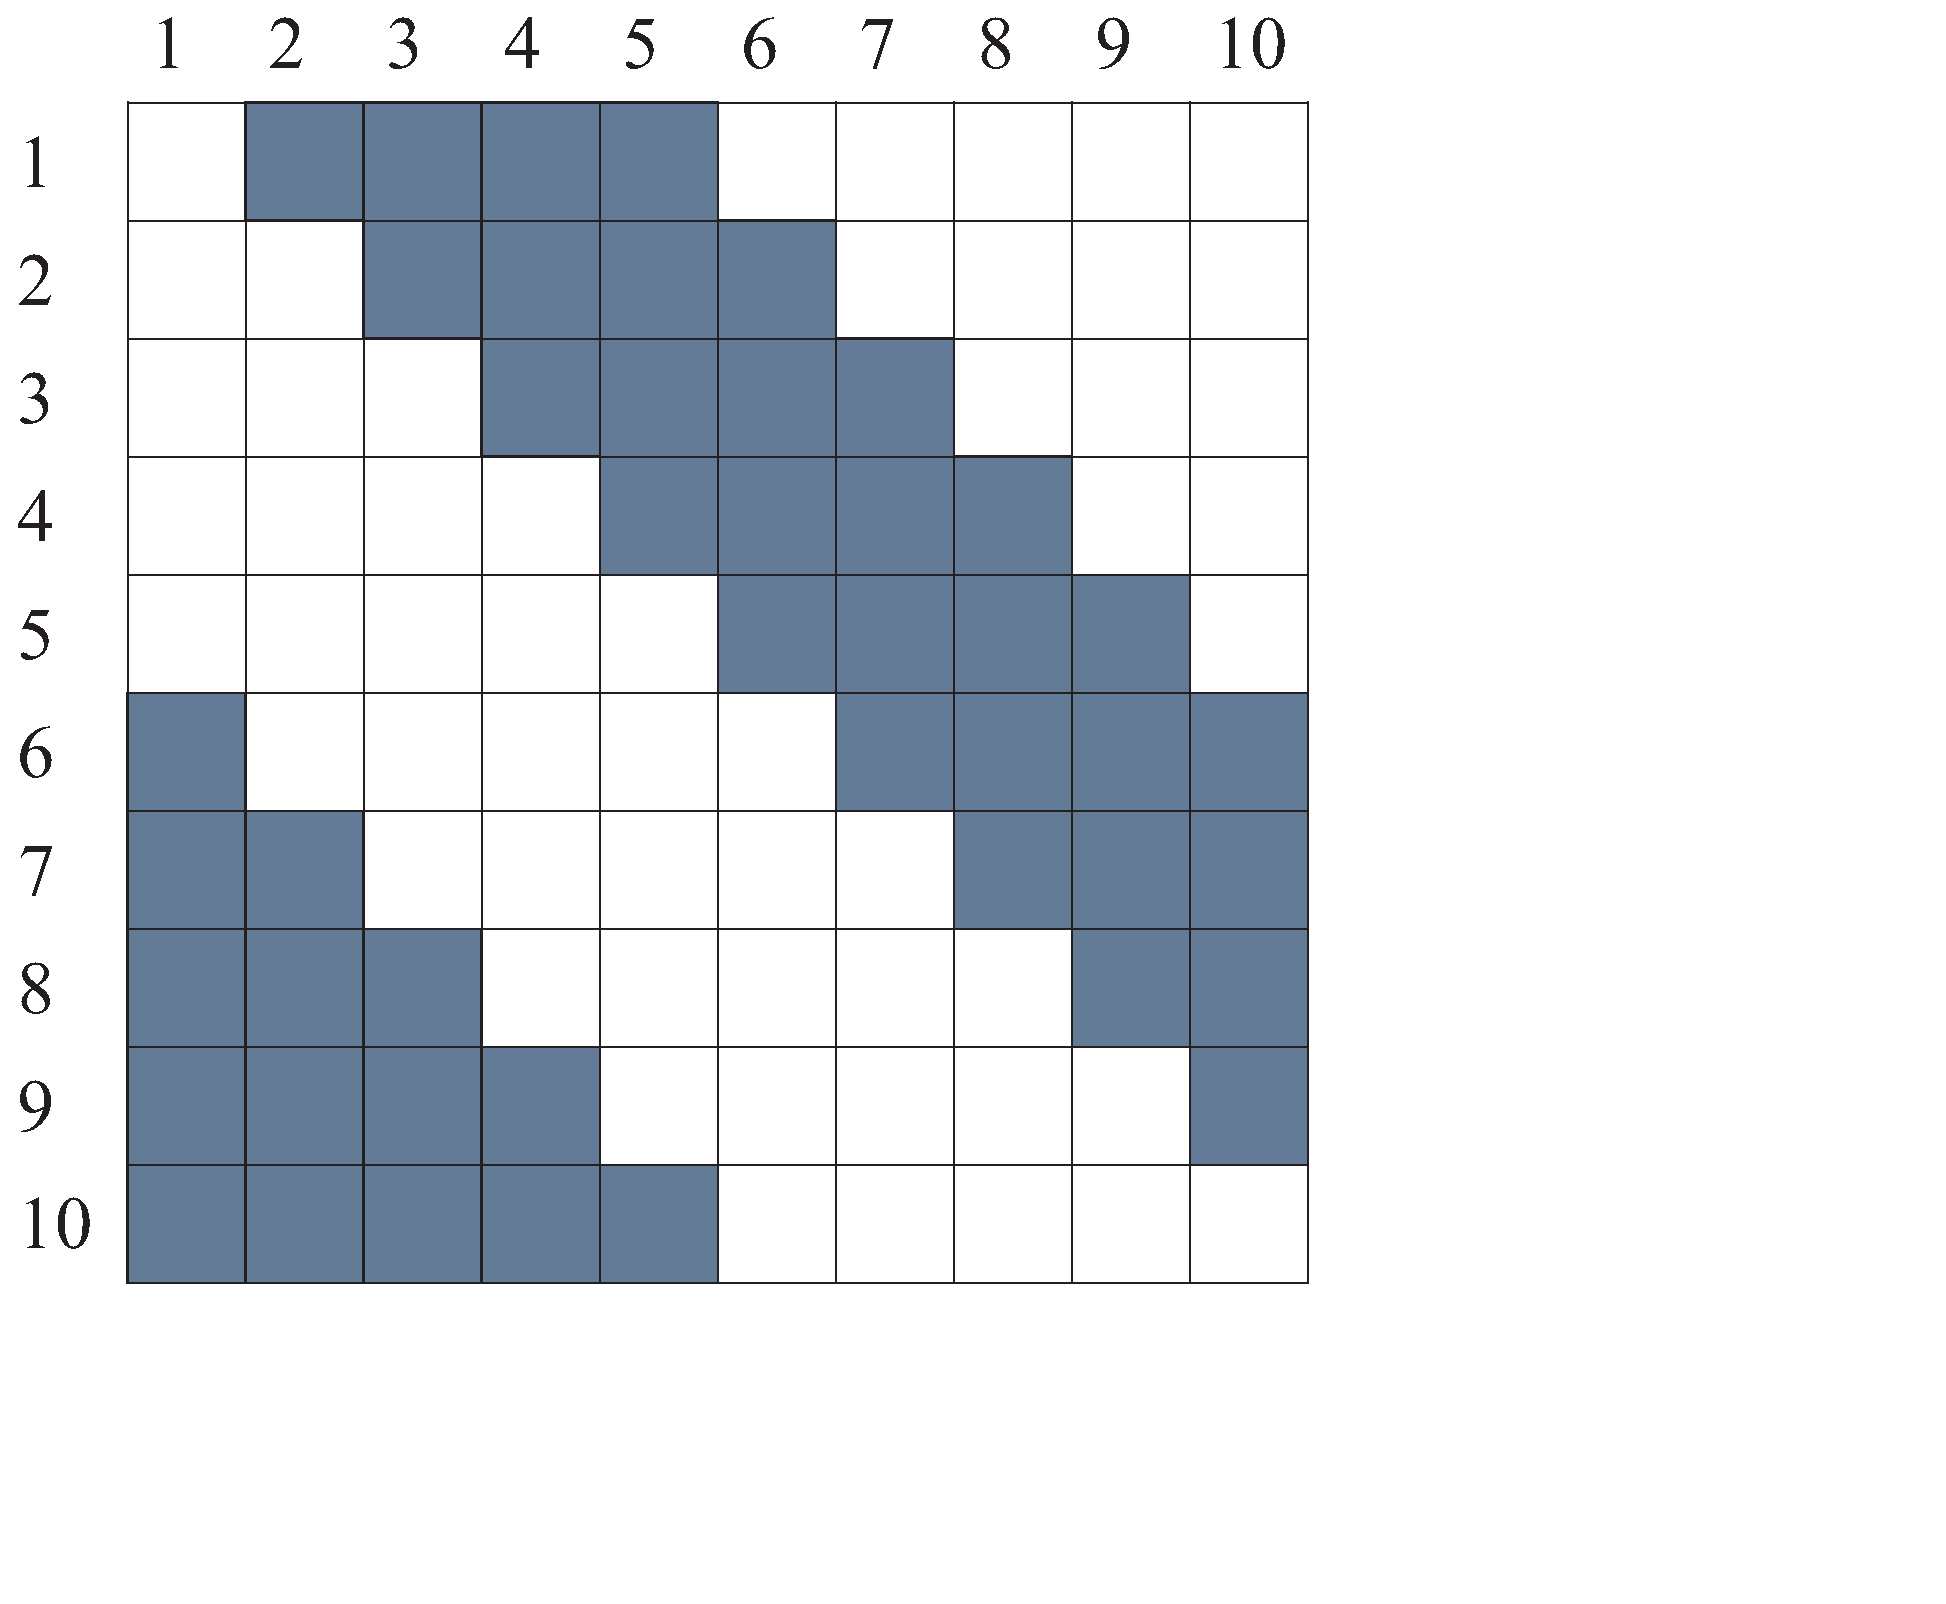
\includegraphics[width=7cm]{fig_Plimpton}
	\end{center}
	\caption{Schematic of the molecule decomposition parallelization by Plimpton~\cite{plimpton1993}.}
	\label{ms2pic_plimpton}
\end{figure}
\newline\noindent
% DE: Explanation of Triviral MC parallelization
The MC code is parallelized exploiting the stochastic nature of the simulation method. Starting from an equilibrated state in the simulation volume, the molecular configuration is copied multiple times into different volumes. Then, each copy runs  independently in parallel, but with a different random number seed, to calculate the thermodynamic properties. At the end, the data from all copies are gathered and averaged.



\section{Vectorization \& Memory}
\label{sec:Vectorization Memory}

The program $ms2$ specifically accounts for vector-parallel machines. All the main information needed in the computationally costly 
inner loops of the calculation, like the positions of the molecules and their sites, are stored in vectors that are accessed sequentially. 
This allows for an efficient use of memory on vector-parallel machines. \\ 
% 
For the evaluation of one configuration in $ms2$, e.g. the position vectors are loaded once and then distributed among all processors. 
Then, additional information like interaction partners of each individual molecule is computed, tabulated in vectors and communicated. 
The order of this data follows the order of all other vectors, e.g. the position vector. An example of a storage vector is shown 
in Table~\ref{vector_ex}.
The appropriate order allows for a serial access to the data in all vectors in the random access memory. 
Therefore, the calculations can be vectorized, increasing the efficiency. 
% 
\begin{table}[ht]
	\noindent
	\caption{Listing of the interaction partners for a molecule $i$, indicating the assembly in the storage vector.}
	\label{vector_ex}
	\begin{center}
		\begin{tabularx}{300pt}{c|X X X X X } 
			\hline
			\hline
			Molecule $i$ & \multicolumn{5}{c} {Interaction list for molecule $i$ within the storage vector}\\
			\hline
			1           &     2 & 4 & 6 & ... & 10 \\
			3           &       & 4 & 7 & ... & 10 \\
			4           &       &   & 8 & ... & 10 \\
			\hline
			\hline
		\end{tabularx}
	\end{center}
\end{table}


\section{Benchmarks/ Test case}
\label{sec:Benchmarks/ Test case}


% siehe erstes release paper Section 5


\section{Structure of program code}
\label{sec:Structure of program code}


This section discusses the code design and implementation issues of $ms2$ in detail. These explanations of the source code are 
intended to help understanding the program and to encourage the reader to further develop and improve the code.
\noindent 
New developers should get a smooth entry and the possibility to make fast adaptations to new problems.
Due to the experience of the core developers and the suitability for an efficient numerical code, Fortran90 was chosen as programming language. 
The program makes extensive use of the concepts introduced with Fortran90, notably modular programming.
% 
\noindent A wide variety of different simulation setups is possible, each requiring different 
computations. The most significant difference between the setups lies with the choice of MD or MC. While MD features extensive force 
calculations in order to update the molecular positions, MC is based on a Markov chain, where a molecular move is accepted with a certain 
probability. However, there are many other choices regarding the setup. This variety leads 
to a strong need for a highly modular structure, where modules have clear-cut interfaces. Given such a modularity, 
the appropriate functionalities can be combined to the desired simulation, while leaving out any unnecessary 
code\footnote{Unnecessary for the current setup.}. Besides avoiding if-statements at computationally demanding points and therefore 
leading to a better data flow, this allows for an efficient implementation of new functionalities, as existing modules can be used 
whenever feasible. In $ms2$, a stringent philosophy regarding modularization was followed, which is discussed in section~\ref{subsec_modstruc}.
% 
\noindent The runs need to be fast and scale well with increasing number of processors in order to achieve short response times. $ms2$ is parallelized with the Message Passing Interface~(MPI)~\cite{Forum2009}. While MD needs synchronization after 
every time step due to its deterministic nature, MC can be run embarrassingly parallel, only requiring synchronization at the very 
end of a run\footnote{Therefore, parallelization can be achieved by simply executing multiple MC runs simultaneously and averaging 
	over all runs, cf. section~\ref{subsec_parallel}.}. 
% 
\noindent Furthermore, the by far most expensive part of the code, calculating forces and potential energies, is highly vectorized 
and optimized.


-----

In order to keep the class hierarchy flat, $ms2$ does not make use of inheritance and hence polymorphism. 
E.g. the module \lstinline{ms2_site} contains the classes \lstinline{TSiteLJ126}, \lstinline{TSiteCharge}, \lstinline{TSiteDipole} 
and \lstinline{TSiteQuadrupole}, which have data and functionalities in common, but they are not derived from a common class.
\begin{figure}
	\begin{center}
		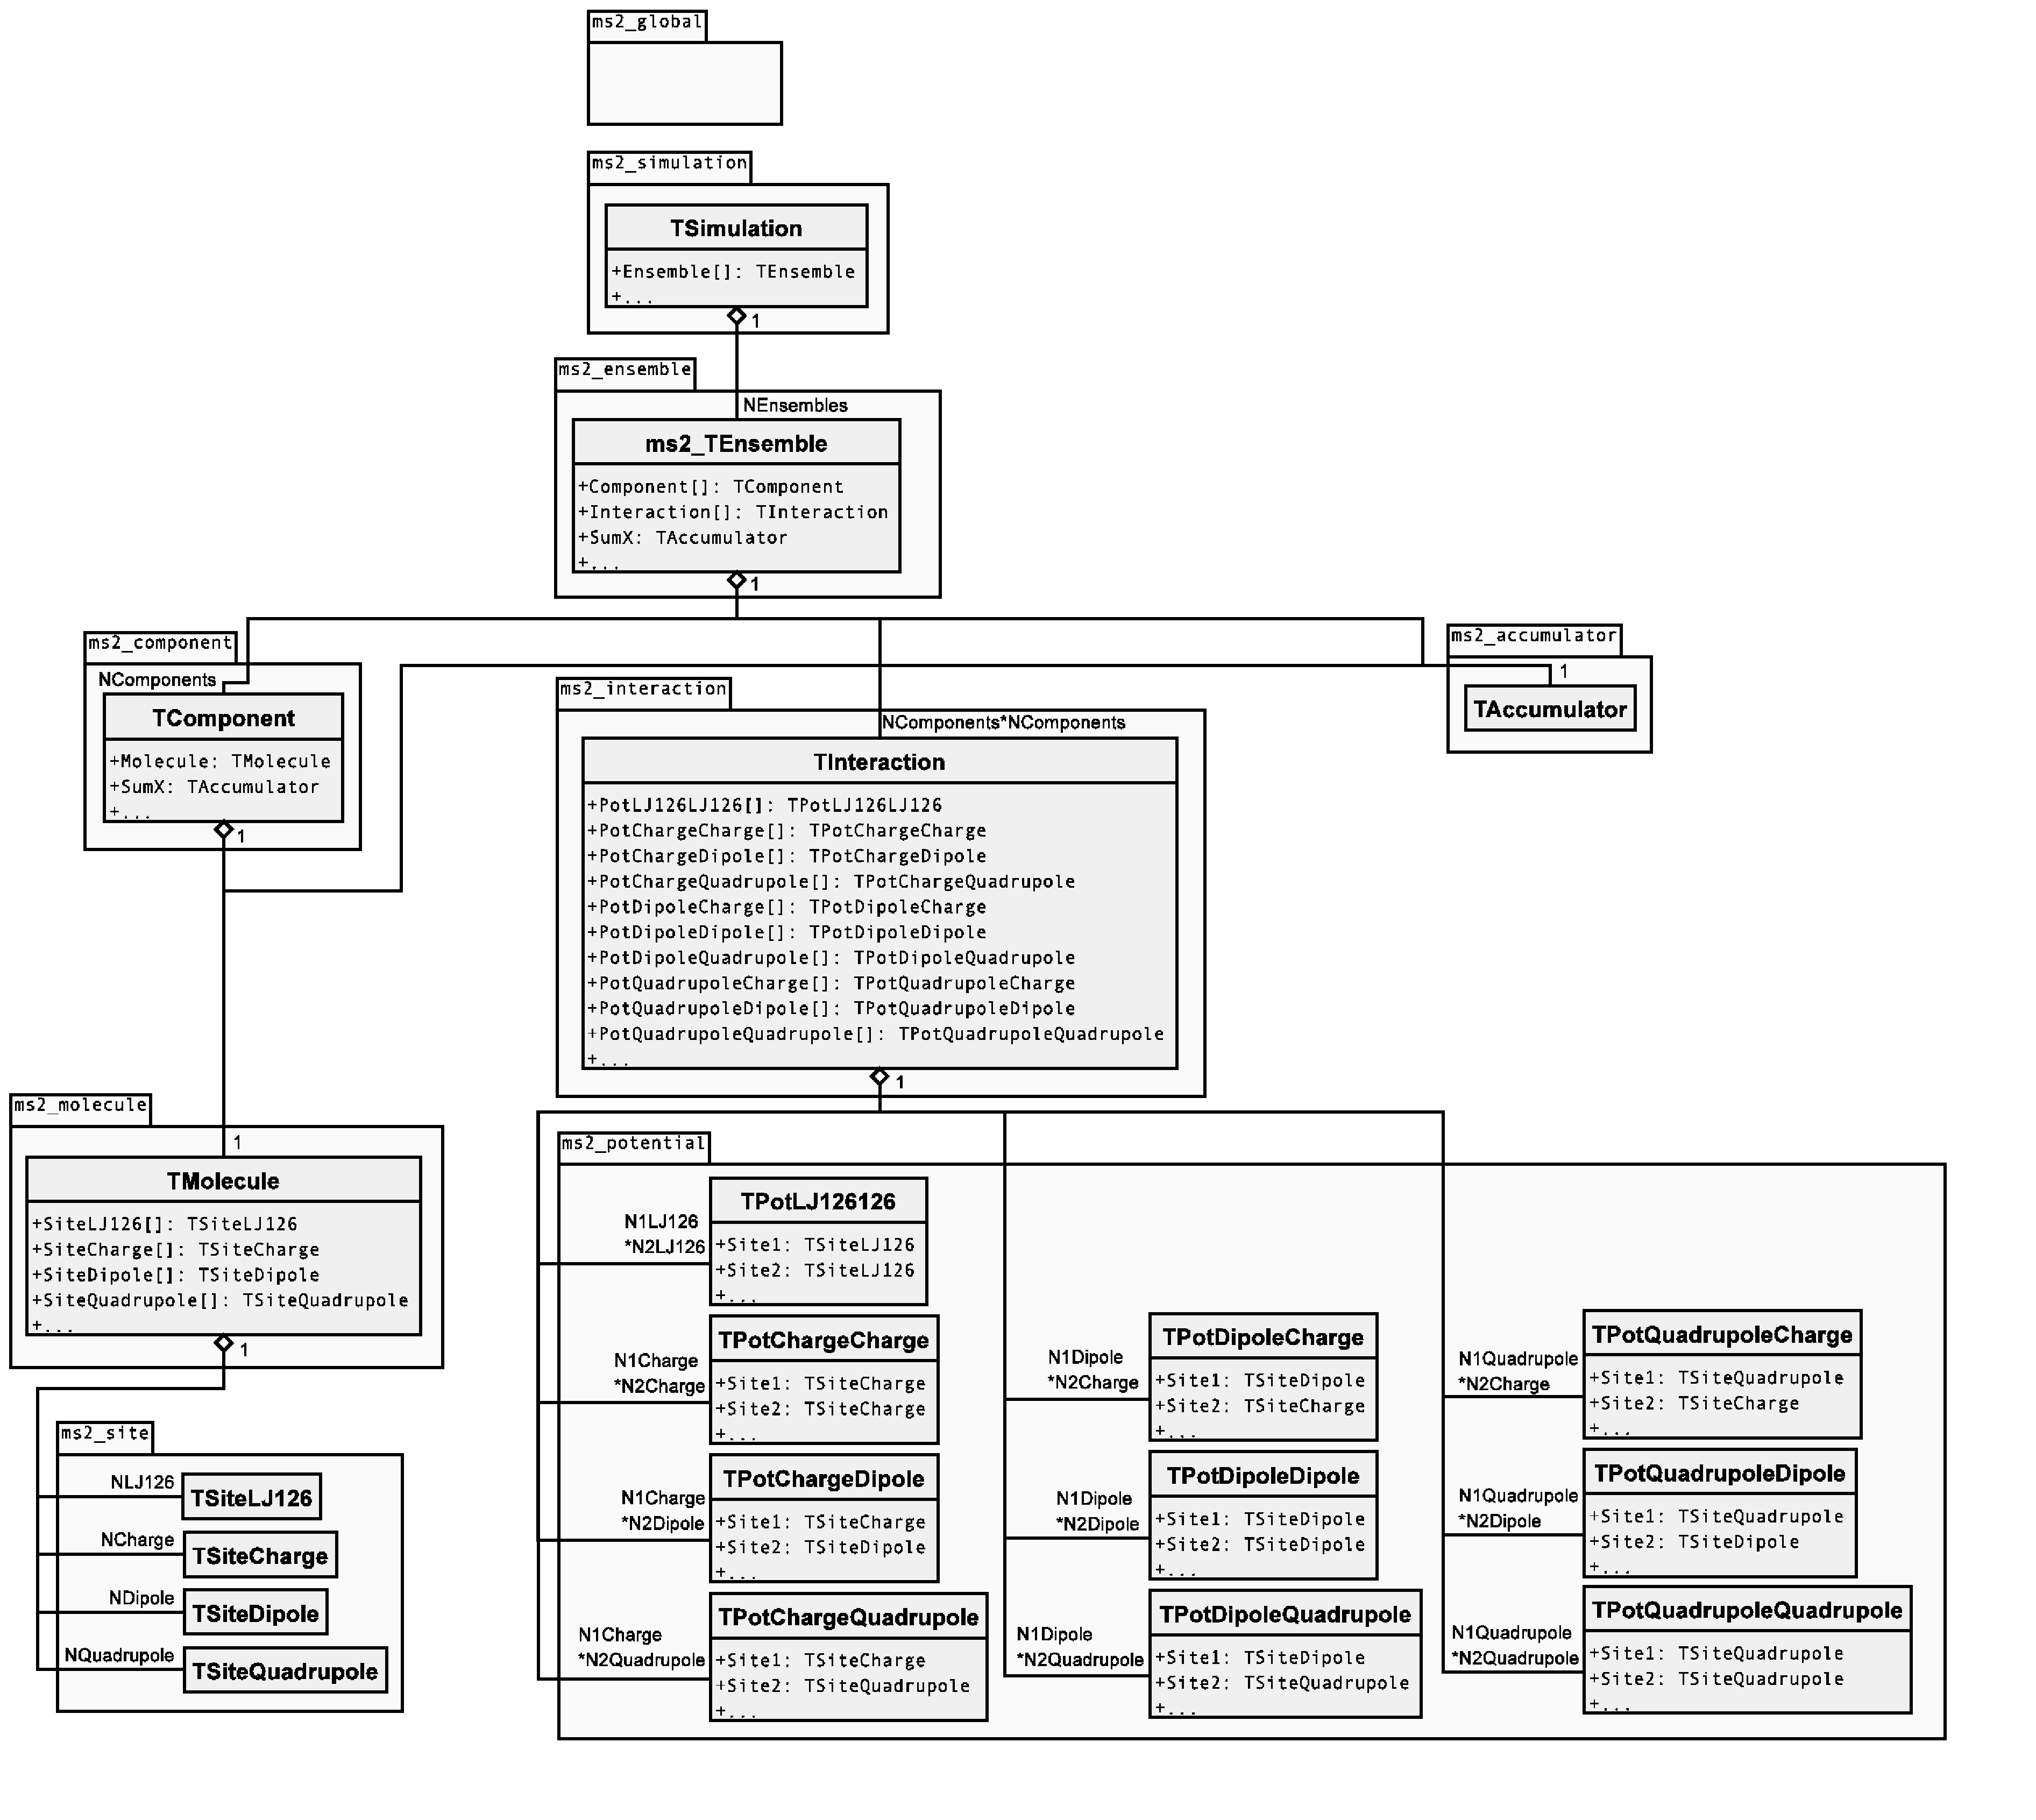
\includegraphics[width=\textwidth]{fig_ms2_modules_1.eps}
		\caption[aboveskip=0.5cm]{UML class diagram of $ms2$, showing object attributes.}
		\label{pic_ms2modules}
	\end{center}
\end{figure}
% 
\noindent The class structure and the relations between the classes is organized in six levels, as depicted in Figure~\ref{pic_ms2modules}.
% 
% 
% 
Every class is located on a certain level and hence has data and modules relevant to its level. 
The six levels are intuitive:
% 
\begin{enumerate}
	\item Global -- all data and functions of global use are handled. Scope: whole code
	\item Simulation -- setup and control of the simulation. Scope: simulation framework
	\item Ensemble -- the required ensemble is set up and initialized. Scope: molecular ensemble
	\item Component -- data and functions dealing with all molecules of a given molecule type. Scope: one molecule species
	\item Molecule -- data regarding the basic structure of a molecule. Scope: one molecule 
	\item Site -- position of sites with respect to a molecule. Scope: site of one molecule
\end{enumerate}


\textbf{First level - global}
The first level contains subroutines and variables that are needed globally in all parts of the simulation. The variables are mainly natural 
constants like the Boltzmann constant $k_{\mathrm B}$, the Avogadro constant $N_A$, etc. Additionally, variables defining the simulation 
setup for the given run are stored, e.g. the simulation technique and the ensemble type. 
These variables determine the type of calculation and are assigned according to user specifications on subsequent levels in $ms2$.
Subroutines that are stored on this level are also of global use in $ms2$. These are basic routines for input into the simulation tool and 
output into files, as well as more advanced routines for automated communication between hardware and program via signals. The latter routines 
are of particular interest for running $ms2$ on high performance clusters, where possible data loss can be avoided by automated communication 
between cluster nodes and the program.
% 
\textbf{Second level - simulation}
On the second level, the simulation flow is controlled. The simulation is initiated, started and sustained. This includes controlling the 
length of the simulation and its output, which is further discussed in section~\ref{sec_io}. User specifications concerning the simulation 
setup are read and the corresponding  global variables are assigned accordingly. Furthermore, all simulation quantities and averages are 
analyzed and written to file.
% 
\textbf{Third level - ensemble}
On the third level, the simulation is organized according to the desired ensemble specified by the user.
The respective ensemble is initialized, by characterizing the ensemble setup and defining e.g. the volume and the composition of the 
molecular species in the simulation volume. 
\noindent In addition, the initial positions and velocities of all molecules are distributed. Furthermore, the routines for the subsequent 
simulation are assigned on this level. The time evolution or the Markov chain, respectively, is performed and the ensemble averages 
of thermodynamic properties are calculated during the simulation run. 
% 
\textbf{Fourth level - component}
On this level, the molecule species (component) and their interactions are addressed. The class structure has three distinct 
branches. While the first branch deals with issues regarding structure and properties of one component at a time, 
the second branch deals with interactions between molecules of one or two components. 
The third branch contains all routines for the accumulation of data, determining the average value of the data as well as their statistical 
uncertainties. The first two branches will be discussed in more detail.\\
The first branch deals with the structure of one individual component. An instance of the class component stores center of mass 
position, orientation, velocity etc. of every molecule of one species, e.g. H$_2$O. The contained modules deal with calculations 
all molecules of this species, e.g. modules for solving Newton's equations of motion, kinetic energy calculation, atom to molecule 
transformation and vice versa. Furthermore, this branch is responsible for the correct initialization. 
It reads the molecular model for every component, calculates positions, introduces the reduced quantities, etc.\\
The second branch deals with interactions between molecules of one or two components. Therefore, this branch contains all force and 
potential energy calculations, which are the computationally most expensive parts by far. This branch is highly vectorized to achieve a fast 
calculation, in particular if executed in vector-parallel. The modules in this branch are simulation technique specific, i.e. MD or MC. 
\noindent
In a MD simulation, first, the interaction partners of every molecule are determined,  i.e. other molecules or sites within the 
cut-off radius. Then the interaction energies and virial contributions as well as the resulting forces and torques are calculated and 
summed up for every molecule. \\  
In a MC simulation, the modules are designed to calculate only the energy and the virial. Forces are not calculated and the 
corresponding algorithms are therefore entirely omitted in these modules.
\noindent
For MD, all interactions of one component-component pair\footnote{Please note that a component-component pair can consist of 
	one component paired with itself.} are calculated in one call of the module and they are therefore called once for every component-component 
pairing. For MC, the modules are finer-grained, calculating all interactions of one component-component pair by determining every 
molecule-molecule interaction individually. The corresponding modules are thus called more frequently than in case of MD.
% 
\textbf{Fifth level - molecule}
The basic information on molecules is stored on this level, such as mass, moment of inertia tensor, 
rotational degrees of freedom, etc. Higher level modules access this data via the class molecule.

\textbf{Sixth level - site}
Here, the assembly of a molecule is stored. The data is used by higher level modules to calculate the site positions 
from the molecular positions and orientations. This allows for the calculation of site-site interactions. It should be noted that $ms2$ only 
integrates (MD) or accepts (MC) center of mass positions and orientations. Site specific data is calculated for every simulation step on the fly.
% 

\textbf{Example}
The modular structure is discussed by highlighting the calculation process of a MD simulation of a pure fluid modeled by two LJ~sites 
and two point charges in the $NVT$ ensemble. 
During the initialization process, the modules for memory allocation and definition of the simulation scenario are executed. 
This process is not unique for one of the hierarchical levels, but takes places on all levels, cf. Figure~\ref{pic_ms2modules}. 
On level one, the simulation is delimited to "molecular dynamics", therefore all modules concerning MC simulation are neglected entirely. 
On level two, the "initialization" modules define the simulation environment by setting ensemble specific properties like simulation volume, 
temperature as well as the thermostat and integration scheme, etc. While the use of the first modules mentioned here is required 
in each simulation, independently of MD or MC, e.g. the trajectory calculation is specific for MD. However, the modular 
structure helps keeping the efficiency of the program by initiating only the simulation-specific molecule propagation.
The same effect of modules can be found in the initiation process on lower levels. Here, the exact composition of the molecular species 
in the simulation volume (module component), the description of the molecule (module molecule) and the storage of the positions, 
velocities and forces of all LJ~sites and charges (module sites) is determined. 
All other modules, like treating additional components for mixtures or containing characteristic properties of dipoles or 
quadrupoles, are fully omitted by $ms2$, since these are not used throughout this simulation.
% 
% 
Once the simulation has been initialized, a set of modules is invoked, which deals with maintaining the molecular simulation. 
On level one, this includes modules of global use for any simulation, e.g.~limiting the execution time, etc. 
On level two, Newton's equations of motion are numerically integrated, requiring information about the fluid's composition, 
the positions and orientations of the molecules etc. provided by modules of the respective level. The thermostat is applied and the 
calculation of thermodynamic properties is performed. The forces, torques and energies are calculated  in the second branch 
on the level component. For a MD simulation, this covers routines for the calculation of energies as well as forces at the same time, 
whereas in contrast for a MC simulation, the modules only calculate energies and virial contributions. 
% 
A further set of modules deals with the accumulation of data. These modules are designed to store data and evaluate the statistics of 
the produced data. The actual thermodynamic properties are calculated on the ensemble level. 
% 
The last set of modules deals with the output, where the results of the molecular simulation are written to file. These modules are called 
independent on the user settings in all simulation scenarios. 




\chapter{Tools}
\label{sec:Tools}

The tools described in the following are intended to facilitate the handling of \textit{ms}2. They should allow for an easy start of molecular simulations with \textit{ms}2 and give access to all output data generated by \textit{ms}2.


\section{\textit{ms}2par}
\label{sec:ms2par}


The GUI-based feature tool $ms2par$ allows for a convenient generation of *.par files according to user specifications, cf. Figure~\ref{pic_ms2par}. It assigns the molecular model, ensemble, thermodynamic state point, time step, number of equilibration steps, etc. Furthermore, the tool proposes a cut-off radius based on the input data. After the user completes the specifications, the program generates the file *.par in ASCII format, to be read by $ms2$. Applying $ms2par$ is simple and should be intuitive even for new users. $ms2par$ is a java application, thus it runs independently on all operating systems. 


\section{\textit{ms}2potmod}
\label{sec:ms2potmod}



\section{\textit{ms}2chart}
\label{sec:ms2chart}


$ms2chart$ is a GUI-based java applet for evaluating the simulation results from $ms2$, cf. Figure~\ref{pic_ms2chart}. This tool plots the evolution of properties calculated by $ms2$. The properties shown on the different graph axes are chosen from a drop 
down menu and the plot is shown directly in the GUI. \\
For a better analysis, $ms2chart$ allows various features: plotting block averages as well as simulation averages into the same plot, changing the design of the plot, individual labeling of the axes and adjusting the frame detail of the plot. All plots can be exported in png~format. If needed, the simulation details can be displayed, i.e. the specifications in the *.par file, the results in the~*.res file and the summary in the~*.log file. \\
The analysis program $ms2chart$ can be executed at any time of the simulation, i.e. also while the simulation is still ongoing. There is no loss of data, if it is run on the fly. The tool $ms2chart$ is easy to understand and can be handled intuitively. It allows for an easy first analysis of the $ms2$ simulation results. Advanced users will use $ms2chart$ for a quick check of their simulation results, such as whether the equilibration time was appropriate or for a fast analysis, which is important if extensive series of simulation runs are performed.

\pagebreak

\section{\textit{ms}2molecules}
\label{sec:ms2molecules}
 

The program $ms2molecules$ is a visualization tool for $ms2$. The program displays the molecular trajectories that are stored 
by $ms2$ as a series of configurations in the *.vim file. $ms2molecules$ visualizes molecular sites by colored spheres. The colors are user defined. The size of a sphere is by default proportional to the LJ~size parameter $\sigma$, but can be changed manually in the first lines of the *.vim-file. This feature facilitates monitoring a component of interest by reducing the size of other components, e.g. solvents. Other features like zooming in or out of the simulation volume and rotating the simulation box also facilitates the analysis of the simulation. The visualization can be exported via snapshots in the jpg~format. \\
The program is based on OpenGL and written in C. The handling of the program is simple and console based. Requirements for the feature tool are OpenGL in a Windows or Linux environment. Figure~\ref{pic_ms2molecules} shows a snapshot of a ternary mixture, taken with the program $ms2molecules$, which is convenient to gain insight into the trajectory of the system, or the state of the system, respectively.\\

\textbf{Colors:}\\
Setting the colours of the molecules in the visualisation window has to be done manually in the header of the \texttt{*.vim}-file (see section \ref{sec:vim - file}). The particle colour is defined by the last integer value of each line in the header, which makes the visualisation easy ajustable. The colour of each cite-type of each molecule-type in the simulation can be set separately. The available colours are:
\begin{table}[htbp]
	\centering
	\caption{Available Colours in \textit{molecules}}
	\begin{tabular}{rl}
		\toprule
		Integer in vim file & Colour \\
		\midrule
		1     & black \\
		2     & red \\
		3     & orange \\
		4     & yellow \\
		5     & yellow 2 \\
		6     & green \\
		7     & green 2 \\
		8     & turquoise \\
		9     & blue \\
		10    & blue 2 \\
		11    & purple \\
		12    & pink \\
		13    & pink 2 \\
		14    & grey \\
		\bottomrule
	\end{tabular}%
	\label{tab:Colours in vim file}%
\end{table}%




\textbf{Adjusting Atom size:}\\
The atom size, or the size of one cite in a molecule-type can be adjusted manually by the user in the header of the \texttt{*vim}-file. That can be done by setting the sigma-values of each cite, e.\,g.
\begin{Verbatim}
~  1 LJ  0.0000 -0.3387 -1.4713  3.0  1
~  1 LJ -0.0000  0.8836  0.0917  1.42  2
~  1 LJ -0.0000 -0.4503  1.1711  1.8  3 
\end{Verbatim}
The integer "1" in the first column after the tilde, specifies the LJ-cites as one of the 1st molecule (used \texttt{*pm} file). The 2nd, 3rd and 4th numeric column are the coordinates of the cite relative to the centre of mass of the molecule. The 5th column indicates the sigma value of the cite and can manually re-adjusted. The last integer column indicates the colour of the cite (see above). 

\pagebreak

\section{res2gepar}
\label{sec:res2gepar}
% Minh









%\begin{Verbatim}[frame=single,framesep=6.5mm,label=\fbox{Example file 1 },numbers=left,numbersep=-10pt,xrightmargin=5cm]
%\end{Verbatim}

\chapter{Examples \& Tutorials}
\label{sec:Examples Tutorials}
% Andreas / Simon

% Input und Output kurz erläutern.

This part of the manual deals with example applications, where the use of the provided software will be demonstrated. The examples presented in this section were chosen such that a wide class of applications is covered. Each problem is briefly described and the appropriate input files are given. also includes some output files. 


\section{Lennard-Jones fluid}
\label{sec:Lennard-Jones Fluid}

An example for a complete *.par file is given below for a MD simulation of the Lennard-Jones fluid in the \textit{NVT} ensemble, where the chemical potential is calculated by the Widoms's test molecule method. In addition, the calculation of the transport properties is enabled.



Parameters and options specified in the *.pm file for the Lennard-Jones fluid:\\\\

\begin{Verbatim}[frame=single,framesep=6.5mm,label=\fbox{Lennard-Jones fluid},numbers=left,numbersep=-10pt,xrightmargin=5cm]
# MS2 Parameterfile created with ms2par
# General simulation parameters
Units         =       Reduced
LengthUnit    =       1.0
EnergyUnit    =       1.0
MassUnit      =       1.0 
Simulation    =       MD
Integrator    =       Gear
TimeStep      =       0.0010
Ensemble      =       NVT
MCORSteps     =       0
NVTSteps      =  300000
RunSteps      = 1000000
ResultFreq    =    1000
ErrorsFreq    =    5000
VisualFreq    =       0
CutoffMode    =       COM
NEnsembles    =       1
CorrfunMode   =       yes
#
# Ensemble 1
#
Temperature   =       1.10
Density       =       0.66
OptPressure   =       Yes
NParticles    =    1372
NComponents   =       1
Corrlength    =    6000
SpanCorrfun   =     300
ViewCorrfun   =     100
ResultFreqCF  =       1

PotModel      =       lj.pm
MoleFract     =       1.0
ChemPotMethod =       Widom
NTest         =    3000

Cutoff        =       6.3
Epsilon       =       1.0E10
\end{Verbatim}

\vspace{1cm}






\section{Vapour-Liquid Equilibrium of a \ce{O2} -- Aceton mixture}
\label{sec:Vapour-Liquid Equilibrium of a O2 - Aceton mixture}

\begin{Verbatim}[frame=single,framesep=6.5mm,label=\fbox{VLE \ce{O2} -- Aceton mixture},numbers=left,numbersep=-10pt,xrightmargin=5cm]
#
# MS2 Parameterfile created with ms2par
#

#
# General simulation parameters
#
Units       =       SI
LengthUnit  =       3.5
EnergyUnit  =       100.0
MassUnit    =       40.0
Simulation    =      MC
Acceptance    =      0.5
Ensemble      =      GE
NVTSteps      =   10000
mueVTSteps    =   25000
RunSteps      =  200000
ResultFreq    =     100
ErrorsFreq    =    1000
VisualFreq    =       0
CutoffMode  =       COM
NEnsembles    =       1

#results from liquid run
Temperature = 400.00   
Pressure0     =       9.000
LiqDensity    =      11.5790
VarDensity    =       0.0051
LiqEnthalpy   =  -23452.3
VarEnthalpy   =       8.4
LiqBetaT      =       0.004760
VarBetaT      =       0.000252
LiqdHdP       =      -0.001457
VardHdP       =       0.004658

#parameters for vapor run
Density       =       1.000
OptPressure   =     Yes
NParticles    =     500
NComponents   =       2

PotModel      =      O2.pm
MolarFract    =       0.5000
LiqMolarFract =       0.0799
ChemPot       =      -2.849
VarChemPot    =       0.003
PartMolVol    =       3.4185
VarPartMolVol =       0.1899


PotModel      =  aceton.pm
MolarFract    =       0.5000
LiqMolarFract =       0.9201
ChemPot       =      -5.246
VarChemPot    =       0.011
PartMolVol    =       3.5289
VarPartMolVol =       0.3598

eta         = 1.0
xi          = 0.905
Cutoff      = 4.0
Epsilon     = 1.0E10
\end{Verbatim}



\section{calculating configurational properties}
\label{sec:calculating configurational properties}





\section{calculating transport properties}
\label{sec:calculating transport properties}






\section{chemical potential by ThermoInt}
\label{sec:chemical potential by ThermoInt}




\section{\ce{NaCl}-Water Solution \& osmotic pressure}
\label{sec:NaCl-Water Solution osmotic pressure}





\section{multi-Ensemble method}
\label{sec:multi-Ensemble method}




\section{humid air ensemble}
\label{sec:humid air ensemble}


















\chapter{Error Messages}
\label{sec:Error Messages}
% 

\input{Literature.tex}




%************************************************************************
% Nachspann
%
%************************************************************************

% Einfügen des Literaturverzeichnis
\printbibliography

\appendix

% Einfügen der Anhänge
%\input{anhang.tex}


% keine Nummerierung der nachfolgenden Kapitel
\backmatter

% Einfügen des Symbolverzeichnis
{ % Tabellendefinitionen gelten nur in diesem Dokument

% Longtable auf Spaltebreite ausdehnen
\setlength\LTleft{0pt}
\setlength\LTright{0pt}
% Definition neuer Spaltentypen
\newcolumntype{Z}{>{$}p{0.15\linewidth}<{$}} % Symbol (mit Matheumgebung)
\newcolumntype{A}{>{\bfseries} p{0.15\linewidth}} % Abkürzung (fett)
\newcolumntype{B}{l @{\extracolsep{\fill}}} % Beschreibung


\chapter{Symbolverzeichnis}

\section*{Formelzeichen}

\begin{longtable}{Z B r}
\textbf{Symbol} & \textbf{Bedeutung}         & \textbf{Einheit} \\
\addlinespace
\endhead
% Symbolspalte wird immer in Matheumgebung gesetzt --> $ $ nicht nötig
%************************************************************************
a               & Länge                      & \SI{}{m}         \\
b               & Breite                     & \SI{}{m}         \\
c               & spezifische Wärmekapazität & \SI{}{kJ/(kg.K)} \\
\ell            & charakteritische Länge     & \SI{}{m}         \\
Re              & Reynoldszahl               &                  \\ 
w               & Strömungsgeschwindigkeit   & \SI{}{m/s}       \\ 
%************************************************************************
\end{longtable}


\section*{Griechische Symbole}

\begin{longtable}{Z B r}
\textbf{Symbol} & \textbf{Bedeutung}         & \textbf{Einheit} \\
\addlinespace
\endhead
% Symbolspalte wird immer in Matheumgebung gesetzt --> $ $ nicht nötig
%************************************************************************
\lambda         & Wärmeleitfähigkeit         & \SI{}{W/(m~K)}   \\ 
\nu             & kinematische viskosität    & \SI{}{m^2/s}     \\
\varrho         & Dichte                     & \SI{}{kg/m^3}     \\
%************************************************************************
\end{longtable}


\section*{Indizes}

\begin{longtable}{Z l} 
\textbf{Symbol} & \textbf{Bedeutung} \\
\addlinespace
\endhead
% Symbolspalte wird immer in Matheumgebung gesetzt --> $ $ nicht nötig
%************************************************************************
\mathrm{L}      & Luft               \\
\mathrm{p}      & isobar             \\
%************************************************************************
\end{longtable}



\chapter{Abkürzungsverzeichnis}

\begin{longtable}{@{} A l @{}}
%************************************************************************
eps & Encapsulated PostScript  \\
pdf & Portable Document Format \\
svg & Scalable Vector Format   \\
%************************************************************************
\end{longtable}
}


\setcounter{table}{0}
% setzt den Tabellenzähler zurück, damit das Symbolverzeichnis
% nicht mitgezählt wird


%%% Local Variables: 
%%% mode: latex
%%% TeX-master: "master"
%%% coding: utf-8
%%% End: 

% erzeugt den Index aus den Einträgen \index{Eintrag}
\renewcommand{\indexname}{Stichwortverzeichnis}
\printindex

\end{document}


%%% Local Variables:
%%% coding: utf-8
%%% End:

